\documentclass[12pt,a4paper]{article}

% Sprache, Input, etc.
\usepackage[utf8]{inputenc}
\usepackage[T1]{fontenc}
\usepackage{lmodern}
\usepackage{hyphsubst}
\usepackage[english,ngerman]{babel}
%\usepackage{eurosym}

% Mathepakete
\usepackage{amsmath,amsthm,amssymb,mathtools,amsfonts}

%Darstellung von mathematischen Symbolen
\usepackage{yfonts,dsfont}
\usepackage{textcomp}

% für Normalverteilungs-Ns
\usepackage{mathrsfs}

%\usepackage{blindtext}

% A4 Papier benutzen
\usepackage{a4wide}

% für Programmcode
% \usepackage{listings}

% für die Bibliographie
\usepackage[backend=biber, style=ieee-alphabetic]{biblatex}
\usepackage[babel,german=guillemets]{csquotes}
\addbibresource{literature.bib} 

% Abbildungen
%\usepackage{graphics}
\usepackage{graphicx}
\graphicspath{{graphics/Beispiel/}{graphics/Stammzellen-10kPa/}{graphics/Stammzellen-30kPa/}{graphics/Stammzellen-Vergleich/}}

%folgende Pakete werden nur zur schöneren Ausgabe des LaTeX-Quellcodes unten geladen.
\usepackage{listings}
\lstset{language=[LaTeX]TeX}
\HyphSubstIfExists{ngerman-x-latest}{%
  \HyphSubstLet{ngerman}{ngerman-x-latest}}{}
\HyphSubstIfExists{german-x-latest}{%
  \HyphSubstLet{german}{german-x-latest}}{}
\setlength{\parindent}{0em} 

%Zeilenabstände
\usepackage{setspace}
\usepackage{float}

%Tabellen
%\usepackage{tabularx}

%%%%%%%%%%%%%%%%%%%%%%%%%%%%%%%%%%%%%%%%%%%%%%%%%%%%%%%%%%%%%%%%%

% neue Umgebungen
\theoremstyle{definition}
\newtheorem{Definition}{Definition}[subsection]

\newtheorem{Beispiel}[Definition]{Beispiel}

\theoremstyle{definition}
\newtheorem{Satz}[Definition]{Satz}

\theoremstyle{definition}
\newtheorem{Simulation}[Definition]{Simulation}

\theoremstyle{definition}
\newtheorem{Lemma}[Definition]{Lemma}



%%%%%%%%%%%%%%%%%%%%%%%%%%%%%%%%%%%%%%%%%%%%%%%%%%%%%%%%%%%%%%%%%%%%%%%%%%%%%%%%%%%%%%%%%%%%%%%%%%%%%%
% Abkürzungen für das Beispiel
% für das Modell
\newcommand{\seedexample}{100}
\newcommand{\nobs}{50}
\newcommand{\betatrue}{(10,5,-4,7)}
\newcommand{\phitrue}{0.001}
\newcommand{\sigmatrue}{1}
\newcommand{\gradtrue}{3}
\newcommand{\maxy}{18.61206}

%%%
% Kapitel 1 Regression und KB
% Regression Grad Drei
\newcommand{\gradone}{3}
\newcommand{\betaoneest}{(0.54357174 ; 0.21282372 ; -0.03915277 ; 0.24840114)}
\newcommand{\sigmaoneest}{0.04455856}
\newcommand{\maxY}{ 18.62582 }
\newcommand{\betaesttrafo}{ (10.1169882 ; 3.9610873 ; -0.7287135 ; 4.6232562) }
\newcommand{\sigmaesttrafo}{0.8293265}

% für die Konfidenzbänder
\newcommand{\alphaKB}{0.05}
\newcommand{\cR}{3.20876}
\newcommand{\niter}{5000}
\newcommand{\cA}{3.143099}
\newcommand{\cAP}{2.79563}
% Feinheit des Grids, dass in minmaxpoly erzeugt wird, um die
% Nullstellen zu bestimmen
\newcommand{\ngridpoly}{100}

%%%
% Kapitel 2 Vergleich
% für die Regression mit Grad drei
\newcommand{\gradtwo}{4}
\newcommand{\betatwoest}{(0.5297226 ; 0.5882577 ; -1.7965271 ; 3.0540371 ; -1.4350387)}
\newcommand{\sigmatwoest}{0.04499058}

% Parameter für den vergleich
\newcommand{\TestWert}{655277.9}% Wert der Teststatistik
\newcommand{\kritWert}{2.422085}%Quntil beim Test
\newcommand{\EntscheidungHypothesen}{verwirft man}
\newcommand{\Modellesind}{verschieden}

\newcommand{\cVergl}{2.87904}

%%%
% Kapitel 4 abhängige Daten
% für die Regression mit Grad Drei mit AR
\newcommand{\betaARone}{ (0.54357174 ; 0.21282372 ; -0.03915277 ; 0.24840114) }
\newcommand{\sigmaARone}{0.04455856}
\newcommand{\phiestone}{-0.2918199}
\newcommand{\betaAResttrafo}{ (10.1169882 ; 3.9610873 ; -0.7287135 ; 4.6232562) }
\newcommand{\sigmaAResttrafo}{0.8293265}
\newcommand{\cAPAR}{2.817034}

\newcommand{\betaARtwo}{(0.5282983 ; 0.5347608 ; -1.5079080 ; 2.5435075 ; -1.1485678)}
\newcommand{\sigmaARtwo}{0.04416834}
\newcommand{\phiesttwo}{-0.2745721 }

\newcommand{\cVerglAR}{ 2.920874 }


% Matrixmultiplikationen im Beispiel darstellen
%\newcommand{\Ydat}{...}
%\newcommand{\Ydattext}{...}
%\newcommand{\Ytrafo}{...}

%\newcommand{\edat}{...}

%\newcommand{\Xidat}{...}
%\newcommand{\Xitrafo}{...}

%\newcommand{\Xtrafo}{...}
%\newcommand{\Xtwodat}[0]{...}
%\newcommand{\Xonedat}[0]{...}

\newcommand{\betatwodat}[0]{\left[ \begin{array}{c} \beta_{0,2} \\ \beta_{1,2} \\ \beta_{1,3} \\ \beta_{1,4} \end{array} \right]}
\newcommand{\betaone}[0]{\left[ \begin{array}{c} \beta_{0} \\ \beta_{1} \\ \beta_{2} \\ \beta_{3} \end{array} \right]}
\newcommand{\betaonedat}[0]{\left[ \begin{array}{c} \beta_{0,1} \\ \beta_{1,1} \end{array} \right]}

% Ungenutzt
%\newcommand{\betatrafoest}{...}
%\newcommand{\sigmatrafoest}{...}

%%%%%%%%%%%%%%%%%%%%%%%%%%%%%%%%%%%%%%%%%%%%%%%%%%%%%%%%%%%%%%%%%
% Parameter für die Simulation
% für das Modell
\newcommand{\ntest}{100}
\newcommand{\simgrad}{5}

% Die normalen
% ueberdeckung, R als Grundmodell
\newcommand{\UeberRR}{0.953}
\newcommand{\UeberRMinmax}{.956}
\newcommand{\UeberRMinmaxPoly}{0.83}
\newcommand{\UeberRMinmaxPolyfast}{0.951}

% ueberdeckung, AR bekannt als Grundmodell
\newcommand{\UeberARbekanntR}{0.94}
\newcommand{\UeberARbekanntMinmax}{0.93}
\newcommand{\UeberARbekanntMinmaxPoly}{0.67}
\newcommand{\UeberARbekanntMinmaxPolyfast}{0.90}

% ueberdeckung, AR als Grundmodell
\newcommand{\UeberARR}{1.00}
\newcommand{\UeberARMinmax}{1.00}
\newcommand{\UeberARMinmaxPoly}{0.03}
\newcommand{\UeberARMinmaxPolyfast}{1.00}

% Die Prüfdingen
% ueberdeckung, R als Grundmodelll pruefen
\newcommand{\UeberRRpruefen}{0.99}
\newcommand{\UeberRMinmaxPolyfastpruefen}{0.97}

% ueberdeckung, AR bekannt als Grundmodell prufen
\newcommand{\UeberARbekanntRpruefen}{1.00}
\newcommand{\UeberARbekanntMinmaxPolyfastpruefen}{1.00}

% ueberdeckung, AR als Grundmodell pruefen
\newcommand{\UeberARRpruefen}{1.00}
\newcommand{\UeberARMinmaxPolyfastpruefen}{1.00}

%%%%%%%%%%%%%%%%%%%%%%%%%%%%%%%%%%%%%%%%%%%%%%%%%%%%%%%%%%%%%%%%%%%%%%%%%%%%%%%%%%%%%%%%%%%%%%%%%%%%%%
% glossary
\usepackage[nonumberlist]{glossaries}
 
\makeglossaries

\loadglsentries{myglossaries}
 

%%%%%%%%%%%%%%%%%%%%%%%%%%%%%%%%%%%%%%%%%%%%%%%%%%%%%%%%%%%%%%%%%%%%%%%%%%%%%%%%%%%%%%%%%%%%%%%%%%%%%%
\begin{document}
\begin{titlepage}

\begin{center}


% Oberer Teil der Titelseite:
%\includegraphics[width=0.6\textwidth]{logo.pdf}\\[1cm]    

\textsc{\LARGE Georg-August-Universität Göttingen}\\
\textsc{Fakultät für Mathematik und Informatik}\\
\textsc{Institut für Mathematische Stochastik}\\[1.5cm]


\textsc{\Large Bachelorarbeit}\\[0.5cm]


% Title
\newcommand{\HRule}{\rule{\linewidth}{0.5mm}}
\HRule \\[0.4cm]
\begin{onehalfspace}
{ \LARGE \bfseries  Vergleich von Regressionsmodellen mittels gleichmäßiger Konfidenzbänder  }\\[0.4cm]
\end{onehalfspace}
{ \large \bfseries Comparison of regression models using simultaneous confidence bands}\\[0.4cm]

\HRule \\[1cm]


% Author and supervisor
\begin{minipage}{0.4\textwidth}
\begin{flushleft} \large
\emph{Autor:}\\
Rolf Tobias Hajo Henrik Henning Hause\\
\end{flushleft}
\end{minipage}
\hfill
\begin{minipage}{0.4\textwidth}
\begin{flushright} \large
\emph{Erstgutachter:} \\
Prof. Dr. Tatyana Krivobokova\\
\end{flushright}
\end{minipage}
\vspace{0.3cm}

\begin{minipage}{0.4\textwidth}
\begin{flushleft} \large
\emph{Abgabetermin:}\\
11.07.2017\\

\end{flushleft}
\end{minipage}
\hfill
\begin{minipage}{0.4\textwidth}
\begin{flushright} \large
\emph{Zweitgutachter:}\\
Jun.-Prof. Dr. Andrea Krajina\\
\end{flushright}
\end{minipage}
\begin{flushleft}
\begin{minipage}{0.4\textwidth}
\begin{flushleft} \large
\emph{Studiengang:}\\
B. Sc. Mathematik\\
\end{flushleft}
\end{minipage}
\end{flushleft}
\hfill

% Unterer Teil der Seite
%{\large \today}

\end{center}

\newpage 
\thispagestyle{empty}
\quad 
\newpage
\end{titlepage}
\newpage

\tableofcontents
\newpage
\thispagestyle{empty}
\quad 


\section*{Einleitung}
Diese Bachelorarbeit behandelt Methoden, um Regressionsmodelle zu vergleichen. Seien zwei Regressionsmodelle 

\begin{equation*}
Y_i = X_i \beta_i + e_i ,~ i \in \{1,2\}
\end{equation*}

gegeben. Dabei seien $Y_i=(Y_{i,1}, \ldots, Y_{i,n_i})'$ zwei Vektoren mit abhängigen Variablen.
 
Weiterhin seien $X_i$ zwei $n_i \times (p+1)$ Designmatrix mit festem Design. Das bedeutet, für $l \in \{ 1, \ldots, \min(n_1, n_2)\}$ ist die $l$-te Zeile von $X_1$ gleich der $l$-ten Zeile von $X_2$.

Weiterhin seien $\beta_i = (\beta_{i,0}, \ldots, \beta_{i,p})'$ zwei Koeffizientenvektor und  $e_i = (e_{i,1}, \ldots, e_{i,n_i})'$ zwei Vektoren mit Zufallsfehlern. Also sind $Y_1$ und $Y_2$ zwei Gruppen von Beobachtungen, die von den selben unabhängigen Variablen abhängen. 

Ein Beispiel, entnommen \cite[116]{Liu64}, ist zu vergleichen, wie das Alter den Blutdruck von Männern und Frauen beeinflusst. Man hat zwei verschiedene Beobachtungen $Y_1$ und $Y_2$, den Blutdruck der Männer und den Blutdruck der Frauen, und versucht diese Beobachtungen mit dem selben Modell $X_i$ zu erklären. Da man eventuell verschieden viele Beobachtungen hat, haben die $Y_i$ dann verschiedene Dimensionen.

Im Modell der gewöhnlichen linearen Regression ist $e_i \sim \mathscr{N}_{n_i}(0,\sigma^2 I_{n_i})$. Das Testproblem für den Vergleich von Regressionsmodellen ist

\begin{equation*}
H_{0} : \beta_{1} = \beta_{2}  \textbf{ vs. }  H_{1} : \beta_{1} \neq \beta_{2}
\end{equation*}

Dabei gleicht man die Dimensionen der $\beta_i$ an, indem man Nullen einfügt.

Dieser Test wird normalerweise mit einem F-Test durchgeführt. In dieser Ausarbeitung werden alternative, auf Konfidenzbändern basierende Methoden nach \cite{Liu64} betrachtet. Insbesondere die folgenden Spezialfälle sind von Interesse:

\begin{itemize}
\item Das Modell hat Polynomgestalt, das heißt die $l$-te ($1 \leq l \leq n_i $) Zeile der Designmatrix $X$ ist von der Form $(1, x_{i,l}, x_{i,l}^2, \ldots, x_{i,l}^p)$.
\item Den Fehlern liegt ein AR(1)-Prozess zugrunde, dass heißt $e_i \sim \mathscr{N}_{n_i}(0,\sigma^2 \Upsilon)$ mit $\Upsilon \neq I_{n_i}$.
\item Man vergleicht die Regressionsmodelle nicht direkt sondern prüft, ob ein Teil des Regressionsmodells nicht signifikant ist. Das heißt man unterteilt $\beta_1 = (\beta_{1,1}, \beta_{1,2})$ und prüft, ob $\beta_{1,2}$ signifikant gleich Null ist. 
\end{itemize} 

Die Motivation für diese Betrachtungen ist der Vergleich von verschiedenen Regressionsmodellen für Stammzellen.

Das Kapitel \ref{Regression und Konfidenzbaender} stellt die Konzepte der Regression und der Konfidenzbänder vor. Außerdem werden Methoden angegeben, wie für diese Regressionsgraphen Konfidenzbänder konkret zu berechnen sind. 

Das Kapitel \ref{Vergleich von zwei Regressionsmodellen} führt aus, wie man Regressionsmodelle mittels des F-Tests vergleicht. Danach werden, mit Hilfe der Methoden aus dem ersten Kapitel, bessere Möglichkeiten zum Vergleich von Regressionsmodellen angegeben.

Das Kapitel \ref{Teil eines Regressionsmodells überprüfen} erläutert, wie man überprüfen kann, ob ein Teil des Regressionsmodells keinen Einfluss auf die Daten hat. Dazu wird zuerst die Methode des F-Tests angegeben. Dann wird mit Hilfe der Methoden aus Kapitel \ref{Regression und Konfidenzbaender} bessere Möglichkeiten beschrieben, einen Teil des Konfidenzbandes zu überprüfen.

Das Kapitel \ref{Regression und Konfidenzbänder für abhaengige Daten} beschäftigt sich mit der Fragestellung, wie Schätzer für die Koeffizientenvektoren und für die Varianz der Fehler und Konfidenzbänder bei abhängigen Daten berechnet werden können. Konkret wird der Fall betrachtet, dass dem Regressionsmodell ein AR(1)-Prozess zugrunde liegt.

Das letzte Kapitel stellt die Daten der Stammzellen, die diese Ausarbeitung motivierten, vor. Außerdem werden die Resultate, die man erhält, wenn man die Methoden aus den ersten drei Kapiteln auf die Stammzelldaten anwendet, vorgestellt.

Am Ende jedes Abschnittes in dem ersten Kapitel folgt auf die dort behandelte Theorie oder Methode ein Beispiel. Dieses Beispiel zieht sich durch die ersten Vier Kapitel und wird jeweils ergänzt oder modifiziert.

Außerdem wird, nachdem eine Methode eingeführt wurde, die tatsächliche Überdeckungswahrscheinlichkeit mittels einer Simulation näherungsweise Bestimmt. Bei den Simulationen erhält man folgende Ergebnisse:

\begin{center}
\begin{tabular}{|c|c|c|c|}
\hline 
 & unabhängig & AR bekannt & AR \\ 
\hline 
Konfidenzband auf ganz $\mathbb{R}^{p}$		 & \UeberRR		  & \UeberARbekanntR & \UeberARR \\ 
\hline 
Konfidenzband auf einem Polyeder	 & \UeberRMinmax  & \UeberARbekanntMinmax & \UeberARMinmax \\ 
\hline 
Konfidenzband auf einem Polyeder für Polynome  & \UeberRMinmaxPolyfast & \UeberARbekanntMinmaxPolyfast & \UeberARMinmaxPolyfast \\ 
\hline 
\end{tabular} 
\end{center}

In den Spalten stehen die verschiedenen zugrunde liegenden Modelle. Dabei steht \textit{unabhängig} für ein  multilineares, homoskedastisches Modell mit unabhängigen Fehlern. \textit{AR bekannt} steht für ein Modell dem ein AR(1)-Prozess zugrunde liegt, bei dem der Korrelationsparameter bekannt ist. Bei dem \textit{AR} Modell ist der Korrelationsparameter unbekannt und muss zusätzlich geschätzt werden.

In den Zeilen stehen die verschiedenen Methoden. Von oben nach unten sind dies Konfidenzbänder auf ganz $\mathbb{R}^p$, Konfidenzbänder auf einem Polyeder $A \subset \mathbb{R}^{p}$ sowie Konfidenzbänder auf einem Polyeder $A$, wenn das Modell Polynomgestalt hat. 

Die in dieser Ausarbeitung verwendeten R und C++ Codes sind in dem Paket KBminmaxpoly auf der Seite 

\begin{center}
\textit{https://github.com/fake1884/KBminmaxpoly} 
\end{center}

gefunden werden. Außerdem liegt das R-Paket auch bei. Eine Beschreibung ist in der beiliegenden README Datei zu finden.

Genauere Beschreibungen zum Code sind in der Arbeit an der Stelle zu finden, an dem der Code verwendet, beziehungsweise eingeführt wird. Ansonsten ist der Code durch kommentiert.

%In den letzten beiden Zeilen sind die Überdeckungswahrscheinlichkeiten für den Fall, dass man überprüft, ob ein Teil des Regressionsmodells Null ist, angegeben. Dabei steht R wieder für die Methode ein Konfidenzband auf ganz $\mathbb{R}^p$ zu benutzen. Poly steht dafür ein Konfidenzband auf $A$ für den Fall, dass das Modell Polynomgestalt hat, zu benutzen.

% Mindestanforderung GdS

%\newpage
%\printglossary[title=Variablenverzeichnis]

%\gls{Polynomgrad}, \gls{delta}, \gls{z}


\newpage
\section{Regression und Konfidenzbänder}
\label{Regression und Konfidenzbaender}
Ziel des ersten Kapitels ist es, gleichmäßige Konfidenzbänder für Regressionsmodelle auf einem Intervall zu konstruieren, wobei die Regressionsmodelle Polynomgestalt haben. 

Ein Konfidenzband auf einer Menge $A$ zu bestimmen, meint, dass die unabhängige Variable $x$ aus dieser Menge kommt.

Im ersten Abschnitt dieses Kapitels wird das grundlegende Konzept der Regression eingeführt. Im darauf aufbauenden Abschnitt über Konfidenzbänder werden Konfidenzbänder definiert. 

In den folgenden drei Abschnitten werden konkrete Methoden zum Bestimmen von Konfidenzbändern angegeben. 
Die einfachste Möglichkeit ist Konfidenzbänder auf $\mathbb{R}^p$ zu konstruieren. Deswegen betrachten wir diese Möglichkeit zuerst.

Danach verallgemeinern wir diese Methode auf Konfidenzbänder auf einem Polyeder

\begin{equation*}
\gls{A} = \{(x_1, \ldots, x_p)' : a_i \leq x_i \leq b_i, i = 1, \ldots, p \} \subset \mathbb{R}^p \text{ für } - \infty \leq a_i < b_i \leq \infty,~ i=1, \ldots, p
\end{equation*}

Dabei bezeichnet \gls{x-prime} die Transponierte von $x$ während die Ableitung von $x$ mit $\frac{d}{dx}x$ bezeichnet wird. 

Weiterhin ist $x_i = (1, x_{(0)}) \subset \mathbb{R}^{p+1}$ die $i$-te Zeile der Designmatrix $X$. Das heißt, das Konfidenzband wird für $x_{(0)} \in A \subset \mathbb{R}^p$ konstruiert.

Zuerst betrachten wir den einfacheren Fall, dass es nur eine unabhängige Variable gibt. Danach verallgemeinern wir auf den Fall von $p$ unabhängigen Variablen mit $p \in \mathbb{N} $.

Im letzten Abschnitt betrachten wir, wie man Konfidenzbänder auf $A \subset \mathbb{R}^p$ konstruiert, wenn das Modell Polynomgestalt hat.

Das erste Kapitel orientiert sich stark an dem Buch \cite{Liu64}. Außerdem werden in Abschnitt \ref{Regression} das Buch \cite{Georgii09} und das Skript \cite{Kriv15} verwendet.


\subsection{Regression}
\label{Regression}
Bei einer Regression geht es darum, den Zusammenhang zwischen einer Zufallsvariablen $\gls{Y} \in \mathbb{R}^n$ und einer Zufallsmatrix $\gls{X} \in \mathbb{R}^{n \times (p+1)}$ mit $\gls{n}, \gls{p} \in \mathbb{N}$ zu beschreiben. Dazu versucht man ein Funktion $f$ zu finden, sodass

\begin{equation*}
\| f(X) - Y \|
\end{equation*}

minimiert wird. Dabei ist $ \| \cdot \|$ eine beliebige, aber feste Abstandsfunktion. Außerdem geht man von dem Modell

\begin{equation*}
Y = f(X) + e
\end{equation*}

aus. Dabei ist \gls{e}$ ~ \in \mathbb{R}^n$ ein nicht beobachtbarer zufälliger Fehler. Wie man an der Gleichung erkennt, liegt die Annahme zugrunde, dass die Messung der $Y$-Werte fehlerbehaftet ist.
Dagegen ist die Messung der $f(X)$-Werte fehlerfrei.

In dieser Ausarbeitung wird immer ein festes Design verwendet. Beim festen Design sind die Einträge in der Matrix $X$ fest gewählte Zahlen.

Da dann $Y$ mittels $f$ von $X$ abhängt, nennt man $Y$ die abhängige Variable und $X$ die unabhängige Variable. 

Andere übliche Bezeichnungen sind Zielvariable für $Y$ und Kovariable oder Einflussgröße für $X$.

Weiterhin wird in dieser Ausarbeitung immer ein multiples, lineares Regressionsmodell benutzt. Das heißt, es liegt die Annahme zugrunde, dass $f(X) = X \cdot $\gls{beta} ist. Dabei bezeichnet $\beta = (\beta_{0}, \ldots, \beta_{p})$ unbekannte Konstanten. 

Ein besonderes Modell, das im Abschnitt \ref{Konfidenzbaenderauf auf einem Intervall für Regressionsmodell mit Polynomgestalt} und Kapitel \ref{Datenbeschreibung und Resultate} wichtig wird, ist das Polynom-Modell. Bei diesem Modell ist die $l$-te Zeile von $X$ gegeben durch $\tilde{x_l} = (1, x_{l}^1, x_{l}^2, \ldots, x_{l}^p)$.

Damit wird das Regressionsmodell zu

\begin{equation}
Y = X \beta + e \label{Grundmodell_Regression}
\end{equation}

Zusätzlich ist in dieser Ausarbeitung für dieses Kapitel und die Kapitel \ref{Vergleich von zwei Regressionsmodellen} und \ref{Teil eines Regressionsmodells überprüfen} das Modell homoskedastisch. Das heißt, $e$ folgt einer $n$-dimensionalen Normalverteilung mit Erwartungswert Null und unbekannter Varianz $\sigma^2 \cdot I_n$. Dabei ist $\gls{I}_n$ die $n$-dimensionale Einheitsmatrix. 

In dieser Ausarbeitung werden \gls{Matrizen} immer mit großen lateinischen Buchstaben bezeichnen, wenn ihre Einträge bekannt sind und mit großen griechischen Buchstaben, wenn ihre Einträge unbekannt sind. Diese Notation für bekannte und unbekannte Werte gilt auch für Skalare. 

Außerdem bezeichnet \gls{Erwartungswert} den Erwartungswert von W.

In Kapitel \ref{Regression und Konfidenzbänder für abhaengige Daten} wird geklärt, was passiert, wenn $e \sim \mathscr{N}_{n}(0,\sigma^2 \Upsilon)$. Dabei ist $\Upsilon$ eine Matrix mit unbekannten Werten, die die Abhängigkeitsstruktur der $Y$-Werte modelliert. Man nennt eine Matrix wie $\Upsilon$ Kovarianzmatrix.

Die Parameter $\beta$ und $\sigma^2$ charakterisieren das Modell und werden aus den beobachteten Daten geschätzt. Ihre Schätzer werden mit $\hat{\beta}$ und $\widehat{\sigma^2}$ bezeichnet.

Der folgende Satz gibt eine Möglichkeit die Schätzer $\hat{\beta}$ und $\hat{e}$ beziehungsweise $\widehat{\sigma^2}$ konkret zu berechnen.

\begin{Satz}
\label{erster Satz}
In einem homoskadistischen, multiplen linearen Regressionsmodell sind der \textit{ordinary least squares Schätzer} (OLS) und der \textit{maximum likelihood Schätzer} (MLE) für $\hat{\beta}$, $\hat{e}$ und $\widehat{\sigma^2}$ identisch und wie im Folgenden gegeben:

\begin{equation} \label{beta}
\hat{\beta} = (X'X)^{-1} X' Y
\end{equation}

Dabei ist \gls{X-invers} die inverse Matrix zu $X$.

\begin{equation} \label{e}
\hat{e} = (Y-X \hat{\beta}) = (I-H)Y
\end{equation}

mit $H=X(X'X)^{-1}X'$

\begin{equation} \label{sigma}
\widehat{\sigma^2} = \Vert \hat{e} \Vert^{2} / (n-p-1) = \Vert Y - X \hat{\beta} \Vert^{2} / (n-p-1)
\end{equation}

\end{Satz}

\begin{proof}
Das \textit{least squares criterion} besagt, dass 

\begin{equation*}
L(\beta)= \Vert Y - X \beta \Vert^2 = (Y - X \beta)' (Y - X \beta) 
\end{equation*}

zu minimieren ist. Da $Y'X\beta$ eine skalare Größe ist, stimmt sie mit ihrer Transponierten $\beta'X'Y$ überein. Benutzt man dies erhält man aus der obigen Gleichung

\begin{equation*}
L(\beta) = Y'Y - 2\beta'X'Y  + \beta'X'X\beta
\end{equation*}

Also muss der OLS folgende Gleichung erfüllen

\begin{equation}
\frac{d}{d \beta} L(\beta) \vert_{\beta=\hat{\beta}} = -2X'Y + 2 X'X \hat{\beta} = 0
\end{equation}

Also muss gelten

\begin{equation}
X'X \hat{\beta} = X'Y
\end{equation}

Da $X$ vollen Zeilenrang hat, ist $X'X$ invertierbar und man findet

\begin{equation*}
\hat{\beta} = (X'X)^{-1}X'Y
\end{equation*}

für die anderen beiden Schätzer siehe \cite[4]{Liu64}.

Für die Aussage, dass OLS und ML-Schätzer übereinstimmen siehe \cite[74]{Munk13} oder \cite[3]{Liu64}
\end{proof}

%Dabei ist natürlich \gls{beta-hat} ein Schätzer für $\beta$, \gls{e-hat} ein Schätzer für $e$ und \gls{sigma-hat} ein Schätzer für $\sigma^2$.

\begin{Beispiel}
In diesem einfachen Beispiel werden die Daten $Y$ auf die Zeit regressiert. Dabei wird als Modell ein Polynom vom Grad Drei benutzt. Das heißt, es wird von dem homoskedastischen Modell

\begin{equation*}
Y =  X  \betaone + e 
\end{equation*}

ausgegangen.

Bei diesem Beispiel sind die $Y$-Werte zufällige Zahlen, die am Anfang der Datei \textit{beispiele.R} erzeugt werden. Die Motivation für diese Daten ist, einen Wachstumsprozess zu beschreiben.

Um die Daten zu erzeugen, wird zuerst die seed auf \seedexample  ~gesetzt. Danach wird  auf dem Intervall [0,1] ein äuqidistantes Gitter $G$ mit \nobs ~Punkten erzeugt. Aus diesen wird die Designmatrix auf Grundlage eines polynomiellen Regressionsmodells vom Grad Drei erzeugt. Das heißt, die $l$-te Zeile von $X$ ist gegeben durch $\tilde{x_l} = (1, x_l, x_l^2, x_l^3)$ für $\tilde{x_l} \in G, l \in \{1, \ldots, \nobs\}$.

Als nächstes wird $\beta = \betatrue$ und $\sigma = \sigmatrue$ gewählt. 

Dann wird $e \sim \mathscr{N}_{n}(0,\sigma^2 I_n)$ generiert und  $Y$ nach dem Modell \eqref{Grundmodell_Regression} berechnet.

In der Abbildung \ref{Beispieldaten} sind die Datentupel $(Y,G)$ eingezeichnet:

\begin{figure}[H] 
  \centering
     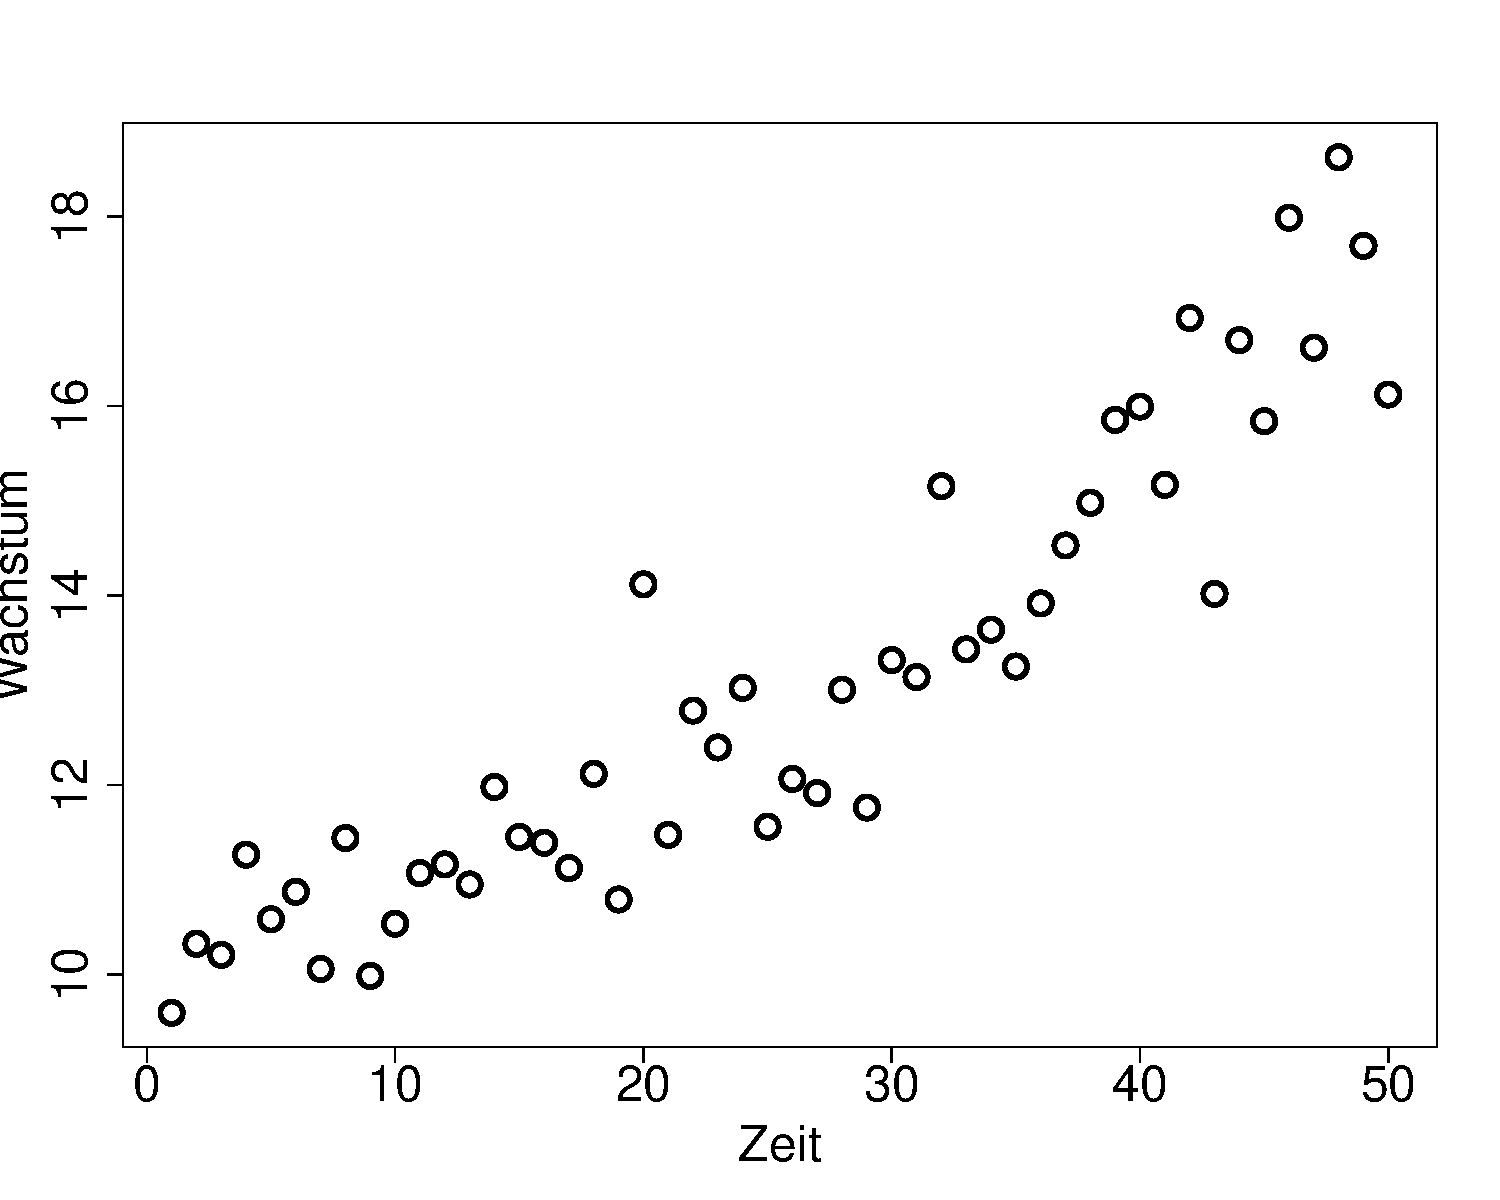
\includegraphics[width=0.5\textwidth]{data-raw-R}
  \caption{Plot der Beispieldaten}
  \label{Beispieldaten}
\end{figure}

In den folgenden Kapiteln wird mit einem normierten $Y$ gearbeitet, indem $Y$ durch $\max(Y)$ geteilt wird. Dadurch erhält man Werte zwischen Null und Eins, wodurch sich die Berechnungen vereinfachen.

Man kann die Daten normieren, da von 

\begin{equation*}
Y=X\beta+e
\end{equation*}

ausgehend, man zu 

\begin{equation*}
\tilde{Y} := \max(Y)^{-1} Y = X \max(Y)^{-1} \beta + \max(Y)^{-1} e =: X \tilde{\beta} + \tilde{e}
\end{equation*}

gelangt und dieses Modell immer noch multipel linear und homoskedastisch ist. 

Man kann ohne Einschränkung der Allgemeinheit davon ausgehen, dass die Elemente von $X$ Werte in $[0,1]$ annehmen. Sind die Werte nicht in $[0,1]$ kann man mit $\max(X)$ normieren.

Insgesamt erhält man aus $\tilde{\beta}$ wieder $\beta$ indem man mit $\max(Y)$ multipliziert.  

Benutzt man die Formeln \eqref{beta} und \eqref{sigma} von oben erhält man  $\hat{\beta}$ = \betaoneest ~und $\widehat{\sigma^2}$ = \sigmaoneest. In der Abbildung \ref{Beispieldaten_Regressionsgerade} sind die Daten mit der Regressionsgerade eingezeichnet.

\begin{figure}[H] 
  \centering
     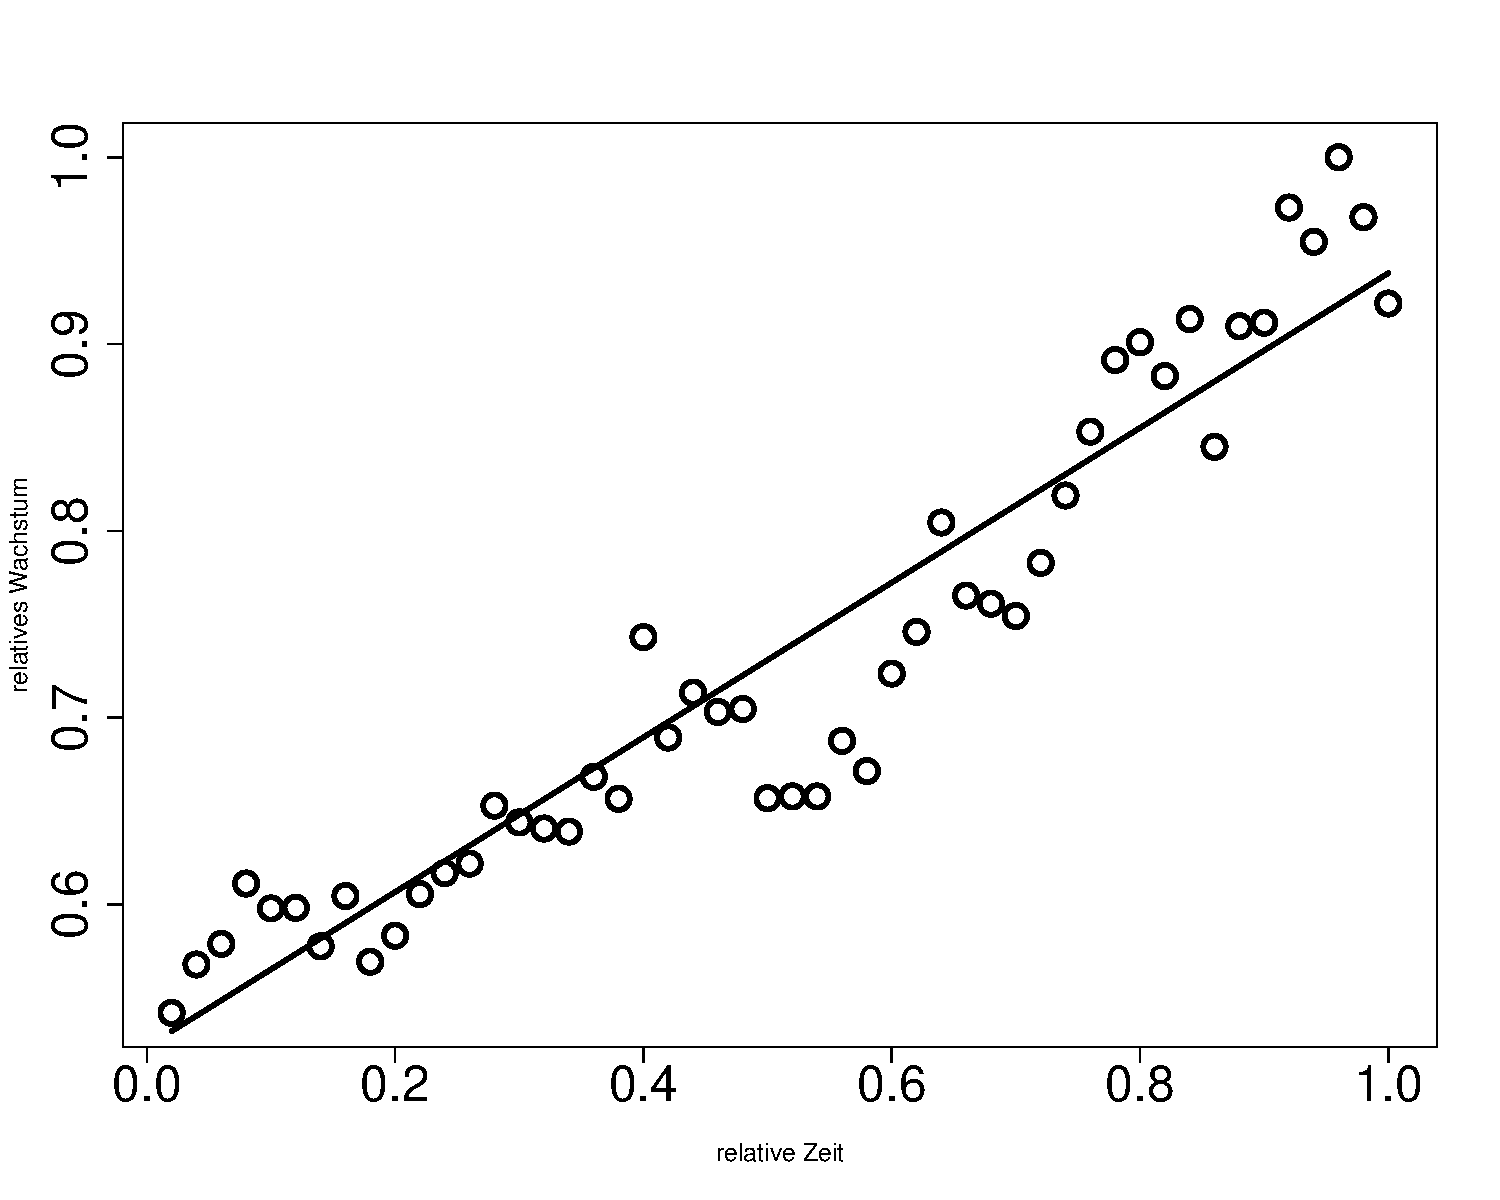
\includegraphics[width=0.5\textwidth]{regression-gerade}
  \caption{Plot der Beispieldaten mit Regressionsgerade}
  \label{Beispieldaten_Regressionsgerade}
\end{figure}
 
\end{Beispiel} 

Transferiert man die Schätzwerte mittels Multiplikation mit $\max(Y) = $ \maxY wieder zurück erhält man $\hat{\beta} =$ \betaesttrafo als Schätzer für $\beta =$ \betatrue ~und $\hat{\sigma} = $ \sigmaesttrafo ~als Schätzer für $\sigma = $ \sigmatrue .


\subsection{Konfidenzbänder}
\label{Konfidenzbaender}
In diesem Abschnitt werden Konfidenzbänder definiert und der Unterschied zwischen punktweisen und gleichmäßigen Konfidenzbändern wird erklärt. Die folgende Definition orientiert sich an \cite[229]{Georgii09}.

\begin{Definition}
Sei $( \chi, \mathscr{F} , \mathbb{P}_\vartheta : \vartheta \in \Theta) $ ein stochastisches Modell, $\Sigma$ eine beliebige Menge, $\tau : \Theta \rightarrow \Sigma $ eine zu ermittelnde Kenngröße für den Parameter $\vartheta$, und $0 < \alpha < 1$. Dabei bezeichnet \gls{P(...)} ein Wahrscheinlichkeitsmaß.

Eine Abbildung $C : \chi \rightarrow \mathscr{P}(\Sigma)$, die jedem möglichen Beobachtungsergebnis $x \in \chi$ eine Menge $C(x) \subset \Sigma$ zuordnet, heißt ein Konfidenz- oder Vertrauensbereich für $\tau$ zum Irrtumsniveau \gls{Wkeit} (beziehungsweise Sicherheitsniveau 1 - $\alpha$), wenn

\begin{equation*}
\inf_{\vartheta \in \Theta} \mathbb{P}_{\vartheta}(x \in \chi : C(x) \ni \tau(\vartheta)) \geq 1 - \alpha.
\end{equation*}

\end{Definition}

In dieser Ausarbeitung wird immer davon ausgegangen, dass $C(x)$ von der Form 

\begin{equation*}
C(x) = \Big \{ y \in \mathbb{R}^n :  x'\hat{\beta} - c ~ \hat{\sigma}\sqrt{x'(X'X)^{-1}x} \leq y \leq x'\hat{\beta} + c ~ \hat{\sigma}\sqrt{x'(X'X)^{-1}x} \Big \}
\end{equation*}

ist. Dabei ist \gls{kritischer-Wert} der sogenannte kritische Wert. Für den Rest der Ausarbeitung wird dies durch

\begin{equation*}
\mathbb{P} \left( x' \beta \in x'\hat{\beta} \pm c ~ \hat{\sigma}\sqrt{x'(X'X)^{-1}x} \right) = 1 - \alpha
\end{equation*} 

abgekürzt. Eine andere mögliche Schreibweise ist 

\begin{equation*}
\mathbb{P}(x'\beta \in M_n(x;Y,\alpha)) = x - \alpha
\end{equation*}

mit 

\begin{equation*}
M_n(x) = (x'\hat{\beta} -c, x'\hat{\beta} +c) 
\end{equation*}

und $c$ passend.

Weiterhin unterscheidet man punktweise und gleichmäßige Konfidenzbänder. Für punktweise Konfidenzbänder gilt für alle $x_{(0)} = (x_{1}, \ldots x_{p}) \in \mathbb{R}^p$

\begin{equation*}
\mathbb{P}(x'\beta \in x' \hat{\beta} \pm c) = 1-\alpha
\end{equation*}

während für gleichmäßige 

\begin{equation*}
\mathbb{P}(x'\beta \in x' \hat{\beta} \pm c ~ \text{ für alle } x_{(0)} \in \mathbb{R}^{p}) = 1-\alpha
\end{equation*}

gilt. Dabei ist $\beta=(\beta_{0}, \ldots, \beta_{p})$ der Koeffizientenvektor, der das Modell festlegt, und $\hat{\beta}$ ein Schätzer für $\beta$. 

In dieser Ausarbeitung werden nur gleichmäßige Konfidenzbänder betrachten.



%\begin{Beispiel}
%
%In der folgenden Abbildungen wird das Beispiel aus dem vorherigen Absatz um punktweise wie auch simultane Konfidenzbänder erweitert. Das punktweise Konfidenzband wurde mit \cite[15]{Liu64} bestimmt. Für das gleichmäßige Konfidenzband wurde die Methode aus dem nächsten Abschnitt verwendet.
%
%\begin{figure}[H] 
%  \centering
%     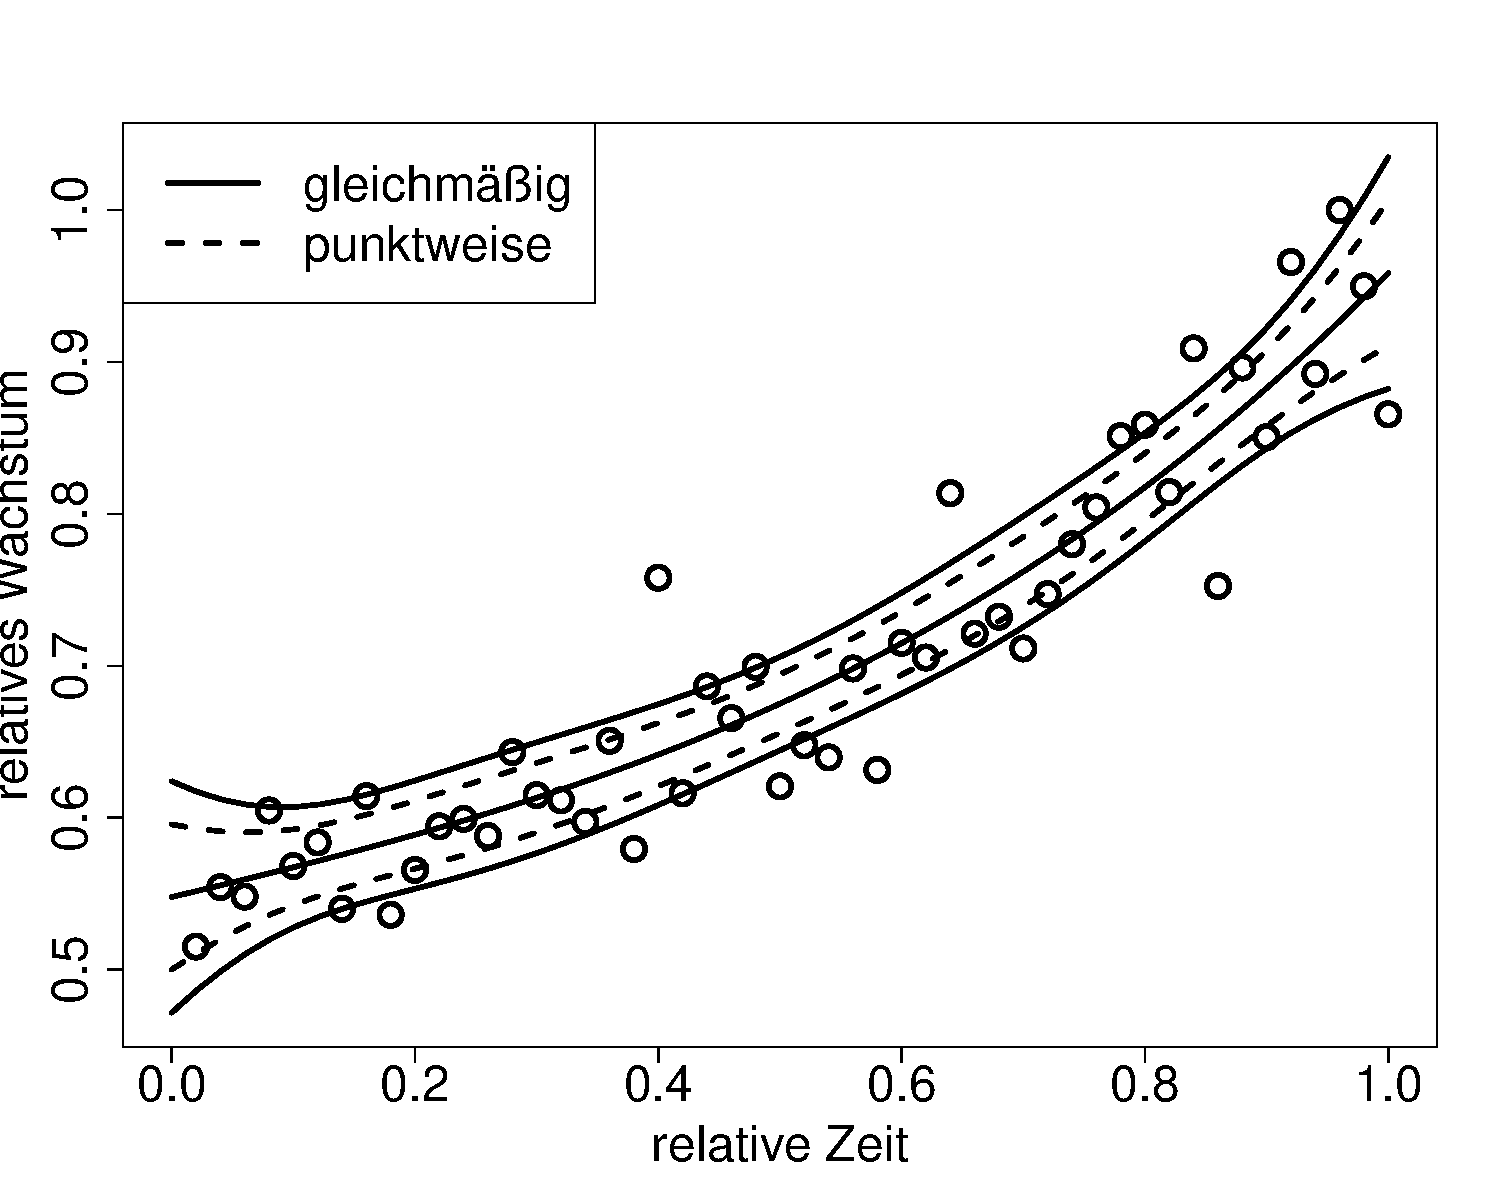
\includegraphics[width=0.5\textwidth]{punkt-vs-gleich}
%  \caption{Vergleich von punktweisen und gleichmäßigen Konfidenzbändern im Beispiel}
%  \label{punkt-vs-gleich_Beispiel}
%\end{figure}
%
%Man sieht, dass das gleichmäßige weiter ist, als das punktweise.
%
%\end{Beispiel}

 

\subsection{Konfidenzbänder auf $\mathbb{R}^{p}$ für ein multiples lineares Regressionsmodell}
\label{Konfidenzbaender auf R fuer ein multiples lineares Regressionsmodell}
Seien  $x,\beta, \hat{\beta}  \in \mathbb{R}^{p+1}$, $X \in \mathbb{R}^{n \times (p+1)}$. Wir gehen davon aus, dass $x = (1, x_{(0)}) \in \mathbb{R}^{p+1}$. In dem verbleibenden Teil dieses Kapitels werden Konfidenzbänder der Form

\begin{equation*} \label{KB_allgemein}
x' \beta \in x'\hat{\beta} \pm c ~ \hat{\sigma}\sqrt{x'(X'X)^{-1}x}
\end{equation*}

bestimmt. Dabei wird der kritische Parameter $c$ so gewählt, dass 

\begin{equation*}
\mathbb{P} \left( x' \beta \in x'\hat{\beta} \pm c \hat{\sigma}\sqrt{x'(X'X)^{-1}x} ~ \text{ für alle } x_{(0)} \in A \right) = 1-\alpha
\end{equation*}

gilt. Dabei ist $A$ ein Bereich, dem aus bestimmten Gründen besonderes Interesse gilt. Mehr zur Wahl von $A$ steht im nächsten Abschnitt. In diesem Abschnitt ist $A = \mathbb{R}^p$.

Wegen des folgenden Resultates aus \cite[66]{Liu64} benutzten wir diese Form von Konfidenzbändern.

\begin{Satz} \label{KB_Eigenschaft}
Für beliebiges $\beta \in \mathbb{R}^{p+1}$ und $\sigma > 0$ gilt 
\begin{equation*}
\mathbb{P} \left( x'\beta \in x' \hat{\beta} \pm \sqrt{(p+1) f^{\alpha}_{p+1,n-p-1}} \hat{\sigma} \sqrt{x' (X'X)^{-1}x} ~ \text{ für alle } x_{(0)} \in \mathbb{R}^p \right) = 1 - \alpha
\end{equation*}
Dabei ist \gls{f} das $\alpha$-Quantil der F-Verteilung mit Freiheitsgraden $p+1$ und $n-p-1$.
\end{Satz} 

Dieser Satz eröffnet uns eine einfache Möglichkeit, Konfidenzbänder auf $\mathbb{R}^p$ zu bestimmen. Da das Konfidenzband in Satz \ref{KB_Eigenschaft} von hyperbolischer Form ist, betrachteten wir in den folgenden Abschnitten immer hyperbolische Konfidenzbänder.

Um den Satz \ref{KB_Eigenschaft} beweisen zu können, brauchen wir die folgenden Resultate:

\begin{Lemma} \label{Basiseigenschaft}
Es ist
\begin{eqnarray*}
&&\mathbb{P} \left( x'\beta \in x' \hat{\beta} \pm c ~ \hat{\sigma} \sqrt{x' (X'X)^{-1} x} ~ \text{ für alle } x_{(0)} \in A \right) \\
&=& \mathbb{P} \left( \sup_{ x_{0} \in A} \bigg \vert \frac{x'(\beta - \hat{\beta})}{\hat{\sigma} \sqrt{x'(X'X)^{-1}x}} \bigg \vert \leq c \right) \\
&=& \mathbb{P}( S \leq c)
\end{eqnarray*}
mit 

\begin{equation*}
\sup_{x_{0} \in A} \frac{\vert x'(\beta - \hat{\beta}) \vert}{\hat{\sigma} \sqrt{x'(X'X)^{-1}x}}  =:  \gls{S}
\end{equation*}

\end{Lemma}

\begin{proof}
\begin{eqnarray*}
&& \mathbb{P} \left( x'\beta \in x' \hat{\beta} \pm c \hat{\sigma} \sqrt{x' (X'X)^{-1}x} ~ \text{ für alle } x_{(0)} \in A \right) \\
&=& \mathbb{P} \left( x' \hat{\beta} - c \hat{\sigma} \sqrt{x' (X'X)^{-1}x} \leq x'\beta \leq x' \hat{\beta} + c \hat{\sigma} \sqrt{x' (X'X)^{-1}x} ~ \text{ für alle } x_{(0)} \in A \right) \\
&=& \mathbb{P} \left( - c \hat{\sigma} \sqrt{x' (X'X)^{-1}x} \leq x' (\beta - \hat{\beta}) \leq  c \hat{\sigma} \sqrt{x' (X'X)^{-1}x} ~ \text{ für alle } x_{(0)} \in A \right) \\
&=& \mathbb{P} \left( - c  \leq \frac{x' (\beta - \hat{\beta})}{\hat{\sigma} \sqrt{x' (X'X)^{-1}x}}  \leq  c ~ \text{ für alle } x_{(0)} \in A \right) \\
&=& \mathbb{P} \left( \sup_{x_{0} \in A}  \frac{\vert x'(\beta - \hat{\beta}) \vert}{\hat{\sigma} \sqrt{x'(X'X)^{-1}x}}  \leq c \right)
\end{eqnarray*}
\end{proof}

Es geht in den folgenden Abschnitten immer darum, die Verteilung von $S$ zu bestimmen. Um diese Verteilung auf ganz $\mathbb{R}^p$ zu bestimmen, wird das folgende Ergebnis benutzt, welches sich an \cite[6]{Liu64} orientiert. 

\begin{Satz} \label{Basiseigenschaften}
Wenn Modell \eqref{Grundmodell_Regression} homoskedastisch ist, gilt mit Satz \ref{erster Satz} 

\begin{enumerate}
\item $\hat{\beta} \sim \mathscr{N}_{p+1}(\beta,\sigma^2(X'X)^{-1})$. Dabei ist $\mathscr{N}_{p+1}(\beta,\sigma^2(X'X)^{-1})$ die ($p$+1)-dimensionale Normalverteilung mit Erwartungswert $\beta$ und Kovarianzmatrix $\sigma^2 (X'X)^{-1}$.
\item $\hat{e} \sim \mathscr{N}_{n}(0,\sigma^2(I-H)) $ mit  \gls{H} $=X(X'X)^{-1}X' $
\item $\hat{\sigma}^2 \sim \frac{\sigma^2}{n-p-1}\chi_{n-p-1}^2 = \frac{\sigma^2}{v}\chi^2_{v}$. Dabei ist $n-p-1 := \gls{v}$, was auch im Verlauf dieser Ausarbeitung so beibehalten wird. Weiterhin ist \gls{chi-square} die Chi-Quadrat-Verteilung mit $v$ Freiheitsgraden.
\item $\hat{\beta}$ und $\widehat{\sigma^2}$ sind unabhängig.
\end{enumerate}
\end{Satz}

\begin{proof}
\begin{enumerate}
\item Benutzt man Modell \eqref{Grundmodell_Regression} und die Voraussetzung $ e \sim \mathscr{N}_{n}(0,\sigma^2 I_n)$, so folgt $Y=X \beta + e \sim \mathscr{N}_{n}(X\beta,\sigma^2 I_n)$. Da aus \eqref{beta} folgt, dass $\hat{\beta} = (X'X)^{-1} X' Y$ gilt, ist $\hat{\beta}$ eine Linearkombination von $Y$. Daraus folgt, dass auch $\hat{\beta}$ normalverteilt ist. Es genügt also den Erwartungswert und die Kovarianz zu bestimmen. 

\begin{align*}
\mathbb{E}(\hat{\beta}) = \mathbb{E}((X'X)^{-1}X'Y) = (X'X)^{-1} X' \mathbb{E}(Y) = (X'X)^{-1} X'X \beta = \beta
\end{align*}

und

\begin{eqnarray*}
\text{Cov}(\hat{\beta}) &=& \text{Cov}((X'X)^{-1} X' Y) = ((X'X)^{-1}X') \text{Cov}(Y) (X(X'X)^{-1}) \\
&=& ((X'X)^{-1}X') \sigma^2 I (X(X'X)^{-1}) = \sigma^2 (X'X)^{-1}
\end{eqnarray*}


\item Da nach \eqref{e} gilt, dass $\hat{e}=(I-H)Y$, ist $\hat{e}$ auch eine Linearkombination von Elementen aus $Y$. Da $Y$ normalverteilt ist, ist es also auch $\hat{e}$. Berechnet man wieder Erwartungswert und Kovarianz, erhält man:

\begin{eqnarray*}
\mathbb{E}(\hat{e}) &=& \mathbb{E}((I-H)Y) = (I-H)\mathbb{E}(Y) = (I-H)X\beta \\ 
&=& (I-X(X'X)^{-1}X')X = X-X(X'X)^{-1}X'X = X-X = 0
\end{eqnarray*}

und

\begin{align*}
\text{Cov}(\hat{e}) = \text{Cov}((I-H)Y) = (I-H) \text{Cov}(Y) (I-H) = \sigma^2 (I-H)
\end{align*}

Bei dieser Berechnung wird benutzt, dass die Matrix $I-H$ sowohl symmetrisch als auch idempotent ist. 

Die Matrix $I-H$ ist symmetrisch, da $H=X'(X'X)^{-1}X$ symmetrisch ist. Weiterhin ist die Matrix idempotent, da

\begin{eqnarray*}
(I-H)^2 &=& (I-X(X'X)^{-1}X')(I-X(X'X)^{-1}X') \\
&=& I + X(X'X)^{-1} X'X(X'X)^{-1}X' - 2 X(X'X)^{-1}X' \\
&=& I - X(X'X)^{-1}X' - X(X'X)^{-1}X'+ x(X'X)^{-1}X' \\
&=& (I-H)
\end{eqnarray*}


\item Sei $Q=I-H$ mit $H = X (X'X)^{-1} X'$, dann ist $Q$ symmetrisch und idempotent. Daraus folgt

\begin{eqnarray*}
\text{Rang}(Q) &=& \text{Spur}(Q) = \text{Spur}(I) - \text{Spur}(H) \\
		&=& n - \text{Spur}(X(X'X)^{-1}X') = n - \text{Spur}((X'X)^{-1}X'X) \\
		&=& n - (p+1)
\end{eqnarray*}

Dabei benutzt man $\text{Spur}(AB) = \text{Spur}(BA)$ . 

Also kann man $Q$ ausdrücken als $ Q = T' L T$. Dabei ist $T$ eine orthogonale Matrix und $L$ eine passende Diagonalmatrix mit den ersten $n-(p+1)$ Diagonalelementen Eins und den verbleibenden Diagonalelementen gleich Null.

Es ist $e=Y-X\beta \sim \mathscr{N}_{n}(0,\sigma^2 I_n)$. Sei $z=Te$. Dann ist $z\sim \mathscr{N}_{n}(0,\sigma^2 I_n)$, da aus der Orthogonalität von $T$ folgt, dass 

\begin{equation*}
\text{Var}(z) = \text{Var}(Te) = T \text{Var}(e) T' = T T' \text{Var}(\sigma^2 I_n) = I_n \sigma^2
\end{equation*}
. 

Weiterhin ist 

\begin{eqnarray*}
Qe = (I-H) (Y-X\beta) = (I-H)Y - (I-H)X \beta = (I-H)Y = \hat{e}
\end{eqnarray*}

da $(I-H)X=0$, wie oben bereits berechnet. Es folgt

\begin{eqnarray*}
\Vert \hat{e} \Vert^2 &=& \Vert Qe \Vert^2 = e'Q'Qe = e'Qe = (Te)' L (Te) \\
&=& z_1^2 + \ldots + z_{n-p-1}^2 \sim \sigma^2 \chi_{n-p-1}^2
\end{eqnarray*}

Setzt man dies nun in Gleichung \eqref{sigma}, das heißt $ \hat{\sigma}^2 = \Vert \hat{e} \Vert^{2} / (n-p-1) $, ein, erhält man 

\begin{equation*}
\hat{\sigma}^2 = \Vert \hat{e} \Vert^{2} / (n-p-1) \sim \frac{\sigma^2}{n-p-1} \chi_{n-p-1}^2
\end{equation*}


\item Da $\hat{\beta}$ und $\hat{e}$ normalverteilt sind, reicht es für die Behauptung der Unabhängigkeit zu zeigen, dass die Kovarianz zwischen den Beiden Null ist.

\begin{eqnarray*}
\text{Cov}(\hat{\beta},\hat{e}) &=& \text{Cov}((X'X)^{-1} X' Y, (I-H)Y) \\
&=& (X'X)^{-1} X' \text{Cov}(Y,Y) (I-H) \\
&=& \sigma^2 (X'X)^{-1} X' (I-H) \\
&=& \sigma^2 (X'X)^{-1} ((I-H)'X'')' \\
&=& \sigma^2 (X'X)^{-1} ((I-H) X)' = \sigma^2 (X'X)^{-1} 0 = 0
\end{eqnarray*}

\end{enumerate}
\end{proof}

Da wir nun von allen Bausteinen von $S$ die Verteilung kennen, können wir den Satz \ref{KB_Eigenschaft} beweisen. Satz und Beweis orientiert sich an \cite[66]{Liu64}.

\begin{proof}
Zu zeigen war, dass für beliebiges $\beta \in \mathbb{R}^{p+1}$ und $\sigma > 0$  im homoskedastischen Fall

\begin{equation*}
\mathbb{P} \left( x'\beta \in x' \hat{\beta} \pm \sqrt{(p+1) f^{\alpha}_{p+1,n-p-1}} \hat{\sigma} \sqrt{x' (X'X)^{-1}x}) ~ \text{ für alle } x_{(0)} \in \mathbb{R}^{p} \right) = 1 - \alpha
\end{equation*}

gilt. 

Sei \gls{P} die eindeutige Wurzel aus $(X'X)^{-1}$ und somit $(X'X)^{-1} = P^2$. Definiere außerdem, dass \gls{N} := $P^{-1}(\hat{\beta}-\beta)/\sigma$. Dann folgt $N$ einer ($p$+1)-dimensionalen Normalverteilung. Man hat also $N \sim \mathscr{N}_{p+1}(0,I_n)$ . 

Damit gilt
\begin{eqnarray*}
&&\mathbb{P} \left( x'\beta \in \sqrt{(p+1) f^{\alpha}_{p+1,n-p-1}} \hat{\sigma} \sqrt{x'(X'X)^{-1}x} ~ \text{ für alle } x_{(0)} \in \mathbb{R}^{p} \right) \\ 
&=& \mathbb{P} \left( \sup_{x_{(0)} \in \mathbb{R}^{p}} \frac{|x'(\hat{\beta}-\beta)|}{\hat{\sigma} \sqrt{x'(X'X)^{-1}x}} \leq \sqrt{(p+1) f^{\alpha}_{p+1,n-p-1}} \right) \\
&=& \mathbb{P} \left( \sup_{x_{(0)} \in \mathbb{R}^{p}} \frac{|(Px)'N|}{(\hat{\sigma}/\sigma)\sqrt{(Px)'(Px)}} \leq \sqrt{(p+1) f^{\alpha}_{p+1,n-p-1}} \right) \\
&=& \mathbb{P} \left( \frac{\parallel N \parallel}{(\hat{\sigma}/\sigma)} \left( \sup_{x_{(0)} \in \mathbb{R}^{p}} \frac{|(Px)'N|}{||Px|| ||N||} \right) \leq \sqrt{(p+1) f^{\alpha}_{p+1,n-p-1}} \right) \\
&=& \mathbb{P} \left(\frac{\parallel N \parallel}{(\hat{\sigma}/\sigma)} \leq \sqrt{(p+1) f^{\alpha}_{p+1,n-p-1}} \right) \\
&=& \mathbb{P} \left(\frac{(\hat{\beta}-\beta)'(X'X)(\hat{\beta}-\beta)}{(p+1)\hat{\sigma}^2} \leq f^{\alpha}_{p+1,n-p-1} \right) \\
&=& 1 - \alpha
\end{eqnarray*}

Dabei wird im vorletzten Schritt  die Cauchy-Schwarz-Ungleichung $ \vert (Px)'N \vert \leq \Vert Px \Vert \Vert N \Vert $ verwendet. Gleichheit gilt, falls $P x = \lambda N$ für ein $N$. 

Im letzten Schritt wird aus Satz \ref{Basiseigenschaften} benutzt, dass sowohl $(\hat{\beta}-\beta)'(X'X)(\hat{\beta}-\beta)$ als auch $(p+1)\hat{\sigma}^2$ einer $\chi^2$-Verteilung folgen. Außerdem sind beide unabhängig und somit ist ihr Quotient F-verteilt.

\end{proof}

\begin{Beispiel}
In der Abbildung \ref{KB-ganz-R-BSP} sind die Daten aus dem letzten Beispiel wieder mit einer polynomiellen Regression vom Grad Drei eingezeichnet.

Diesmal wird dazu noch ein Konfidenzband auf ganz $\mathbb{R}^{p}$ eingezeichnet. Die Berechnung ist in dem Verzeichnis \textit{/man/Beispiel-R.R} zu finden. Der kritische Parameter für dieses Konfidenzband ist \cR.

\begin{figure}[H] 
  \centering
     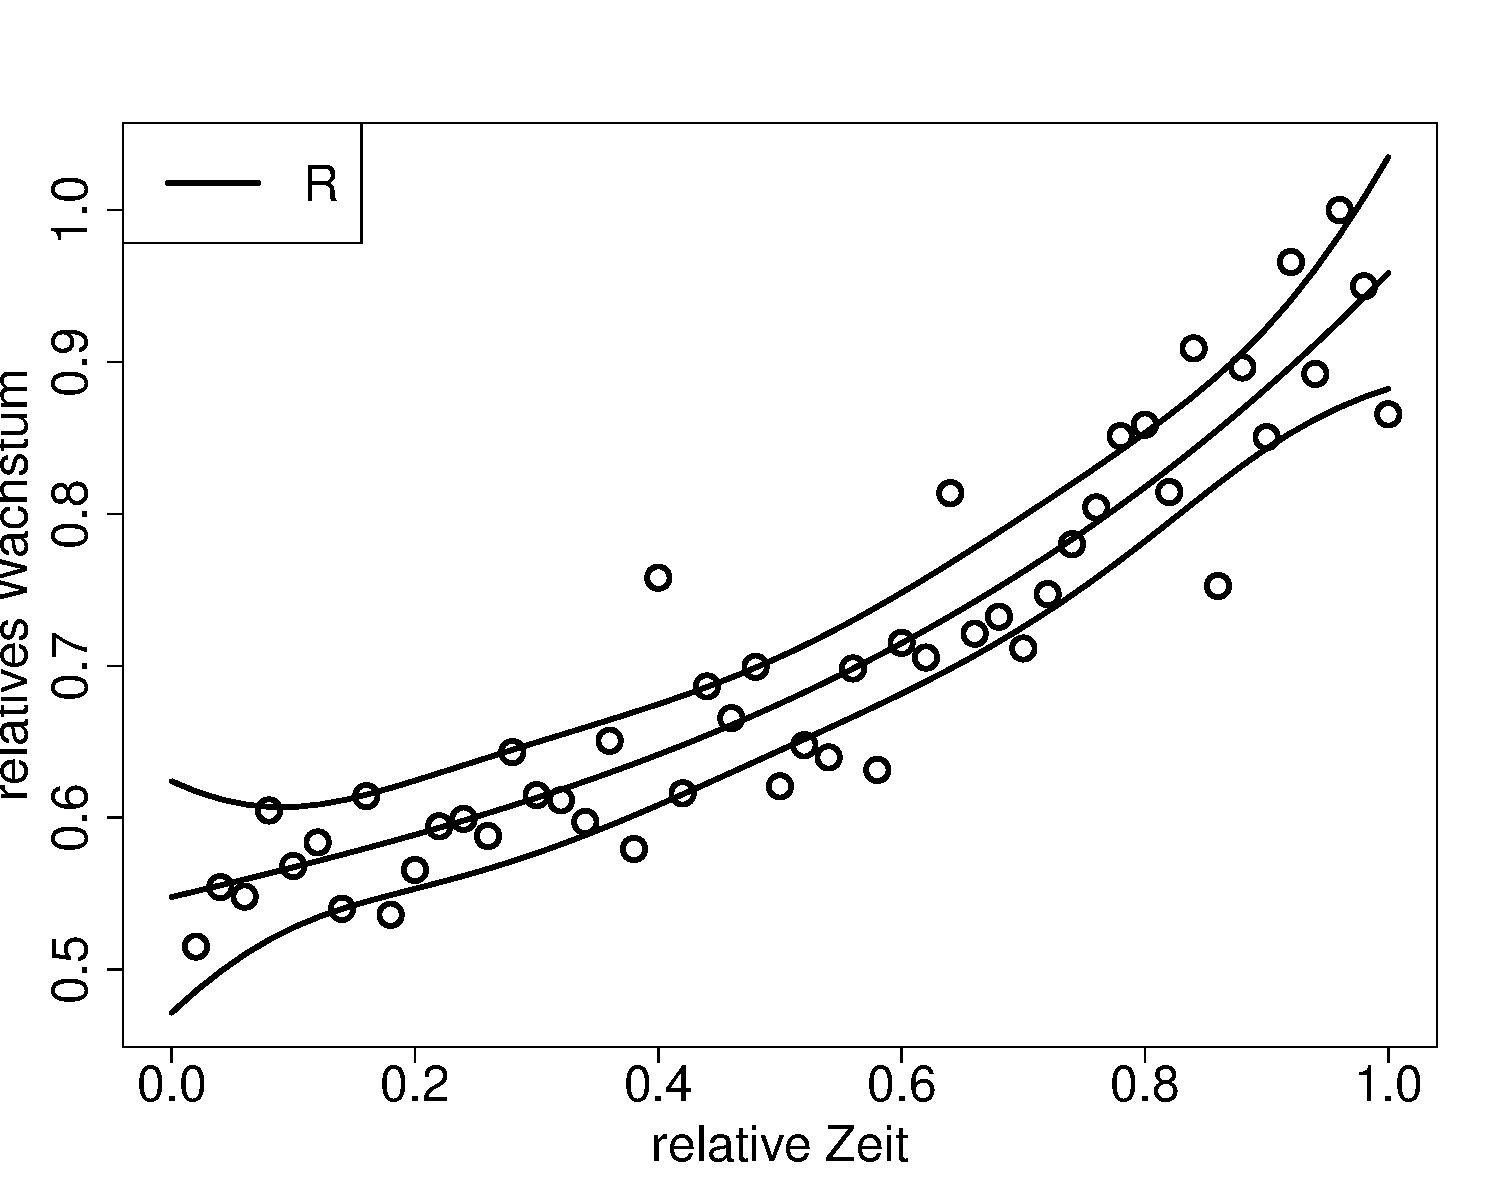
\includegraphics[width=0.5\textwidth]{Bsp-KB-R}
  \caption{Weiterführung des Beispiels durch Konfidenzband auf ganz $\mathbb{R}^{p}$}
  \label{KB-ganz-R-BSP}
\end{figure}

\end{Beispiel}

\begin{Simulation}
Außerdem wurde eine Simulation durchgeführt, um die Überdeckungswahrscheinlichkeit der Methode zu überprüfen.

Dazu wurden Daten auf zwei verschiedene Arten erzeugt. Zum Einen wurden die Daten auf Grundlage eines  multiplen, linearen, homoskedastisches Regressionsmodell erzeugt. Zum anderen wurde ein multiples lineares Regressionsmodell mit einem AR(1)-Prozess zugrunde gelegt. 

Der Grad des wahren Modelles ist \simgrad ~und es wird auch eine Regression mit Grad \simgrad ~durchgeführt. Dabei sind sowohl das wahre, als auch das geschätzte Modell von Polynomgestalt.

Bei der Simulation wurden zuerst \ntest ~Mal Daten mit den oben genannten Grundmodellen erzeugt. Danach wurden Konfidenzbänder um ein OLS-Schätzer beziehungsweise mit einem AR(1) transformierten OLS-Schätzer berechnet. Dann wurde gezählt, wie oft das wahre Modell in dem Konfidenzband lag. 

Für das multiple lineare Regressionsmodell kamen keine guten Werte bei den Überdeckungswahrscheinlichkeiten heraus. Deswegen wurde ein vereinfachtes Modell verwendet. Dabei wurde der Grad des Modells verringert, der Fehler auf 0.5 fixiert und die Anzahl an Beobachtungen erhöht. Außerdem wurde die Überdeckungswahrscheinlichkeit auf drei Stellen nach dem Komma genau bestimmt. Für nähre Informationen zu diesem Modell siehe das R Skript \textit{make-test-data-R.R}. Für das AR-Modell siehe das Skript \textit{make-test-data-AR.R}.

Auf Grund von Laufzeitproblemen werden die Daten von den Funktionen \textit{make-test-data-R} beziehungsweise \textit{make-test-data-AR} erzeugt und gespeichert. Auch die jeweils berechneten Regressionsmodelle, Designmatritzen und weitere Werte werden abgespeichert. Diese Daten sind in \textit{/data} zu finden.

Bei der Berechnung der Überdeckungswahrscheinlichkeit müssen dann nur noch die Konfidenzbänder, die von der Anzahl an Simulationen abhängen, berechnet werden. Für eine Erklärung warum Simulationen benötigt werden, siehe die Kapitel \ref{Konfidenzbaender auf R fuer ein multiples lineares Regressionsmodell} und \ref{Konfidenzbaenderauf auf einem Intervall für Regressionsmodell mit Polynomgestalt}.

Die Laufzeit für die Berechnung der Überdeckungswahrscheinlichkeiten von Konfidenzbänden bei denen Simulationen durchgeführt werden müssen beträgt ungefähr 15 Minuten bei den empfohlenen 5000 Wiederholungen.

Wie genau bei einem AR(1) Modell OLS-Schätzer bestimmt werden können wird in Kapitel \ref{Regression und Konfidenzbänder für abhaengige Daten} erläutert.

Die Ergebnisse sind in der folgenden Tabelle zusammengestellt:

\begin{center}
\begin{tabular}{|c|c|c|c|}
\hline 
 & unabhängig & AR bekannt & AR \\ 
\hline 
Konfidenzband auf ganz $\mathbb{R}^{p}$		 & \UeberRR		  & \UeberARbekanntR & \UeberARR \\ 
\hline 
\end{tabular} 
\end{center}

Die erste Spalte gibt die Überdeckungswahrscheinlichkeit bei dem homoskedastischen Modell an und die zweite bei einem AR(1)-Grundmodell mit bekanntem Korrelationsparameter. Bei der dritten Spalte ist dieser Parameter unbekannt und muss zusätzlich geschätzt werden. 

Man sieht, dass bei dieser Methode die Überdeckungswahrscheinlichkeit über der geforderten Wahrscheinlichkeit von 0.95 liegt. Der Grund dafür ist, dass das Konfidenzniveau auf ganz $\mathbb{R}^{4}$ eingehalten wird und nicht nur auf dem Intervall [0,1]. Für nähere Informationen dazu siehe Kapitel \ref{Konfidenzbaenderauf auf einem Intervall für Regressionsmodell mit Polynomgestalt}.

Diese Tabelle wird um weitere Zeilen mit den anderen Methoden Konfidenzbänder zu erzeugen erweitert, nachdem die neuen Methoden eingeführt worden sind.

\end{Simulation}



\subsection{Konfidenzbänder auf einem Intervall für ein einfaches lineares Regressionsmodell}
\label{Konfidenzbänder auf einem Intervall für ein einfaches lineares Regressionsmodell}
Dieser Abschnitt orientiert sich an \cite[17-23]{Liu64} und \cite{Liu08} und \cite{Wynn71}.

Für den Fall, dass wir nur eine unabhängige Variable $x_1$ haben, vereinfacht sich das Konfidenzband aus Gleichung \eqref{KB_allgemein} zu

\begin{equation}\label{simple_KB}
\mathbb{P} \left( \beta_0 + \beta_1 x_1 \in \hat{\beta_0} + \hat{\beta_1} x_1 \pm c \hat{\sigma} \sqrt{\nu(1,x_1)}  \text{ für alle } x_1 \in (a,b) \right)
\end{equation}

Dabei und für diesen Abschnitt gelten die folgenden Definitionen

\begin{eqnarray*}
\beta &:=& (\beta_0, \beta_1)' \\
\hat{\beta} &:=& (\hat{\beta_0}, \hat{\beta_1})' \sim \mathscr{N}_2(\beta, \sigma^2 (X'X)^{-1}) \\
P^2 &:=& (X'X)^{-1} \\
N &:=& P^{-1} (\hat{\beta} - \beta)/\sigma \sim \mathscr{N}_{2}(0,I_2) \\
T &:=& N / (\hat{\sigma} / \sigma) = P^{-1} (\hat{\beta}-\beta) / \hat{\sigma} \\
v &:=& n-2 \\
x_1 &:=& x \\
\nu(c,d) &:=& (c,d) (X'X)^{-1} (c,d)' \\
A &:=& (a,b)
\end{eqnarray*}

In \cite[19-20]{Liu64} wird folgendes Ergebnis gezeigt

\begin{eqnarray*}
&& \mathbb{P} \left( \beta_0 + \beta_1 x \in \hat{\beta_0} + \hat{\beta_1} x \pm c \hat{\sigma} \sqrt{\nu(1,x)}  \text{ für alle } x \in (a,b) \right)  \\
&=& \mathbb{P} \left( \sup_{x \in (a,b)} \vert (1,x) ( \hat{\beta} - \beta ) / \hat{\sigma} \vert / \sqrt{\nu(1,x)} < c \right) \\
&=& \mathbb{P} \left( \sup_{x \in (a,b)} \vert (P \cdot (1,x)')' \cdot T \vert / \Vert P \cdot (1,x)' \Vert < c \right) \\
&=& \mathbb{P} \left( T \in R_{h,2} \right)
\end{eqnarray*}

dabei ist

\begin{equation*}
R_{h,2}(x) = \{ T : \vert (P \cdot (1,x)' )' \cdot T \vert / \Vert P \cdot (1,x)' \Vert < c \}
\end{equation*}

eine Region von der Form $(T : \vert v'T \vert / \Vert v \Vert < r) \subset \mathbb{R}^2$. Deswegen kann man den Winkel $\phi$ zwischen den Vektoren $P \cdot (1,a)'$ und $P \cdot (1,b)'$ mittels

\begin{eqnarray*}
\cos \phi &=& (P \cdot (1,a)')' (P \cdot (1,b)') / \Vert P \cdot (1,a)' \Vert \Vert P \cdot (1,b)' \Vert \\
&=& (1,a) (X'X)^{-1} (1,b)' / \sqrt{\nu(1,a) \nu(1,b)} 
\end{eqnarray*}

berechnen. Jetzt folgt mit \cite{Wynn71}, dass gilt
%
%\begin{equation*}
%\mathbb{P}( \Vert T \Vert < c ) = \mathbb{P}(R_T < c) = 1 - (1+c^2/\nu)^{-\nu/2}
%\end{equation*}
%
%außerdem hat man
%
%\begin{eqnarray*}
%\frac{2}{\pi} \int^{(\pi-\phi)/2}_{0} \biggl( \bigl( 1 + \frac{c^2}{\nu} \bigr)^{-\nu/2} - \bigl( 1 + \frac{c^2}{\nu \sin^2(\phi + \phi/2)} \bigr)^{-\nu/2} \biggr) \text{d} \phi
%\end{eqnarray*}


\begin{eqnarray*}
\mathbb{P} \left( \beta_0 + \beta_1 x \in \hat{\beta_0} + \hat{\beta_1} x \pm c \hat{\sigma} \sqrt{\nu(1,x)} \text{ für alle } x \in (a,b) \right) \\
= 1 - \frac{\phi}{\pi} \biggl( 1 + \frac{c^2}{v} \biggr)^{ - v/2} - \frac{2}{\pi} \int^{(\pi - \phi)/2}_{0} \biggl( 1 + \frac{c^2}{v \sin^2(\theta + \phi/2)} \biggr)^{-v/2} \text{d} \theta
\end{eqnarray*}

Man muss also 

\begin{equation*}
1 - \frac{\phi}{\pi} \biggl( 1 + \frac{c^2}{v} \biggr)^{ - v/2} - \frac{2}{\pi} \int^{(\pi - \phi)/2}_{0} \biggl( 1 + \frac{c^2}{v \sin^2(\theta + \phi/2)} \biggr)^{-v/2} \text{d} \theta = 1 - \alpha
\end{equation*}

nach $c$ lösen und kann dann das Konfidenzband \eqref{simple_KB} bestimmen.





\subsection{Konfidenzbänder auf einem Intervall für ein multiples lineares Regressionsmodell}
\label{Konfidenzbaender auf einem Intervall fuer ein multiples lineares Regressionsmodell}
Im Abschnitt \ref{Konfidenzbaender auf R fuer ein multiples lineares Regressionsmodell} wurden Konfidenzbänder auf ganz $\mathbb{R}^p$ konstruiert. Allerdings kann es bei der Verwendung einiger unabhängigen Variablen nicht sinnvoll sein, das Konfidenzband auf ganz $\mathbb{R}^{p}$ zu konstruieren. Ist die unabhängige Variable zum Beispiel ein Gewicht, reicht es, ein Konfidenzband auf $\mathbb{R}_{+}^{p}$ zu konstruieren. Schließlich sind Gewichte immer positiv.

Nachfolgend wird das uns interessierende Gebiet mit $A$ bezeichnet. Dabei ist 

\begin{equation*}
A = \{(x_1, \ldots, x_p)' : a_i \leq x_i \leq b_i, i = 1, \ldots, p \} \subset \mathbb{R}^p \text{ für } - \infty \leq a_i < b_i \leq \infty, i=1, \ldots, p
\end{equation*}

Außerdem definieren wir $x_{(0)} := (x_1, \ldots, x_p)'$.

Eine Möglichkeit, ein Konfidenzband auf $A$ zu bestimmen, ist, ein Konfidenzband auf ganz $\mathbb{R}^p$ zu konstruieren und dann den Teil auf $\mathbb{R}^{p} \setminus A$ zu vernachlässigen.

Da dann die Bedingung $\mathbb{P}(x'\beta \in x' \hat{\beta} \pm d ~ \text{ für alle } x_{(0)} \in A) = 1-\alpha$ für mehr $x_{(0)}$-Werte als nötig erfüllt sein muss, ist das Konfidenzband dann weiter, als es sein müsste. Dabei ist $d$ eine beliebig, aber fest gewählte Konstante.

Besser ist die folgende Möglichkeit, die sich an \cite[70]{Liu64} orientiert. Das Ziel ist wieder ein hyperbolisches Konfidenzband der Form 

\begin{equation}
x'\beta \in x' \hat{\beta} \pm c ~ \hat{\sigma} \sqrt{x' (X'X)^{-1}x} \label{hyperbolisches_KB}
\end{equation}

zu erzeugen, um es mit dem Band aus Abschnitt \ref{Konfidenzbaender auf R fuer ein multiples lineares Regressionsmodell} vergleichen zu können. Das Problem ist, ein geeignetes $c$ zu finden, sodass 

\begin{equation*}
\mathbb{P} \left( x'\beta \in x' \hat{\beta} \pm c ~ \hat{\sigma} \sqrt{x' (X'X)^{-1}x} ~ \text{ für alle } x_{(0)} \in A \right) = 1-\alpha
\end{equation*}
 
gilt.

Aus Satz \ref{Basiseigenschaft} aus Abschnitt \ref{Konfidenzbaender auf R fuer ein multiples lineares Regressionsmodell} ist bekannt, dass 

\begin{equation*}
\mathbb{P} \left( x'\beta \in x' \hat{\beta} \pm c ~ \hat{\sigma} \sqrt{x' (X'X)^{-1}x} ~ \text{ für alle } x_{(0)} \in A \right) = \mathbb{P}(S<c)
\end{equation*}

Dabei ist $S$ gegeben durch 

\begin{equation*}
S = \sup_{x_{(0)} \in A} \frac{\vert x'(\beta - \hat{\beta}) \vert}{\hat{\sigma} \sqrt{x'(X'X)^{-1}x}}
\end{equation*}

Da die Verteilung von $S$ nicht von $\beta$ und $\sigma^2$ abhängt, ist es in dieser Hinsicht ein Pivot\-element. Dabei ist $\beta$ wieder der Koeffizientenvektor und $\sigma^2$ die Varianz der Fehler. 

Um zu sehen, dass die Verteilung von $S$ nicht von $\beta$ und $\sigma^2$ abhängt, betrachte Satz \ref{Basiseigenschaften}. Dort wurde gezeigt, dass $\hat{\beta} \sim \mathscr{N}_{p+1}(\beta, \sigma^2 (X'X)^{-1})$ und $\hat{\sigma} \sim \sigma^2/(n-p-1) \cdot \chi^2_{n-p-1}$. Fügt man nun $1=\sigma / \sigma$ ein, folgt die Behauptung.

Allerdings hängt die Verteilung von $S$ immer noch in komplizierter Art und Weise von der Designmatrix $X$ und den Grenzen $a_i$ und $b_i$ von $A$ für $i=1, \ldots, p$ ab.

Seien $P$ und $N$ definiert wie im Beweis zu Satz \ref{KB_Eigenschaft}. Das heißt, 

\begin{eqnarray*}
P^2 &:=& (X'X)^{-1} \\
N &:=& \frac{P^{-1}(\hat{\beta}-\beta)}{\sigma}
\end{eqnarray*}

Dann hat 

\begin{equation*}
T = \frac{N}{(\hat{\sigma} /\sigma)} = \frac{P^{-1}(\hat{\beta}-\beta)}{\hat{\sigma}}
\end{equation*}

eine so genannte \gls{Tau} Verteilung. Damit kann man $S$ ausdrücken als

\begin{eqnarray*}
S &=& \sup_{x_{0} \in A} \frac{\vert(Px)'(P^{-1} (\hat{\beta}-\beta)) / \hat{\sigma} \vert}{\sqrt{(Px)'(Px)}}\\
&=& \sup_{x_{0} \in A} \frac{\vert (Px)' T \vert}{\Vert Px \Vert} \\
&=& \sup_{v \in C(P,A)} \frac{\vert v'T \vert}{\Vert v \Vert}
\end{eqnarray*}

mit 

\begin{eqnarray*}
C(P,A) &=& \{ \lambda P x : \lambda \geq 0, x \in A \} \\
&=& \{ \lambda (p_0+x_1 p_1 + \ldots +x_p p_p) : \lambda \geq 0, x_i \in [a_i,b_i] ~ \text{ für alle } i=1,\ldots,p \}
\end{eqnarray*}

wobei $P=(p_0, \ldots, p_p)$. 

Allerdings ist es für ein allgemeines $p \geq 1$ sehr schwierig, eine Formel für die Verteilung von $S$ explizit zu berechnen, um die kritische Konstante $c$ zu bestimmen \cite[S.70, Z.18]{Liu64}. Deswegen wird eine Simulation benutzt.

Man beachte, dass $C(P,A)$ der Kegel ist, der von den Vektoren $p_0+c_1 p_1 + \ldots + c_p p_p $ aufgespannt wird, wobei $c_i$ entweder $a_i$ oder $b_i$ für $i=1,\ldots,p$ ist. 

Sei \gls{Pi} die Projektion von $t \in \mathbb{R}^{p+1}$ auf den Kegel $C(P,A)$, d.h. $\pi(t,P,A)$ löst $ \min_{v \in C(P,A)} \Vert v-t \Vert$. Jetzt folgt mit \cite[Theorem 2.1]{Naiman87} , dass $S$ die Gleichung

\begin{equation*}
S=\max(\Vert \pi(t,P,A) \Vert, \Vert \pi(-t,P,A) \Vert)
\end{equation*}
 
löst. 

Man kann also die kritische Konstante $c$ mit folgender Simulation finden:

\begin{enumerate}
\item Simuliere $N \sim \mathscr{N}_{p+1}(0,I_{n})$ und $\hat{\sigma}/\sigma\sim\sqrt{\chi_v^2/v}$ mit $v=n-p-1$ und $p$ der Anzahl an unabhängigen Parametern.
\item Berechne $\pi(t,P,A)$ und $\pi(-t,P,A)$ .
\item Berechne $S=\max(\Vert \pi(t,P,A) \Vert, \Vert \pi(-t,P,A) \Vert)$ .
\end{enumerate}

Wiederholt man diese Schritte $k$ mal, so erhält man $S_1, \ldots, S_k$. Dann ist $c$ das $1-\alpha$ Quantil von $S_1, \ldots, S_k$.

Um $\pi(t,P,A)$ und $\pi(-t,P,A)$ zu bestimmen, wird folgendes Verfahren verwendet, das aus \cite[Appendix B]{Liu64} stammt:

Es soll das $v$ in $\mathbb{R}^{p+1}$, das $\Vert v-t \Vert^2$ minimiert, gefunden werden. Dabei soll $v \in C(P,A_{r})$ sein, mit $C(P,A_{r})$ wie oben definiert. 

Dazu betrachten wir

\begin{equation*}
\Vert v-t \Vert^2 = v'v-2t'v+t't 
\end{equation*}
%= (\frac{1}{2} v'v-t'v+\frac{1}{2} t't) \cdot 2

Man sieht, dass $t't$ unabhängig von $v$ ist. Deshalb muss man es bei der Minimierung von $\Vert v-t \Vert^2$ nicht berücksichtigen.
 
Sei $e_j \in \mathbb{R}^{p+1}$ der $j$-te Einheitsvektor. Aus der Definition von $C(P,A_{r})$ ist zu sehen, dass $v \in C(P,A_{r})$ impliziert, dass $v=\lambda P x$ oder gleichwertig $P^{-1}v=\lambda x = (\lambda, \lambda x_1, \ldots , \lambda x_p)'$ für ein $x \in A_{r}$ und $\lambda \geq 0$ gelten muss. Deshalb ist $e_1'P^{-1}v = \lambda \geq 0$ und $a_j \leq e_{j+1}'P^{-1}v/e_1'P^{-1}v = x_j \leq b_j$ für $j = 1, \ldots p$ oder gleichwertig

\begin{eqnarray*}
- e_1' P^{-1} v &\leq & 0 \\
(e_{j+1}' - b_j e_1') P^{-1} v &\leq & 0 ~~\text{ ,für } j = 1, \ldots, p \\
(a_{j} e_1' - e_{j+1}')P^{-1} v &\leq & 0 ~~\text{ ,für } j = 1, \ldots, p
\end{eqnarray*}

Diese Beschränkungen kann man zusammenfassen zu 

\begin{equation*}
A v \leq 0
\end{equation*}

wobei $A$ die $(2p+1) \times (p+1)$ Matrix

\[ 
A = 
\begin{bmatrix} (e_2'-b_1 e_1')P^{-1}  \\ 
				(a_1 e_1' - e_2')P^{-1}  \\  
				\ldots						 \\ 
				(e_{p+1}' - b_p e_1') P^{-1}	\\  
				(a_p e_1' - e_{p+1}')P^{-1}  \\
				-e_1'P^{-1} 
\end{bmatrix}
\]

ist. Für Minimierungsprobleme dieser Art gibt es ein R-Paket namens \textit{quadprog} , das zur Lösung dieser Minimierungsaufgabe benutzt wird.

\begin{Beispiel}
Jetzt wird das Beispiel aus Abschnitt \ref{Konfidenzbaender auf R fuer ein multiples lineares Regressionsmodell} fortgeführt, indem zu der Regression mit Grad Drei und dem Konfidenzband auf ganz $\mathbb{R}^{3}$ noch ein Konfidenzband auf $A$ eingezeichnet wird. Dabei benutzt man $A = \{x_{0} \in \mathbb{R}^3 : x_i \in [0,1] \text{ für alle } i=1, 2, 3 \} $. 


\begin{figure}[H] 
  \centering
     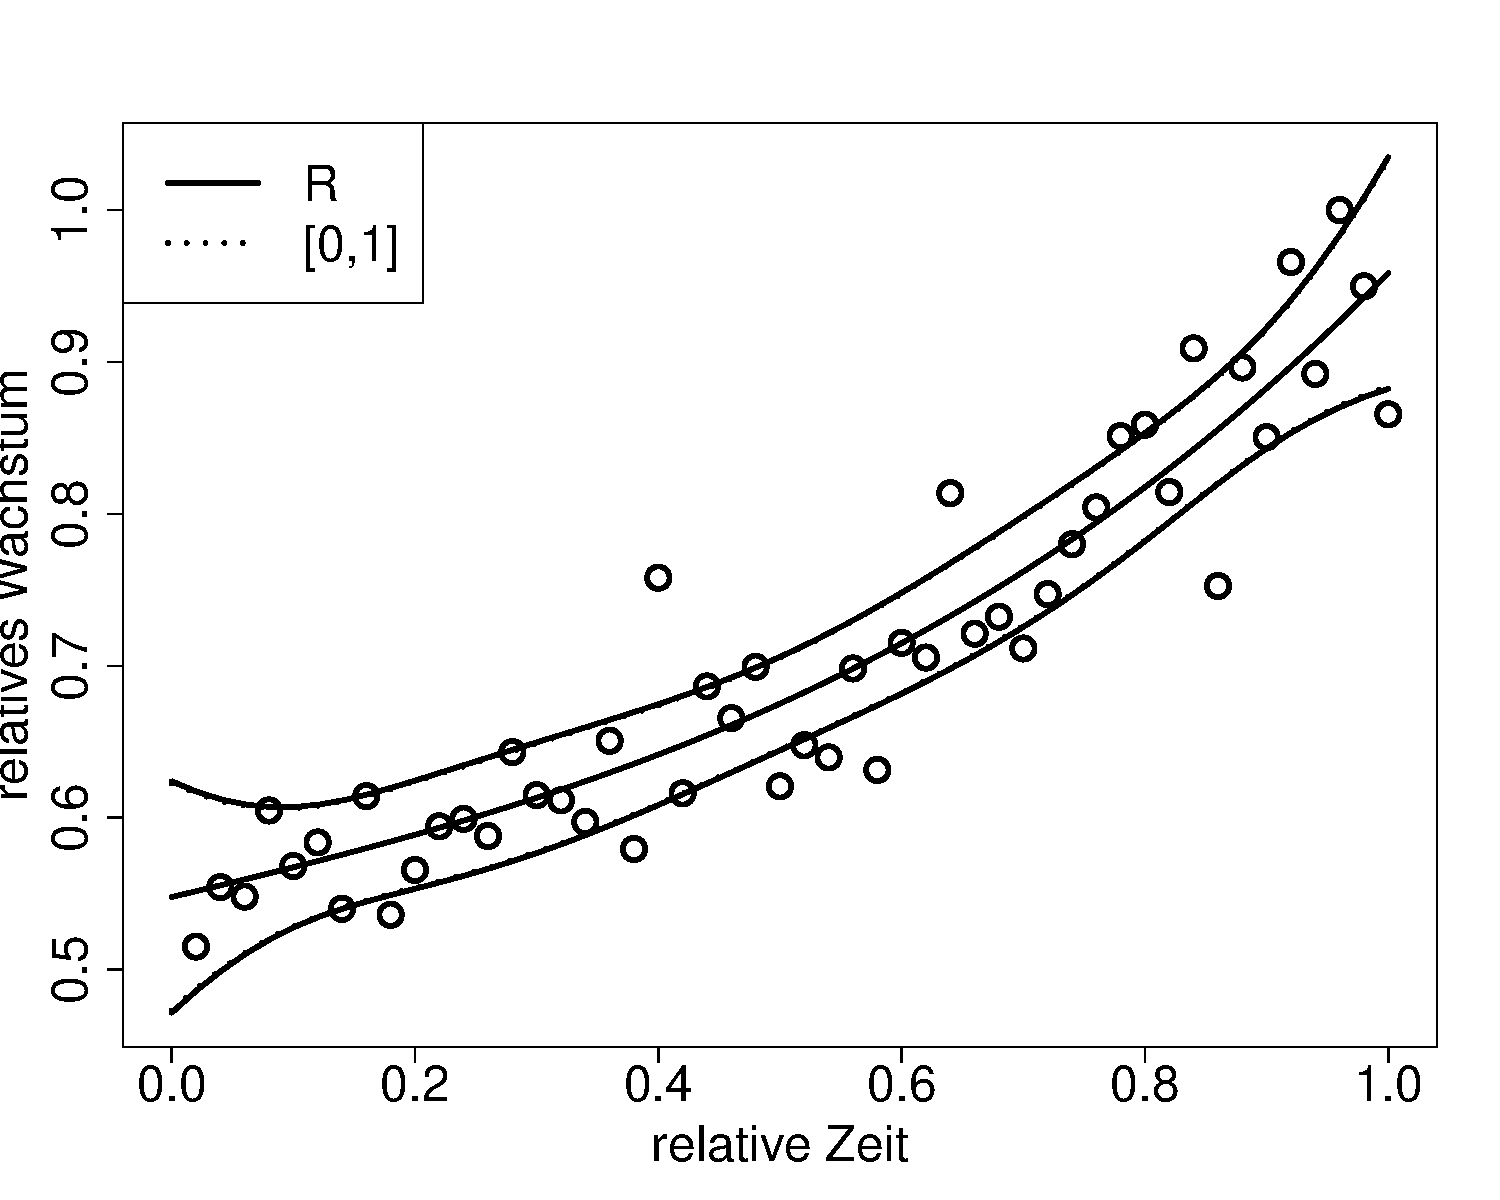
\includegraphics[width=0.5\textwidth]{Bsp-KB-minmax}
  \caption{Beispieldaten aus Kapitel \ref{Regression und Konfidenzbaender} mit einem Konfidenzband nach Kapitel \ref{Konfidenzbaender auf R fuer ein multiples lineares Regressionsmodell} und einem nach Kapitel \ref{Konfidenzbaender auf einem Intervall fuer ein multiples lineares Regressionsmodell}}
  \label{KB-minmax-BSP}
\end{figure}

Der kritische Wert für das Konfidenzband auf ganz $\mathbb{R}^3$, der bereits in Abschnitt \ref{Konfidenzbaender auf R fuer ein multiples lineares Regressionsmodell} berechnet wurde, ist \cR . Für das Konfidenzband auf $A$ ergibt sich \cA ~als kritischer Wert für das Konfidenzband. Dieser Wert ist kleiner als der bisherige, was auch zu erwarten war.

Dies sieht man auch daran, dass das Konfidenzband auf $A$ schmaler ist, als das Konfidenzband auf $\mathbb{R}^3$. 
\end{Beispiel}

\begin{Simulation}
Jetzt wird die Simulationstabelle aus dem Abschnitt \ref{Konfidenzbaender auf R fuer ein multiples lineares Regressionsmodell} durch Überdeckungswahrscheinlichkeiten für die Konfidenzbänder auf $A$ fortgesetzt. 

In diesem Fall ist $A = \{x \in \mathbb{R}^4 : x_i \in [0,1] \text{ für alle } i=1, 2, 3, 4 \}$. Dies liegt daran, dass wir die Matrix $X$ so wählen, dass die unabhängigen Variablen im Intervall $[0,1]$ liegen.

Die neuen Überdeckungswahrscheinlichkeiten für Konfidenzbänder auf Intervallen werden mit Minmax bezeichnet. Auch diese Überdeckungswahrscheinlichkeiten liegen über den geforderten 0.95.

\begin{center}
\begin{tabular}{|c|c|c|c|}
\hline 
 & unabhängig & AR bekannt & AR \\ 
\hline 
Konfidenzband auf ganz $\mathbb{R}^{p}$		 & \UeberRR		  & \UeberARbekanntR & \UeberARR \\ 
\hline 
Konfidenzband auf einem Polyeder	 & \UeberRMinmax  & \UeberARbekanntMinmax & \UeberARMinmax \\ 
\hline 
\end{tabular} 
\end{center}

\end{Simulation}


\newpage
\subsection{Konfidenzbänder auf auf einem Intervall für ein Regressionsmodell mit Polynomgestalt}
\label{Konfidenzbaenderauf auf einem Intervall für Regressionsmodell mit Polynomgestalt}
In diesem Abschnitt betrachten wir wieder das Regressionsmodell 

\begin{equation*}
Y=X\beta+e
\end{equation*}

mit $Y$ einem $1 \times n$ Datenvektor, $\beta$ ein $1 \times (p+1)$ Koeffizientenvektor und $e \sim \mathscr{N}_{n}(0,\sigma^2 I_n )$ ein $1 \times n$ Zufallsfehlervektor.

In den ersten Abschnitten lag die Annahme zugrunde, dass $X$ irgendeine feste, aber beliebige $n \times (p+1)$ Matrix ist. Im letzten Abschnitt sind wir zusätzlich implizit davon ausgegangen, dass die erste Spalte von $X$ nur mit Einsen besetzt ist.

In diesem Abschnitt betrachten wir den Fall, dass die Spalten von $X$ einen funktionalen Zusammenhang erfüllen. Konkret gehen wir davon aus, dass die $i$-te Zeile von $X$ von der Form $\tilde{x}_i = (1, x, x^{2}, \ldots, x^{p}) \in \mathbb{R}^{p+1}, i = 1, \ldots, n$ ist. 

Unsere Designmatrix ist also zeilenweise von Polynomgestalt. Dies ist genau der Fall, den wir im Beispiel und den Simulationen, die am Ende der Abschnitte stehen, betrachtet haben. 

Das Ziel ist wieder Konfidenzbänder der Form 

\begin{equation}
\tilde{x}' \beta \in \tilde{x}' \hat{\beta} \pm c \hat{\sigma} \sqrt{\tilde{x}'(X'X)^{-1}\tilde{x}} ~ \text{ für alle } x \in A=(a,b)
\end{equation}

zu bestimmen. Dann können wir sie direkt mit den Konfidenzbändern aus den Abschnitten \ref{Konfidenzbaender auf R fuer ein multiples lineares Regressionsmodell} und \ref{Konfidenzbaender auf einem Intervall fuer ein multiples lineares Regressionsmodell} vergleichen. Dazu reicht es nur die  die kritischen Konstanten $c$ miteinander zu vergleichen. 

Dabei ist die kritische Konstante $c$ wieder so zu bestimmen, dass

\begin{equation*}
\mathbb{P} \left( \tilde{x}' \beta \in \tilde{x}' \hat{\beta} \pm c \hat{\sigma} \sqrt{\tilde{x}'(X'X)^{-1} \tilde{x}} ~ \text{ für alle } x \in A=(a,b) \right) = 1 - \alpha
\end{equation*}

gilt. 

Es können allerdings nicht direkt die Ergebnisse aus dem letzten Abschnitt benutzen werden. Der Grund dafür sind die folgenden zwei Eigenschaften, die \cite[180]{Liu64} entnommen sind.

\begin{enumerate}
\item Angenommen es seien zwei seien zwei polynomiale Modelle $\tilde{x}' \beta_1$ und $\tilde{x}' \beta_2$ gegeben und das erste ist näher an dem wahren Modell als das zweite. Näher meint in diesem Fall, dass

\begin{align*}
\sup_{x \in \mathbb{R}} \frac{\vert \tilde{x}'(\hat{\beta_1} - \hat{\beta}) \vert}{\hat{\sigma} \sqrt{\tilde{x}'(X'X)^{-1}\tilde{x}}} < 
\sup_{x \in \mathbb{R}} \frac{\vert \tilde{x}'(\hat{\beta_2} - \hat{\beta}) \vert}{\hat{\sigma} \sqrt{\tilde{x}'(X'X)^{-1}\tilde{x}}}
\end{align*}

Zu erwarten ist, dass das erste Modell sinnvoll ist, wenn auch das zweite sinnvoll ist. Immerhin ist das erste Modell näher an dem wahren Modell, als das zweite.

Dies ist allerdings für die bisher betrachteten Konfidenzbänder nicht der Fall, da die bisher betrachteten Verfahren die spezielle polynomiale Struktur nicht berücksichtigen. 

\item Die kritische Konstante $c$ kann kleiner als im letzten Abschnitt gewählt werden. Der Grund dafür ist, dass das Konfidenzband nur auf einer Teilmenge 

\begin{equation*}
\{ \tilde{x} : \tilde{x}=(1,x,\ldots,x^p) \text{ für ein } x \in \mathbb{R}\} \subset \mathbb{R}^{p+1}
\end{equation*}

die Wahrscheinlichkeit $1-\alpha$ haben muss.
\end{enumerate}

Als Lösung wird in diesem Abschnitt eine Methode, die auf Simulation basiert, vorgestellt. Das Vorgehen ist also ähnlich zu dem Vorgehen in Abschnitt \ref{Konfidenzbaender auf einem Intervall fuer ein multiples lineares Regressionsmodell}. Diese Methode orientiert sich an \cite[183,184]{Liu64}.

Im Satz \ref{Basiseigenschaft} haben wir das Konfidenzniveau vom Modell $Y=X\beta+e$, mit $Y,X,\beta,e$ wie üblich, als $\mathbb{P}(S \leq c)$ bestimmt. Dabei ist

\begin{eqnarray*}
S &=& \sup_{x_{0} \in A} \frac{\vert \tilde{x}'(\hat{\beta}-\beta) /\hat{\sigma} \vert}{\sqrt{\tilde{x}'(X'X)^{-1}\tilde{x}}} \\
&=& \sup_{x_{0} \in A} \frac{|\tilde{x}'N/(\hat{\sigma}/\sigma)|}{\sqrt{\tilde{x}'(X'X)^{-1}\tilde{x}}} \\
&=& \sup_{x_{0} \in A} \frac{| \tilde{x}'T |}{\sqrt{\tilde{x}'(X'X)^{-1}\tilde{x}}} \\
&=& K_{2h}(T,(X'X)^{-1},(a,b))
\end{eqnarray*}

Man beachte, dass in diesem Fall $A=[a,b]$ mit $a,b \in \mathbb{R}$ gilt. Der Grund dafür ist, dass \gls{X-Tilde}$ = (1, x, x^2, \ldots, x^p)$ ist.

In den obigen Umformungen wurden die Definitionen $ N := (\hat{\beta}-\beta)/\sigma \sim \mathscr{N}_{p+1
} (0,(X'X)^{-1}) $ , \gls{T} := $N/(\hat{\sigma}/\sigma)\sim\tau_{p+1,v}(0,(X'X)^{-1}) $ und für \gls{K}

\begin{equation*}
K_{2h}(T;(X'X)^{-1};(a,b)) := \sup_{x_{0} \in A} \frac{|\tilde{x}'T|}{\sqrt{\tilde{x}'(X'X)^{-1}\tilde{x}}}
\end{equation*}

benutzt.
$f$
Es ist also klar, dass $c$ das $1-\alpha$ Quantil von $S = K_{2h}(T;(X'X)^{-1};(a,b))$ ist. Allerdings ist die Verteilung von $K_{2h}(T;(X'X)^{-1};(a,b))$ nur schwer explizit zu bestimmen.

Um $c$ trotzdem zu ermitteln, kann man $r$ unabhängige Realisationen von $S$ berechnen und von diesen $S_1, \ldots, S_r$ das $1-\alpha$ Quantil benutzen.

Um $S$ für vorgegebene $N$ und $\hat{\sigma}/\sigma$ zu bestimmen, muss man $K_{2h}(T;(X'X)^{-1};(a,b))$ mit $T=N/(\hat{\sigma}/\sigma)$ berechnen. 

Um  $K_{2h}(T;(X'X)^{-1};(a,b))$ zu berechnen, kann man folgendes Verfahren aus \cite[Appendix E]{Liu64}  benutzen.

Betrachten wir die Definition von $K_{2h}(T;(X'X)^{-1};(a,b))$, ist klar, dass wir ein Supremum suchen. Gesucht ist das Supremum der Funktion 

\begin{equation*}
g_h(x) = \frac{\tilde{x}'t}{\sqrt{\tilde{x}'(X'X)^{-1}\tilde{x}}}
\end{equation*}

Dazu gibt es zwei Möglichkeiten. Zum einen kann man das Supremum mittels einer Gittersuche näherungsweise bestimmen. Das heißt man gibt sich ein Gitter vor und berechnet dann auf allen Gitterpunkten den Funktionswert. Als Supremum der Funktion wählt man dann den größten Wert aus.

Diese Möglichkeit hat den Nachteil, dass eventuell nicht das Maximum, sondern ein zu kleiner Wert benutzt wird. Dafür hat es den Vorteil, dass diese Methode leicht zu implementieren ist und eine gute Laufzeit aufweist. 

Zum anderen gibt es die Möglichkeit das Supremum durch ableiten der Funktion zu bestimmen. Von der Ableitung muss man dann die Nullstellen bestimmen.

Das Bestimmen der Nullstellen einer Funktion hat den Nachteil, dass es nicht einfach zu implementieren ist. Außerdem kann die Laufzeit, gerade bei rechenintensiven Simulationen zur Bestimmung der Überdeckungswahrscheinlichkeit, sehr lang werden. Dafür müsste allerdings immer ein bessere Wert für das Maximum der Funktion berechnet werden.

In \cite{Liu64} wird der zweite Weg vorgeschlagen, der im Folgenden beschrieben wird. Bei den Berechnungen in den späteren Kapiteln dieser Bachelorarbeit wird allerdings ausschließlich der zweite Weg gewählt.

Zuerst beachte, dass das Supremum entweder an $a$ oder an $b$ oder den stationären Punkten der Funktion $g_h$ angenommen werden kann, da $g_h$ eine glatte Funktion auf $A$ ist. Leitet man $g_h$ nach $x$ ab, erhält man

\begin{equation*}
\frac{d g_h}{dx} \left( x \right) = 
\left( \left( \frac{d\tilde{x}'}{dx} \right) ~ t ~ \left( \tilde{x}'(X'X)^{-1}\tilde{x} \right) - \left( \tilde{x}'t \right) \left( \frac{d\tilde{x}'}{dx} \right) (X'X)^{-1} \tilde{x} \right)
\left( \tilde{x}'(X'X)^{-1}\tilde{x} \right)^{-3/2}
\end{equation*}

Also sind die stationären Punkte von $g_h(x)$ durch die reellen Wurzeln des $(3p-2)$-gradigen Polynoms

\begin{equation*}
h \left( x \right) = 
\left( \frac{d\tilde{x}'}{dx} \right) ~t~ 
\left( \tilde{x}'(X'X)^{-1}\tilde{x} \right) - 
\left( \tilde{x}'t \right) 
\left( \frac{d\tilde{x}'}{dx} \right) 
(X'X)^{-1} \tilde{x}
\end{equation*}

gegeben.

Um diese Wurzeln zu bestimmen, wird auf das Intervall $[0,1]$ ein Gitter aus \ngridpoly ~Punkten gelegt. Dann wird der Wert von \textit{g.prime} auf den Punkten dieses Gitters bestimmt und gespeichert. 

Dabei entspricht \textit{g.prime} der Funktion $h$, die für die Zwecke der Berechnung die Rolle von $\frac{d g_h}{dx}(x)$ übernimmt.

Anschließend werden aufeinanderfolgende Funktionswerte von $h$ miteinander multipliziert. Tritt ein Vorzeichenwechsel auf, so ist in dem Intervall zwischen den Funktionswerten mindestens eine Nullstelle. Diese Nullstelle werden dann mit der R-internen Funktion \textit{uniroot} bestimmt.

Dieses Vorgehen orientiert sich an dem Vorgehen des R-Paketes \textit{rootsolve} und ist notwendig, da die Funktion \textit{uniroot} nur eine Wurzel und nicht alle Wurzeln in dem gegebenen Intervall findet.

Zusammenfassend geht man bei der Bestimmung von $c$ also wie folgt vor:

\begin{enumerate}
\item Simuliere $N \sim \mathscr{N}_{p+1}(0,(X'X)^{-1})$ und $\hat{\sigma}/\sigma \sim \sqrt{\chi^2_v /v}$ mit $v=n-p-1$ und $p$ der Anzahl an unabhängigen Parametern.
\item Berechne $T=N/ (\hat{\sigma}/\sigma)$.
\item Bestimme $K_{2h}(T;(X'X)^{-1};(a,b))$. Dazu bestimmt man die Maxima von $g_h$. Um dies zu erreichen bestimmt man die kritischen Stellen der Ableitung von $g_h$. Dazu reicht es die Nullstellen von $h$ zu bestimmen. Hierzu
\begin{enumerate}
\item Berechne die Funktionswerte von $h$ auf dem Gitter von $a$ bis $b$ mit Feinheit \ngridpoly .
\item Multipliziere je zwei aufeinander folgende Funtionswerte.
\item Liegt ein Vorzeichenwechsel vor befindet sich in dem Intervall eine Nullstelle.
\item Benutze die R-Funktion \textit{uniroot} um die Nullstelle in diesem Intervall zu bestimmen
\end{enumerate}
\item Hat man die Nullstellen $r_1, \ldots, r_n$ von $h$ gefunden, berechnet man die Funktionswerte der Funktion $g_h$ an diesen Stellen.
\item Damit ist $S = \max\{ g(a), g(b), g(r_1), \ldots g(r_n) \}$
\end{enumerate}

Als nächstes wiederholt man diese Schritte $q$ mal, um $K= \{S_1, \ldots, S_q\}$ zu erhalten. Dann ist $c$ das 1$-\alpha-$Quantil von $K$.




\begin{Beispiel}
Jetzt wird das Beispiel aus dem Abschnitt \ref{Regression und Konfidenzbaender} fortgeführt, indem zu der Regression mit Grad Drei, dem Konfidenzband auf ganz $\mathbb{R}^2$ und dem auf [0,1] noch ein Konfidenzband auf [0,1] für Polynome in die Abbildung \ref{KB-poly-BSP} einzeichnet wird.

\begin{figure}[H] 
  \centering
     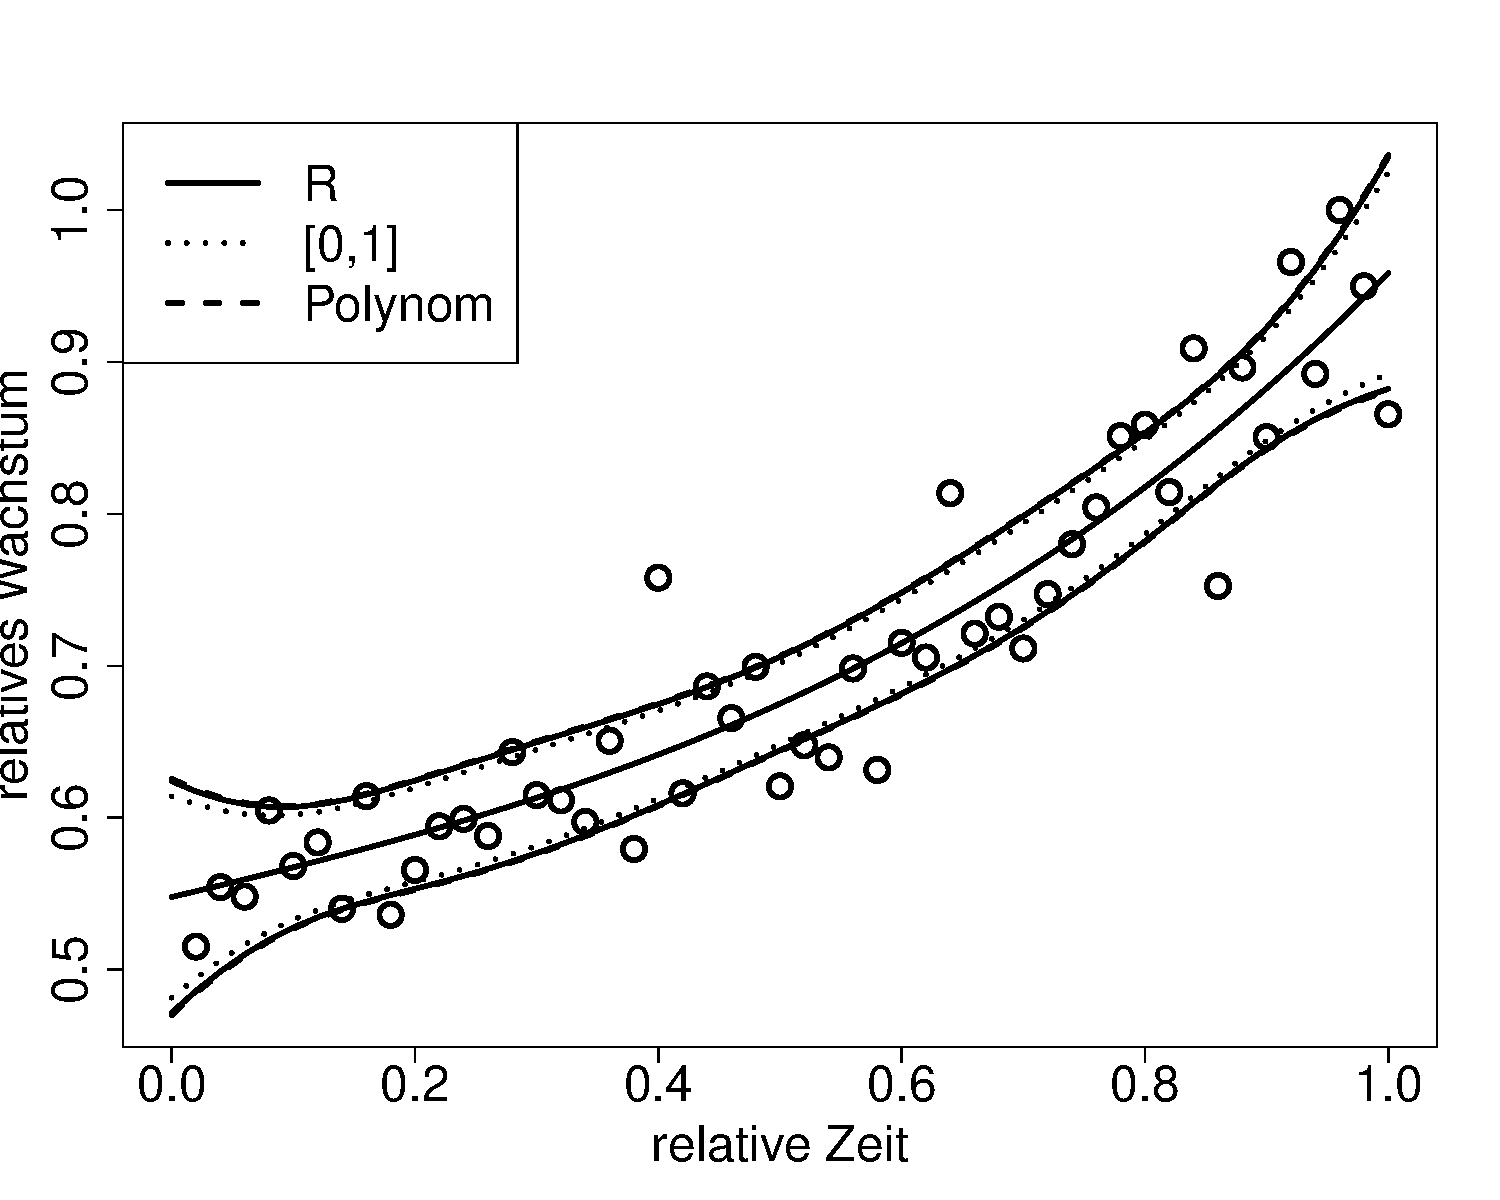
\includegraphics[width=0.5\textwidth]{Bsp-KB-poly}
  \caption{Daten aus Kapitel \ref{Regression und Konfidenzbaender} mit den drei Konfidenzbandarten}
  \label{KB-poly-BSP}
\end{figure}

Die kritischen Werte für das Konfidenzband auf ganz $\mathbb{R}^{3}$ und für das Konfidenzband auf [0,1] wurden in den vorherigen Abschnitten bereits berechnet. Es ergaben sich die Werte \cR ~und \cA . Berechnet man den kritischen Wert für das Konfidenzband auf [0,1], welches die Polynomgestalt berücksichtigt, erhält man den Wert \cAP . Dieser Wert ist noch kleiner als der Wert von \cA , was auch zu erwarten war.
\end{Beispiel}

\begin{Simulation}
Die Simulationstabelle aus den letzten beiden Abschnitt wird durch Überdeckungswahrscheinlichkeiten für die Konfidenzbänder auf einem Intervall $A$ beendet. In diesem Fall ist wieder $A = \{ (x_1, \ldots, x_p)' : 0 \leq x_i \leq 1, i=1, \ldots, p \}$ aufgrund der Struktur des Modells. Außerdem wird davon ausgegangen, dass die Designmatrix Polynomgestalt hat.

\begin{center}
\begin{tabular}{|c|c|c|c|}
\hline 
& unabhängig & AR bekannt & AR \\ 
\hline 
Konfidenzband auf ganz $\mathbb{R}^{p}$		 & \UeberRR		  & \UeberARbekanntR & \UeberARR \\ 
\hline 
Konfidenzband auf einem Polyeder	 & \UeberRMinmax  & \UeberARbekanntMinmax & \UeberARMinmax \\ 
\hline 
Konfidenzband auf einem Polyeder für Polynome  & \UeberRMinmaxPolyfast & \UeberARbekanntMinmaxPolyfast & \UeberARMinmaxPolyfast \\ 
\hline 
\end{tabular} 
\end{center}

\end{Simulation}





\newpage
\section{Vergleich von zwei Regressionsmodellen}
\label{Vergleich von zwei Regressionsmodellen}
Da das Ziel dieser Arbeit der Vergleich von Regressionsmodellen ist, wird in diesem Kapitel gezeigt, wie man Regressionsmodelle vergleicht. 

Es seien also, ähnlich wie in \cite[113]{Liu64} und \cite[178]{Liu64}, zwei Regressionsmodelle 

\begin{equation}
\label{Grundmodell_Hypothesentest}
Y_{i} = X_{i} \beta_{i} + e_{i} \text{ mit } i = 1,2  
\end{equation}

gegeben.

Dabei seien $Y_{i} = (Y_{i,1}, \ldots, Y_{i,n_i})$ für $i=1,2$ zwei Vektoren mit zufälligen Beobachtungen, die die abhängigen Daten darstellt.

Weiterhin seien $X_i$ für $i=1,2$ zwei $n_i \times (p+1)$ Designmatrix mit vollem Zeilenrang und festem Design. Dabei sei die $j$-te Zeile von $X_1$ mit der $j$-ten Zeile von $X_2$ für $j=1,\ldots, \min(n_1, n_2)$ identisch. Diese Bedingung bedeutet, dass beide Designmatrizen für $j=1, \ldots, \min(n_1, n_2)$ dasselbe, feste Design haben.

Außerdem seien $\beta_i$ zwei $(p+1) \times 1$ Koeffizientenvektoren, die den funktionalen Zusammenhang zwischen $Y_i$ und $X_i$ darstellen.

In diesem Kapitel sei $e_i \sim \mathscr{N}_{n_i}(0,\sigma^2 I_{n_i})$. Diese Annahme ist wichtig, da sich die Modelle somit nur in $\beta_i$ unterscheiden.

Die zugrunde liegenden Modelle sind also gleich, wenn $\beta_{1}=\beta_{2}$ 

Da die Werte von $\beta_{i}$ unbekannt sind und nur geschätzt werden können, testet man

\begin{equation}
H_{0} : \beta_{1} = \beta_{2}  \textbf{ vs. }  H_{1} : \beta_{1} \neq \beta_{2} \label{Hypothese}
\end{equation}

Dabei bezeichnet $H_{0}$ die \gls{Nullhypothese} und $H_{1}$ die Alternativhypothese.

Dazu ist es entweder möglich einen Test zu konstruieren oder Konfidenzbänder zu benutzen. In Abschnitt \ref{Vergleich F-Test} wird ein Test konstruiert und im Abschnitt \ref{Konfidenzbaender vergleich} werden Konfidenzbänder benutzt.

Es ist mit der in diesem Kapitel eingeführten Methode auch möglich zwei Modelle mit verschiedenen abhängigen Daten zu vergleichen. 

Ein Beispiel für solch ein Vorgehen ist der Vergleich des Blutdrucks von Männern und Frauen. Konkret kann man mit dieser Methode beispielsweise die Frage beantworten, ob sowohl für Männer als auch für Frauen der Zusammenhang zwischen Alter und Blutdruck gleich ist.

\begin{Beispiel}
Es wird das Beispiel aus Kapitel \ref{Regression und Konfidenzbaender} fortgeführt, indem eine zweite Designmatrix $X_2$ einführt wird. Die Designmatrix $X_2$ stellt ein polynomiales Modell vom Grad Vier dar. 

Das heißt, im Beispiel zu diesem Kapitel wird es darum gehen, ob es für die Daten, die bereits in Kapitel \ref{Regression und Konfidenzbaender} vorgestellt wurden, einen Unterschied macht, ein polynomiales Modell vom Grad Drei oder vom Grad Vier zugrunde zu legen. 

In der Abbildung \ref{Vergleich-Bsp} sind die beiden Modelle mit den Daten eingezeichnet.

\begin{figure}[H] 
  \centering
     \includegraphics[width=0.5\textwidth]{Bsp-beide-in-einem-plot}
  \caption{polynomielle Regression von Grad Drei und Grad Vier im Vergleich}
  \label{Vergleich-Bsp}
\end{figure}

%Im Folgenden sind die beiden Modelle in Matrixschreibweise angegeben:
%
%\[
%Y = \Ydat = \Xonedat \times \betaonedat + \edat = X_{1} \beta_{1} + e_{1}
%\]
%\[
%Y = \Ydat = \Xtwodat \times \betatwodat + \edat = X_{2} \beta_{2} + e_{2}
%\]
\end{Beispiel}




\subsection{F-Test zum Vergleich von zwei Regressionsmodellen}
\label{Vergleich F-Test}
Dieser Abschnitt beruht auf \cite[9-15]{Liu64} ,\cite[114-115]{Liu64} und \cite{Draper98}.

Zuerst betrachten wir den Test, der prüft, ob der Regressionskoeffizient $\beta$ eine lineare Einschränkung $Z \beta = d$ erfüllt. Dabei ist $Z$ eine gegebene $r \times (p+1)$ Matrix mit vollem Zeilenrang $r$ mit $1 \leq r \leq p+1$ und $d$ ist ein vorgegebener Vektor in $\mathbb{R}^r$. Wir wollen  also testen, ob

\begin{equation}
H_{0} : Z \beta = d  \textbf{ vs. }  H_{a} : Z \beta \neq d \label{Einschränkung_Hypothese}
\end{equation}

Von Interesse ist also, ob der Parameter in einem gegebenen Regressionsmodell eine lineare Einschränkung erfüllt.

Dazu wird zuerst der OLS-Schätzer $\hat{\beta}_Z$ unter der Bedingung, dass $Z \beta = d$ gilt, benötigt. Das heißt, $\hat{\beta}_Z$ minimiert

\begin{align*}
L(\beta) = (Y-X\beta)'(Y-X\beta) = \Vert Y - X \beta \Vert^2
\end{align*}

über alle $\beta \in \mathbb{R}^{p+1}$, die die Bedingung $Z \beta = d$ erfüllen. Man kann $\hat{\beta}_Z$ mittels Lagrange-Multiplikatoren finden. 

Betrachtet wird dazu der nachfolgende Satz.

\begin{Satz}
Unter den oben genannten Bedingungen ist der OLS-Schätzer $\hat{\beta}_Z$ gegeben durch 

\begin{equation*}
\hat{\beta}_Z=(X'X)^{-1}(X'Y+Z'f)= \hat{\beta}+(X'X)^{-1}Z'f
\end{equation*}

mit $f=(Z(X'X)^{-1}Z')^{-1}(d-Z\hat{\beta})$
\end{Satz}

\begin{proof}
Siehe \cite[13]{Liu64}
\end{proof}

Im Folgenden werden zwei Sätze aus \cite{Liu64} angegeben, die wir zur Konstruktion des Test im weiteren Verlauf dieses Abschnittes benötigen.

\begin{Satz}
Unter den oben genannten Bedingungen gilt
\begin{enumerate}
\item $\Vert X \hat{\beta} - X\hat{\beta}_Z \Vert^2  \sim \sigma^2 \chi_r^2(\delta)$ mit nicht zentralem Parameter 

$\delta = \Vert X \beta - X \mathbb{E}(\hat{\beta}_Z) \Vert^2 / \sigma^2 = (\beta - \mathbb{E}(\hat{\beta}_Z))' X'X (\beta - \mathbb{E}(\hat{\beta}_Z)) / \sigma^2$
\item $\Vert Y - X \hat{\beta}_Z \Vert^2  \sim \sigma^2 \chi_{n-(p+1)+r}^2(\delta)$ mit $\delta$ wie in 1.
\item $\Vert X \hat{\beta} - X\hat{\beta}_Z \Vert^2$ und $\Vert Y - X \hat{\beta}_Z \Vert^2$ sind unabhängig.
\item Außerdem ist
\begin{equation*}
\frac{\Vert X \hat{\beta}_Z - X\hat{\beta} \Vert^2 / r}{\Vert Y - X \hat{\beta} \Vert^2 / (n-p-1)} \sim f_{p+1,n-p-1}
\end{equation*}
\end{enumerate}
\end{Satz}

\begin{proof}
\cite[11]{Liu64}
\end{proof}

Damit kann ein Test zum Niveau $1-\alpha$ konstruiert werden:

\begin{equation}
\textnormal{Es ist }  H_0 \textnormal{ genau dann abzulehnen, wenn } \frac{\Vert X \hat{\beta}_Z - X\hat{\beta} \Vert^2 / r}{\Vert Y - X \hat{\beta} \Vert^2 / (n-p-1)} > f_{p+1,n-p-1}^{\alpha} \label{Einschränkung_Test}
\end{equation}

Dabei ist $f_{p+1,n-p-1}^{\alpha}$ das $\alpha-$Quantil der F-Verteilung mit den Freiheitsgraden $p+1$ und $n-p-1$.

Gleich wird noch folgender Satz aus \cite[13]{Liu64} benötigt:

\begin{Satz}
Es gilt 

\begin{equation*}
\Vert X \hat{\beta} - X \hat{\beta}_Z \Vert^2 = (Z \hat{\beta}-d)'(Z (X'X)^{-1} Z')^{-1} (Z \hat{\beta} - d)
\end{equation*}
\end{Satz}

\begin{proof}
\cite[13]{Liu64}
\end{proof}

Jetzt wird dieses Resultat auf den Vergleich von Regressionsmodellen angewendet. Dabei wird sich an \cite[114]{Liu64} orientiert. 

Betrachten wir wieder Modell \eqref{Grundmodell_Hypothesentest} vom Anfang dieses Kapitels. Außerdem wird wieder das Testproblem \eqref{Hypothese} betrachtet:

\begin{equation*}
H_{0} : \beta_{1} = \beta_{2}  \textbf{ vs. }  H_{1} : \beta_{1} \neq \beta_{2}
\end{equation*}

Um einen solchen Test durchzuführen, benötigt man eine Dummyvariable $z$:

\begin{equation*}
z=\begin{cases}
1 & \text{falls Y aus Modell 1 ist.}\\
0 & \text{falls Y aus Modell 2 ist.} 
\end{cases}
\end{equation*}

Mit $z$ können die beiden Modelle zu einem vereint werden, indem

\begin{equation}
Y = x' c_1 + z x' c_2 + e \label{Grundmodell_umformuliert}
\end{equation}
%= (x',z x') ???(c_1, c_2)??? + e

mit $x=(1,x_1,\ldots,x_p)'$, $c_1=\beta_2$ und $c_2=\beta_1-\beta_2$ gesetzt wird. Dass dieses Modell mit den beiden Modellen aus \eqref{Grundmodell_Hypothesentest} übereinstimmt, sieht man daran, dass

\begin{equation*}
Y = x'(c_1+c_2)+e = x'\beta_1+e
\end{equation*}

wenn $Y$ aus dem ersten Modell und 

\begin{equation*}
Y = x'c_1+e = x'\beta_2+e
\end{equation*}

wenn $Y$ aus dem zweiten Modell stammt. Damit kann man den Hypothesentest \eqref{Hypothese} umformulieren zu

\begin{equation*}
H_{0} : c_2 = \beta_1-\beta_2 = 0  \textbf{ vs. }  H_{1} : c_2 \neq 0 
\end{equation*}

Unter $H_{0}$ reduziert sich also das Gesamtmodell \eqref{Grundmodell_umformuliert} zu 

\begin{equation*}
Y = x' c_1 + e
\end{equation*}

Jetzt kann \eqref{Einschränkung_Test} benutzt werden und man erhält als Teststatistik : 

\begin{equation}
\textnormal{Es ist } H_0 \textnormal{ genau dann zu verwerfen, wenn } 
\frac{(\hat{\beta_1}-\hat{\beta_2})'D (\hat{\beta_1}-\hat{\beta_2})/(p+1)}{\widehat{\sigma^2}} > f^{\alpha}_{p+1,n-p-1}\label{Teststat_final}
\end{equation}

Dabei ist $\widehat{\sigma^2}$ die mittlere Varianz des Modells \eqref{Grundmodell_umformuliert}, $\hat{\beta_i} = (X_i'X_i)^{-1}X_iY$ und außerdem bezeichnet \gls{D}=$(X_1'X_1)^{-1}+(X_2'X_2)^{-1}$. 

Um zu sehen, dass \eqref{Teststat_final} tatsächlich aus \eqref{Einschränkung_Test} hergeleitet werden kann, ist folgende Rechnung nach \cite[115]{Liu64} zu betrachten. Dabei erfolgt in der Betrachtung allerdings ausschließlich die Berechnung für den Nenner.

%Für den Zähler betrachte:
%
%\begin{eqnarray*}
%X'X = \begin{bmatrix} X'_1 X_1 + X'_2 X_2 & X_1 X_1 \\ X'_1 X_1 & X'_1 X_1  \end{bmatrix} \\
%(X'X)^{-1} = \begin{bmatrix} (X'_2 X_2)^{-1} & -(X_2 X_2)^{-1} \\ -(X'_2 X_2)^{-1} & (X'_1 X_1)^{-1} + (X'_2 X_2)^{-1} \end{bmatrix} \\
%\hat{c} = \\
%\Vert Y - X \hat{c} \Vert^2 =
%\end{eqnarray*}
%
%Beachte, dass in diesem Fall die Matrix $A$ aus dem Test \eqref{Einschränkung_Hypothese} durch die $(p+1) \times 2(p+1)$ Matrix $(0,I_{p+1})$ und der Vektor $b$ durch den Nullvektor gegeben ist. Also ist der Zähler in \eqref{Einschränkung_Test} gegeben durch
%
%\[
%(A\hat{c}-b)'(A(X'X)^{-1}A')^{-1}(A\hat{c}-b)/r = (\hat{\beta}_1 - \hat{\beta}_2)' D (\hat{\beta}_1-\hat{\beta}_2)/(p+1)
%\]

Den Nenner der linken Seite von \eqref{Teststat_final} kann man schreiben als

\begin{align*}
\widehat{\sigma^2}  &= \frac{\Vert Y-X \hat{c} \Vert}{n_1 + n_2 - 2(p+1)} \\
				&= \frac{\Vert Y_1 - X_1 \hat{\beta_1} \Vert^2 + \Vert Y_2 - X_2 \hat{\beta_2} \Vert^2}{n_1+n_2-2(p+1)} \\
				&= \frac{n_1-p-1}{n_1+n_2-2(p+1)} \frac{\Vert Y_1 - X_1 \hat{\beta_1} \Vert^2}{n_1-p-1}+ \frac{n_2-p-1}{n_1+n_2-2(p+1)} \frac{\Vert Y_2 - X_2 \hat{\beta_2} \Vert^2}{n_2-p-1} \\
				&= \frac{n_1-p-1}{n_1+n_2-2(p+1)} \widehat{\sigma_{1}^2}+ \frac{n_2-p-1}{n_1+n_2-2(p+1)} \widehat{\sigma_{2}^2}
\end{align*}

Es wird nun das Beispiel aus der Einleitung zu diesem Kapitel fortgeführt.

\begin{Beispiel}
Berechnet man die Teststatistik \eqref{Teststat_final} erhält man als Teststatistik den Wert \TestWert ~und als kritischen Wert \kritWert . Also \EntscheidungHypothesen ~man die Hypothese. Die Modelle sind also \Modellesind .
\end{Beispiel}

Allerdings macht solch ein Test keinerlei Aussage über die Größe des Unterschiedes zwischen den Modellen. Deshalb werden im nächsten Abschnitt die Ergebnisse aus Kapitel \ref{Regression und Konfidenzbaender} benutzt.


\subsection{Vergleich von Regressionsmodellen mit Konfidenzbändern}
\label{Konfidenzbaender vergleich}
Dieser Abschnitt basiert auf \cite[119-121]{Liu64}.
Die grundlegende Idee ist, die Modelle voneinander abzuziehen und dann zu sehen, ob die Nullfunktion in einem Konfidenzband um die Differenz der beiden Modelle liegt.

Es wird dies nach \cite[122]{Liu64} formalisiert: 

Ein zweiseitiges, hyperbolisches, gleichmäßiges Konfidenzband für $x'\beta_2 - x'\beta_1$ über der Region $A$ hat die Form

\begin{equation} \label{Vergleich-KB}
x'\beta_2-x'\beta_1 \in x' \hat{\beta}_1 - x' \hat{\beta}_2 \pm c ~ \hat{\sigma} \sqrt{x' D x} ~ \text{ für alle } x \in A = (a,b)
\end{equation}

wobei $c$ eine kritische Konstante ist, sodass das Konfidenzniveau des Konfidenzbandes $1-\alpha$ beträgt. Dabei ist $D = (X_1'X_1)^{-1} + (X_2'X_2)^{-1}$

Sei $P$ die eindeutig bestimmte Wurzel aus $D = (X_1'X_1)^{-1} + (X_2'X_2)^{-1}$ und definiere weiterhin $T=P^{-1}(\hat{\beta}_2 - \beta_2 - \hat{\beta}_1 + \beta_1)/\hat{\sigma}$, welches wieder die $\tau_{p+1,v}$ Verteilung besitzt. Es folgt wie in Lemma \ref{Basiseigenschaft} , dass das simultane Konfidenzband \eqref{Vergleich-KB} gegeben ist durch $\mathbb{P}(S<c)$ mit

\begin{eqnarray*}
S &=& \sup_{x \in A} \frac{x' (\hat{\beta}_2-\beta_2-\hat{\beta}_1+\beta_1)}{\hat{\sigma}\sqrt{x' D x}}\\
&=& \sup_{x \in A} \frac{(Px)' (P^{-1} (\hat{\beta}_2-\beta_2-\hat{\beta}_1+\beta_1)/\hat{\sigma}}{\sqrt{(Px)'(Px)}} \\
&=& \sup_{x \in A} \frac{\vert (Px)' T \vert}{\Vert Px \Vert}
\end{eqnarray*}

Also kann die kritische Konstante $c$ genauso wie in Kapitel \ref{Konfidenzbaender auf einem Intervall fuer ein multiples lineares Regressionsmodell} beziehungsweise wie in Kapitel \ref{Konfidenzbaenderauf auf einem Intervall für Regressionsmodell mit Polynomgestalt} gefunden werden.

Jetzt zeigen wir noch ein Resultat, das zeigt, dass es keinen Unterschied macht, ob ein Test durchgeführt oder ein Konfidenzband auf ganz $\mathbb{R}^{p}$ benutzt wird. 

Betrachten wir den Test 

\begin{equation*}
H_0 : \beta = \beta_0 \textbf{ vs. } H_1 : \beta \neq \beta_0
\end{equation*}

Das heißt, es wird getestet, ob das Regressionsmodell $x' \beta$ dem wahren Modell $x' \beta_0$ entspricht. Dieser Test entspricht einem F-Test mit $Z=I_{p+1}$ und $\beta_0 = d$. Die Teststatistik ist nach \cite[17]{Liu64}

\begin{equation}\label{Test-Satz}
\textnormal{Es ist } H_0 \textnormal{ genau dann zu verwerfen, wenn } 
\frac{(\beta_0-\hat{\beta})' (X'X)^{-1} (\beta_0-\hat{\beta})}{(p+1) \Vert Y - X \hat{\beta} \Vert^2 / (n-p-1)} > f^{\alpha}_{p+1,n-p-1}\
\end{equation}

Satz und Beweis orientieren sich an \cite[67]{Liu64}.

\begin{Satz}
Der Test \eqref{Test-Satz} und Konfidenzbandmethode \ref{KB_Eigenschaft} akzeptieren und widerlegen $H_0$ immer dann, wenn auch die andere Methode akzeptiert beziehungsweise widerlegt.
\end{Satz}

\begin{proof}
Benutzt man die Definition von $N$ wie bisher, außer dass man $\beta$ mit $\beta_0$ ersetzt, erhält man

\begin{eqnarray*}
\sqrt{(p+1) f^{\alpha}_{p+1,n-p-1}} &<& \sup_{x_{(0)} \in \mathbb{R}^p} \frac{|x'(\hat{\beta}-\beta_0) |}{\hat{\sigma} \sqrt{x'(X'X)^{-1}x}} \\
&=& \sup_{x_{(0)} \in \mathbb{R}^p} \frac{| (Px)' N |}{(\hat{\sigma}/\sigma) \sqrt{(Px)'(Px)}} \\
&=& \frac{\Vert N \Vert}{(\hat{\sigma}/\sigma)} \Big( \sup_{x_{(0)} \in \mathbb{R}^p} \frac{| (Px)' N |}{\Vert P x \Vert \Vert N \Vert} \Big) \\
&=& \frac{\Vert N \Vert}{(\hat{\sigma}/\sigma)} \\
&=& \sqrt{ \frac{(\hat{\beta}-\beta_0)' P^{-1} P^{-1} (\hat{\beta}-\beta_0)}{\widehat{\sigma^2}} } \\
&=& \sqrt{\frac{(\hat{\beta}-\beta_0)' (X'X)^{-1} (\hat{\beta}-\beta_0)}{\widehat{\sigma^2}}}
\end{eqnarray*}

Dies entspricht der Teststatistik \eqref{Test-Satz}, also sind die beiden Tests äquivalent.
\end{proof}

Man beachte, dass in diesem Satz das Konfidenzband auf ganz $\mathbb{R}^{p}$ benutzt wurde. 

Das bedeutet, dass man mehr Informationen über ein gegebenes Entscheidungsproblem erhält, wenn man ein Konfidenzband berechnet, als wenn man einen Test durchführt. Dies liegt daran, dass das Konfidenzband auch eine Aussage über die Größe des Unterschiedes zwischen den Modellen macht.

Weiterhin wurde bereits im ersten Kapitel gezeigt, dass Konfidenzbänder auf einem Intervall und erst recht Konfidenzbänder für Polynome auf einem Intervall schmaler als Konfidenzbänder auf ganz $\mathbb{R}^{p}$ sind. Also ist es auch in dieser Hinsicht von Vorteil, Konfidenzbänder auf Intervallen zu verwenden.

%Was passiert, wenn eines der Modelle weniger Dimensionen (im Sinne der Designmatrix) als das andere hat ?

\begin{Beispiel}
Es wird jetzt das Beispiel aus dem Abschnitt \ref{Vergleich F-Test} fortgeführt, indem die Differenz der Regressionsmodelle geplottet wird und ein Konfidenzbänder auf $A$ für Polynome einfügt wird. Siehe dazu Abbildung \ref{KB-poly-hetero-BSP}.

\begin{figure}[H] 
  \centering
     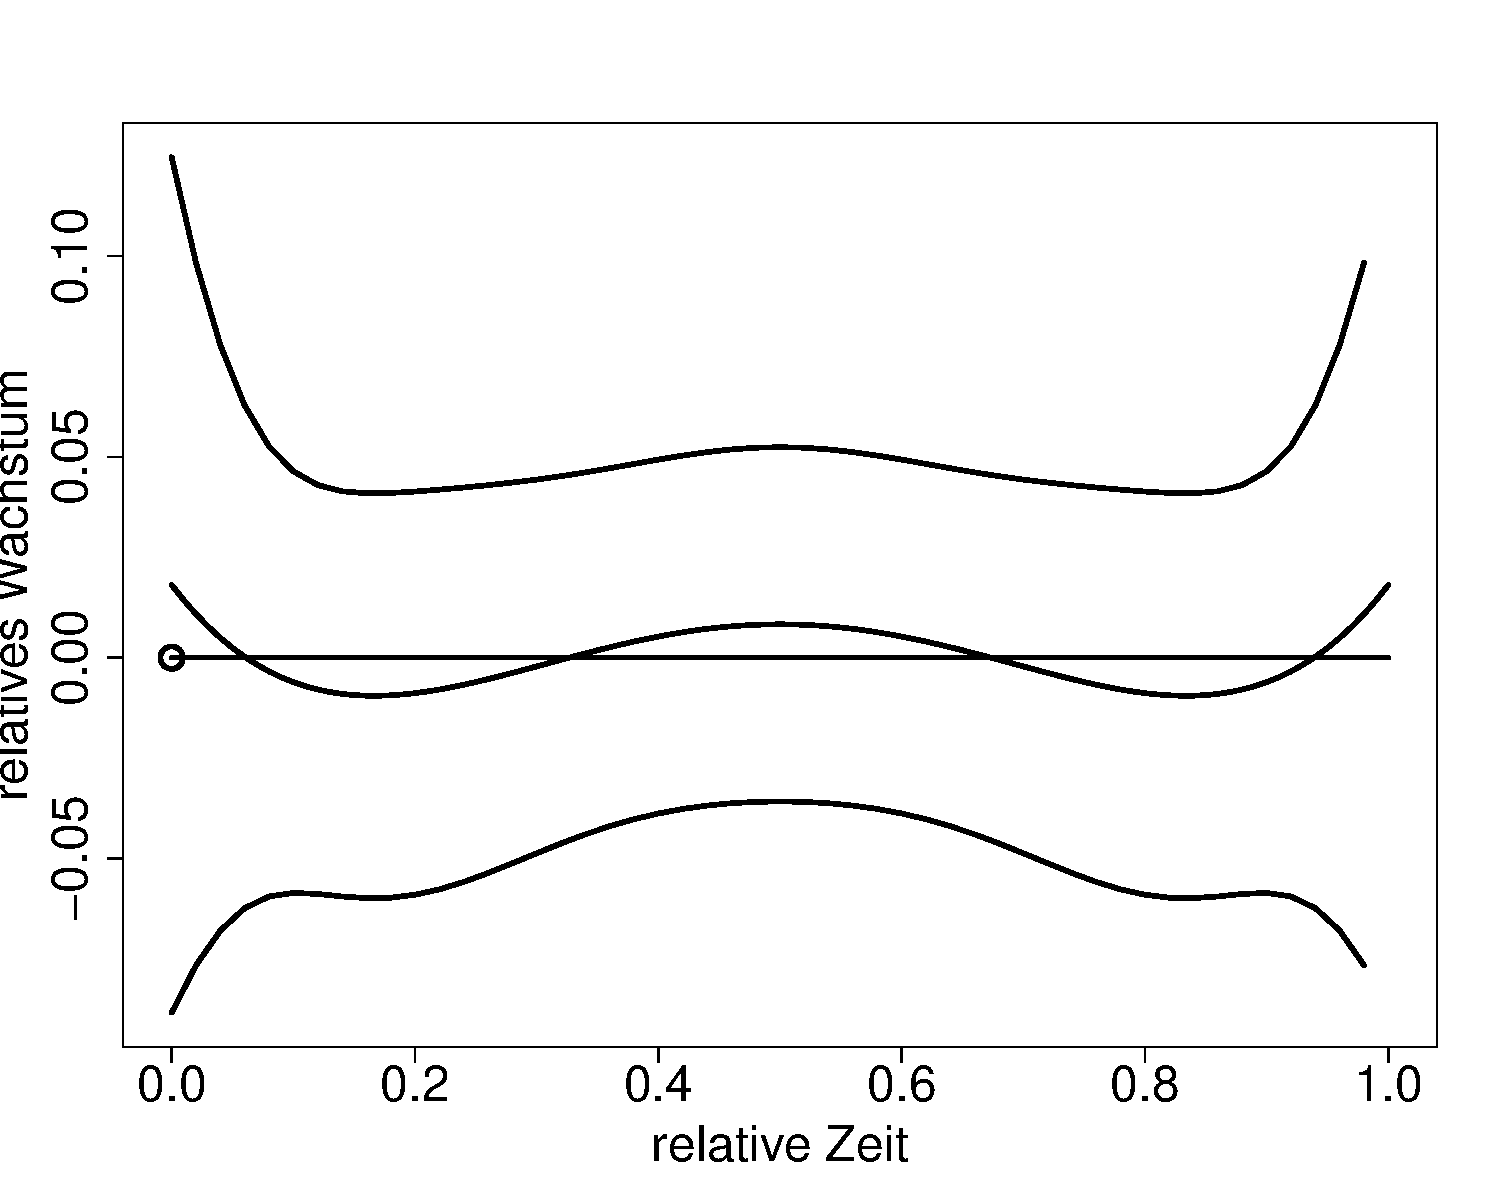
\includegraphics[width=0.5\textwidth]{Bsp-KB-poly-hetero}
  \caption{Differenz des Beispiels mit Konfidenzband auf A für Polynome}
  \label{KB-poly-hetero-BSP}
\end{figure}

Man sieht, dass die konstante Nullfunktion ganz im Konfidenzband enthalten ist. Also wird in diesem Fall die Nullhypothese nicht verworfen. Dies kann daran liegen, dass in diesem Test nur auf dem Intervall [0,1] getestet wird. Außerdem respektiert dieser Test die besondere Polynomstruktur des zugrunde liegenden Modells.

\end{Beispiel}


%\subsection{Konfidenzbänder auf einem Intervall}
%\label{Vergleich Konfidenzbaender auf einem Intervall}
%Dieser Abschnitt orientiert sich an \cite[121-123]{Liu64} und \cite{Jamshidian07} und \cite{Liu07}.
%
%
%\subsection{Konfidenzbänder auf einem Intervall, wenn das Regressionsmodell Polynomgestalt hat}
%\label{Vergleich Konfidenzbaender auf einem Intervall, wenn das Regressionsmodell Polynomgestalt hat}
%Dieser Abschnitt orientiert sich an \cite[197-200]{Liu64}.


\newpage
\section{Einen Teil eines Regressionsmodells überprüfen}
\label{Teil eines Regressionsmodells überprüfen}
In diesem Abschnitt geht es um den Spezialfall, zu prüfen, ob ein Teil des Regressionsmodells signifikant von Null verschieden ist oder nicht.  Das heißt, wir gehen von dem Modell

\begin{equation} \label{RegprüfModell}
Y=X \beta + e
\end{equation}

aus und wollen prüfen, ob einige der Koeffizienten $\beta_i$ gleich Null sind oder nicht. Ist $\beta_i$ gleich Null haben die zugehörigen unabhängigen Variablen $x_i$ keinen Einfluss auf die abhängige Variable $Y$.  

Zu diesem Zweck unterteilen wir den Vektor $\beta=(\beta_1,\beta_2)$ mit $\beta_1=(\beta_0, \ldots, \beta_{p-k})$ und $\beta_2=(\beta_{p-1+1}, \ldots, \beta_{p})$ für $1 \leq k \leq p$ eine gegebene natürliche Zahl. 

Auf die gleiche Art und Weise kann man die Spalten $x$ von $X$ in $x_1=(1,x_1, \ldots, x_{p-k})$ und $x_2=(1,x_{p-k+1}, \ldots, x_{p})$ unterteilen. Dabei wird das selbe $k$ für $\beta$ und für $X$ verwendet.

Ist $\beta_2=0$ so haben die unabhängigen Variablen $x_{p-k+1}, \ldots, x_p$ keinen Einfluss auf $Y$ und man kann Modell \eqref{RegprüfModell} zu 

\begin{equation}
Y=X_1 \beta_1 + e
\end{equation}

vereinfachen. Dabei ist $X_1$ die Matrix, die von den ersten $p-k+1$ Spalten von $X$ geformt wird.

\subsection{F-Test zum Überprüfen eines Teils eines Regressionsmodells}
\label{F-Test-Teil}
In diesem Abschnitt wird der F-Test als Methode, um zu überprüfen, ob $\beta_2=0$ ist, vorgestellt. Dieser Abschnitt orientiert sich an \cite[100-102]{Liu64}.

Ein Ansatz, um zu überprüfen, ob $\beta_2=0$ ist, ist der Test 

\begin{equation} \label{Test_prüfen}
H_{0} : \beta_{2} = 0  \textbf{ vs. }  H_{1} : \beta_{2} \neq 0
\end{equation}

der auch in \cite{Draper98} vorgeschlagen wird. Analog zu Abschnitt \ref{Vergleich F-Test} erhält man die Teststatistik

\begin{equation*}
\frac{(\tilde{I}\hat{\beta})'(\tilde{I}(X'X)^{-1}\tilde{I}')^{-1}(\tilde{I}\hat{\beta})/k}{\text{mean square residual von Modell \eqref{RegprüfModell}}} > f^{\alpha}_{k,v}
\end{equation*}

mit $v=n-p-1$, $\tilde{I}$ der $k \times (p+1)$ Matrix die durch $\tilde{I}=(0,I_k)$ gegeben ist und $f^{\alpha}_{k,v}$ dem $\alpha$ Quantil der $f$ Verteilung mit $k$ und $v$ Freiheitsgraden.

Dabei ist das mean squared residual von Modell \eqref{RegprüfModell} gegeben durch

\begin{equation*}
\text{MS} = \Vert Y - X\hat{\beta} \Vert^2 / (n-p-1) = \hat{\sigma}
\end{equation*}

Lehnt man bei diesem Test die Nullhypothese ab, heißt dies, dass es nicht genug statistisch gesicherte Hinweise gibt, um anzunehmen, dass $\beta_{2} = 0$ ist. Das heißt allerdings nicht, dass wir davon ausgehen können, dass $\beta_2 \neq 0$ ist. 

Benutzt man stattdessen ein Konfidenzband hat man ein Maß für den Unterschied der Modelle und kann eher entscheiden, ob $\beta_2 \neq 0$. Der nächste Satz macht genau solch eine Aussage.

\begin{Satz}
Es gilt
\begin{equation} \label{KB_R_prüfen}
\mathbb{P} \left( x_2'\beta_2 \in x_2'\hat{\beta_2} \pm \sqrt{k f^{\alpha}_{k,n-p-1}} \hat{\sigma} \sqrt{x_2' V x_2} \right) = 1 - \alpha
\end{equation}
\end{Satz}

Dabei ist $V=\tilde{I}(X'X)^{-1}\tilde{I}'$, $\hat{\beta_2} = \tilde{I} \hat{\beta}$ mit $\tilde{I}$ wie oben. 

Dieser Satz kann ähnlich wie Satz \ref{KB_Eigenschaft} bewiesen werden. Außerdem gilt folgender Satz.

\begin{Satz}
Test \eqref{Test_prüfen} und das Konfidenzband \eqref{KB_R_prüfen} verwerfen und akzeptieren $H_0$ zur selben Zeit.
\end{Satz}

Das Konfidenzband \eqref{KB_R_prüfen} gibt einem also immer mehr Informationen. Allerdings ist das Konfidenzband auf ganz $R^k$ definiert. Eine noch besser Aussage über $H_0$ kann man also treffen, wenn man stattdessen ein Konfidenzband auf $A$ betrachtet. 

\subsection{Einen Teil eines Regressionsmodells auf einem Intervall überprüfen}
\label{Teil eines Regressionsmodells auf einem Intervall überpruefen}
Dieser Abschnitt orientiert sich an \cite[102-105]{Liu64}.

Wir beschränken uns auf die rechteckige Region

\begin{equation*}
A_2 = \{ x_2 \in \mathbb{R}^k =(x_{2,p-k+1}, \ldots x_{2,p}) : x_{2,1} \in [a_i,b_i], i=p-k+1, \ldots, p \}
\end{equation*}

Dabei sind $- \infty \leq a_i \leq b_i \leq \infty, i = p-k+1, \ldots, p$ gegebene Konstanten. Ein hyperbolisches Konfidenzband auf $A_2$ ist gegeben durch

\begin{equation}\label{KB_pruefen}
x_2'\beta_2 \in x_2'\hat{\beta_2} \pm c \hat{\sigma}\sqrt{x_2'Vx_2} \text{ für alle } x_2 \in A_2
\end{equation}

dabei muss man die kritische Konstante $c$ so bestimmen, dass das gleichmäßige Konfidenzniveau $1 - \alpha$ ist.

Sei $W$ die Wurzel aus $V$, also sei $V=W^2$. Bezeichne $N_2=W^{-1}(\hat{\beta_2}-\beta_2)/\sigma \sim \mathscr{N}_{k}(0,I)$ und $T_2 = N_2/(\hat{\sigma}/\sigma \sim \tau_{k,v}$. Dann ist das Konfidenzlevel von \eqref{KB_pruefen} gegeben durch $\mathbb{P}(S<c)$ wobei

\begin{eqnarray*}
S &=& \sup_{x_2 \in A_2} \frac{\vert x_2' (\hat{\beta_2} - \beta_2) \vert }{\hat{\sigma} \sqrt{x_2' V  x_2}} \\
&=& \sup_{x_2 \in A_2} \frac{\vert (Wx_2)'W^{-1} (\hat{\beta_2}-\beta_2)/\hat{\sigma} \vert}{\sqrt{(Wx_2)'(Wx_2)}} \\
&=& \sup_{v \in C(W,A_2)} \frac{\vert v'T_2 \vert }{\Vert v \Vert}
\end{eqnarray*}

Dabei gilt $C(W,A_2)=\{ \lambda W x_2 = \lambda(x_{p-k+1} w_1 + \ldots + x_p w_k) : \lambda > 0 \text{ and } x_2 \in A_2 \}$ mit $W=(w_1, \ldots, w_k)$. 

Die Verteilung von $S$ hängt nicht von $\beta$ und $\sigma$ ab. Allerdings hängt sie in komplizierter Weise von der Region $A_2$ und $W$ durch $C(W,A_2)$ ab.

Für die beiden Spezialfälle $k=1$ und $0 \in C(W,A_2)$ ergeben sich Vereinfachungen. Im allgemeinen Fall kann man $c$ ähnlich wie in Abschnitt \ref{Konfidenzbaender auf einem Intervall fuer ein multiples lineares Regressionsmodell} finden. Dazu berechnet man $R$ mal $S_i$ auf die folgende Art:

\begin{enumerate}
\item Simuliere $N_2 \sim \mathscr{N}_{k}(0,I)$ und $\hat{\sigma}/\sigma \sim \sqrt{\chi^2_v/v}$
\item Bestimme $\Vert \pi^{*}(T_2,W,A_2) \Vert$ und $\Vert \pi^{*}(-T_2,W,A_2) \Vert$
\item Dann ist $S= \max(\Vert \pi^{*}(T_2,W,A_2) \Vert, \Vert \pi^{*}(-T_2,W,A_2) \Vert )$
\end{enumerate}

Dann ist die kritische Konstante $c$ das $1-\alpha$ Quantil von $S_1, \ldots, S_R$.

Die Berechnung von $\Vert \pi^{*}(T_2,W,A_2) \Vert$ findet man in \cite[Appendix B]{Liu64}.

Diese Methode wurde nicht weiter verfolgt, da das Ziel dieser Arbeit ist, Konfidenzbänder zu vergleichen. Außerdem werden im Kapitel \ref{Datenbeschreibung und Resultate} vor allem Polynommodelle betrachtet. Wie man in diesem Fall Konfidenzbänder konstruiert ist Thema des nächsten Abschnitts.

\begin{Simulation}
Es werden für das Konfidenzband auf ganz $\mathbb{R}^{p}$ wieder eine Simulation für die Überdeckungswahrscheinlichkeit für Daten aus einer gewöhnlichen multilinearen Regression und einer Regression mit AR(1)-Kovarianzmatrix durchgeführt:


\begin{center}
\begin{tabular}{|c|c|c|c|}
\hline 
 & unabhängig & AR bekannt & AR \\ 
\hline 
Konfidenzband auf ganz $\mathbb{R}^{p}$		 & \UeberRR		  & \UeberARbekanntR & \UeberARR \\ 
\hline 
Konfidenzband auf einem Polyeder	 & \UeberRMinmax  & \UeberARbekanntMinmax & \UeberARMinmax \\ 
\hline 
Konfidenzband auf einem Polyeder für Polynome  & \UeberRMinmaxPolyfast & \UeberARbekanntMinmaxPolyfast & \UeberARMinmaxPolyfast \\ 
\hline 
 Teil des Modells auf $\mathbb{R}^{p}$ überprüfen 	& \UeberRRpruefen & - & \UeberARRpruefen \\ 
\hline 
\end{tabular} 
\end{center}

\end{Simulation}



\subsection{Einen Teil eines Regressionsmodells überprüfen, wenn das Modell Polynomgestalt hat}
\label{Teil eines Regressionsmodells überpruefen, wenn das Modell Polynomgestalt hat}
Dieser Abschnitt orientiert sich an \cite[190-192]{Liu64} und \cite{Draper98}.

Für den Fall, dass man Modelle mit Polynomgestalt betrachtet erhält man als F-Test

\begin{equation}\label{KB hypo prüfen}
\text{lehne } H_0 \text{ ab } \Leftrightarrow \frac{\hat{\beta_2}' V^{-1} \hat{\beta_2}/k}{\widehat{\sigma^2} }> f^{\alpha}_{k,v}
\end{equation}

Dabei ist $\hat{\beta_2}$ der Schätzer für $\beta_2=(b_{p-k+1}, \ldots b_{p})'$ welcher die letzten $k$ Komponenten von $\beta$ ist. Dieser Schätzer hat Verteilung $\mathscr{N}(\beta_2,\sigma^2,V)$. Außerdem ist $V$ die $k \times k$ Matrix, die von den letzten $k$ Zeilen und den letzten $k$ Spalten von $(X'X)^{-1}$ erzeugt wird. Da $V$ nicht singulär ist, sei $W$ die eindeutig bestimmte Wurzel von $V$, das heißt $V=W^2$. 

Analog zum letzten Abschnitt kann wieder gezeigt werden, dass dieser Test dem Konfidenzband 

\begin{equation}\label{KB poly prüfen}
x_2' \beta_2 \in x_2' \hat{\beta_2} \pm \sqrt{k f^{\alpha}_{k,v}} \hat{\sigma} \sqrt{x_2' V x_2} \text{ für alle } x_2 \in \mathbb{R}^k
\end{equation}

entspricht. Das heißt, liegt die Nullfunktion nicht vollständig im Konfidenzband \eqref{KB poly prüfen}, kann man die Nullhypothese aus Test \eqref{KB hypo prüfen} ablehnen.

Analog zu Abschnitt \ref{Konfidenzbaenderauf auf einem Intervall für Regressionsmodell mit Polynomgestalt} kann man wieder ein Konfidenzband auf einem Intervall $A$ konstruieren, das die Polynomstruktur berücksichtigt.

Dazu betrachtet man, dass das Konfidenzniveau von \eqref{KB poly prüfen} für $c$ anstatt $\sqrt{k f^{\alpha}_{k,v}}$ durch den Ausdruck $\mathbb{P}(S\leq c)$ gegeben ist. Dabei ist

\begin{eqnarray*}
S &=& \sup_{x \in A} \frac{\vert \tilde{x_2}' (\hat{\beta_2}-\beta_2)}{\hat{\sigma} \sqrt{\tilde{x_2'}V\tilde{x_2}}} \\
&=& \sup_{x \in A} \frac{\vert (1, \ldots, x^{k-1})(\hat{\beta_2}-\beta_2}{\hat{\sigma} \sqrt{(1, \ldots, x^{k-1}) V (1, \ldots x^{k-1})'}}
\end{eqnarray*}

mit $\tilde{x_2}= x^{p-k+1}(1, x, \ldots, x^{k-1})$.

Also ist die kritische Konstante $c$ genau so wie in Abschnitt \ref{Konfidenzbaenderauf auf einem Intervall für Regressionsmodell mit Polynomgestalt} berechenbar, außer dass man $p=k-1$ und $(X'X)^{-1}$ mit $V$ ersetzen muss. Die Simulation ändert sich allerdings nicht.

\begin{Simulation}
Auch für die Methode aus diesem Abschnitt wurden Simulationen durchgeführt:

\begin{center}
\begin{tabular}{|c|c|c|c|}
\hline 
& unabhängig & AR bekannt & AR \\ 
\hline 
Konfidenzband auf ganz $\mathbb{R}^{p}$		 & \UeberRR		  & \UeberARbekanntR & \UeberARR \\ 
\hline 
Konfidenzband auf einem Polyeder	 & \UeberRMinmax  & \UeberARbekanntMinmax & \UeberARMinmax \\ 
\hline 
Konfidenzband auf einem Polyeder für Polynome  & \UeberRMinmaxPolyfast & \UeberARbekanntMinmaxPolyfast & \UeberARMinmaxPolyfast \\ 
\hline 
Teil des Modells auf $\mathbb{R}^{p}$ überprüfen 	& \UeberRRpruefen & - & \UeberARRpruefen \\ 
\hline 
Teil des Modells auf A für Polynome überprüfen	& \UeberRMinmaxPolyfastpruefen & - & \UeberARMinmaxPolyfastpruefen \\ 
\hline 
\end{tabular} 
\end{center}

\end{Simulation}

%\subsection{Ausblick: Vergleich mit der Nullfunktion}
%\label{Ausblick: Vergleich mit der Nullfunktion}
%Dieser Abschnitt orientiert sich an \cite[110-112]{Liu64}.




\newpage
\section{Regression und Konfidenzbänder für abhängige Daten}
\label{Regression und Konfidenzbänder für abhaengige Daten}
Alle bisherigen Ergebnisse beruhen auf dem homoskedastischen, multiplen linearen Regressionsmodell. Das heißt, mit $Y=(y_1, \ldots, y_n) \in \mathbb{R}^n$, $\beta \in \mathbb{R}^{p+1}$ und $X \in \mathbb{R}^{n \times (p+1)}$ wurde von dem funktionalem Zusammenhang

\begin{align} \label{Grundmodell_AR}
Y = X \beta + e
\end{align}

ausgegangen, wobei $e \sim \mathscr{N}_{n}(0, \sigma^2 I_n)$ war.  Es wurden für dieses Modell Konfidenzbänder mit verschiedenen Designmatritzen $X$ sowohl auf $\mathbb{R}^{p}$ als auch auf einem Intervall $A$ bestimmt.

In diesem Kapitel wird der Fall betrachtet, dass die Fehler untereinander korreliert sind. 

Zuerst werden wir autoregressive Modelle und im besonderen Zeitreihen, die einem AR(1) Prozess folgen, eingeführt. Dieser erste Abschnitt orientiert sich an \cite{Hansen15} und \cite{Brockwell91}.

Danach betrachten wir die Berechnung von Schätzern für die Parameter von Zeitreihen. Dazu sollen Funktionen aus dem R Paket \textit{nlme}, dies steht für \textit{nonlinear mixed-effects models}, verwendet werden. Dazu wird die Quelle \cite{Pinheiro00} verwendet.

In Abschnitt \ref{Konfidenzbaender für AR(1)} dieses Kapitels werden Methoden angegeben, wie wir für abhängige Daten Konfidenzbänder konstruieren können. Das heißt, wir betrachten wie die beiden vorhergehenden Abschnitte die Überlegungen aus den Abschnitten \ref{Konfidenzbaenderauf auf einem Intervall für Regressionsmodell mit Polynomgestalt} und \ref{Teil eines Regressionsmodells überpruefen, wenn das Modell Polynomgestalt hat} ändern.


\subsection{Autoregressive Modelle und AR(1)}
\label{Regression für AR(1)}
In diesem Abschnitt wird Modell \eqref{Grundmodell_AR} auf den Fall von abhängigen Daten verallgemeinert. Daten sind abhängig, wenn $\text{Cov}(y_i,y_j) \neq 0$ für $i \neq j$.

Beginnen wir mit ein paar Definitionen. Die erste orientiert sich an \cite[1]{Brockwell91}.

\begin{Definition}
\textbf{Zeitreihe}

Eine Zeitreihe $X$ ist eine Menge von Messungen $x_t$ an bestimmten Zeitpunkten $t$. 

Bei einer diskreten Zeitreihe ist $ t=1, \ldots, T $ mit $T \in \mathbb{N}$ fest. 
\end{Definition}

Weiterhin brauchen wir die folgende Definition, die \cite{Hansen15} entnommen ist.

\begin{Definition}
\textbf{stationäre Zeitreihe}

Eine Zeitreihe $X = (X_t)$ nennt man stationär, wenn $\mathbb{E}(X_t) = \mu$ unabhängig von $t$ ist und Cov($X_t,X_{t-k})$) = $\gamma (k)$ unabhängig von $t$ für alle $k$ ist.
\end{Definition}

Eine besondere Zeitreihe ist ein so genannter \textit{autoregressive-moving average} (ARMA) Prozess. Die folgende Definition orientiert sich an \cite[78]{Brockwell91}.

\begin{Definition}
\textbf{ARMA(p,q) Prozess}

Den Prozess $(X_t)$ nennt man einen ARMA(p,q) Prozess, wenn $(X_t)$ stationär ist und für jedes $t$ gilt

\begin{equation}\label{ARMA}
X_t - \phi_1 X_{t-1} - \ldots - \phi_p X_{t-p} = Z_t + \theta_1 Z_{t-1} + \ldots + \theta_q Z_{t-q}
\end{equation}

mit $(Z_t) \sim \text{WN}(0, \sigma^2)$.  Dabei sagt man, dass der Prozess $(Z_t) \sim \text{WN}(0, \sigma^2)$ ist, wenn $(Z_t)$ Erwartungswert Null und eine Kovarianzfunktion der Form

\begin{equation*}
\gamma(h) = \begin{cases} \sigma^2 &, \text{ falls } h=0 \\ 0 &, \text{ falls } h \neq 0 \end{cases}
\end{equation*}
\end{Definition}

Die Gleichung \eqref{ARMA} kann man kompakter als

\begin{equation*}
\phi(B) X_t = \theta(B) Z_t, t \in 0, \pm 1, \pm 2, \ldots
\end{equation*}

schreiben. Dabei sind $\phi$ und $\theta$ die Polynome

\begin{equation*}
\phi(z) = 1 - \phi_1 z - \ldots - \phi_p z^p
\end{equation*}

und 

\begin{equation*}
\theta(z) = 1 + \theta_1 z + \ldots + \theta_q z^q
\end{equation*}

und $B$ ist der Rückwärtsshift-Operator definiert durch

\begin{equation*}
B^j X_t = X_{t-j},~~ j = 0, \pm 1, \pm 2, \ldots
\end{equation*}

Es gibt verschiedene Arten von ARMA Prozessen. Uns werden im folgenden nur so genannte autoregressive Prozesse erster Ordnung (AR(1)), ein Spezialfall von allgemeinen ARMA Prozessen, interessieren.

\begin{Definition}
\textbf{AR(p)}

Ist in der obigen Definition $\theta(x) \equiv 1$, so ist 

\begin{equation*}
\phi(B) X_t = Z_t
\end{equation*}

und man nennt den Prozess einen autoregressiven Prozess von Ordnung $p$ (oder AR(p)).
\end{Definition}

Ein Spezialfall von AR(p) Prozessen ist der AR(1) Prozess, bei dem gilt

\begin{align}
y_t = \phi y_{t-1} + e_t
\end{align}

Dabei ist \gls{phi} ein unbekannter Parameter und $\mathbb{E}(e_t)=0$, $\mathbb{E}(e_t^2)=\sigma^2 < \infty$. Für den Fall, dass $\phi \in (-1,1)$ ist, nennt man die Zeitreihe streng stationär und ergodisch. 

Da die Messungen nacheinander getätigt werden, steht zu vermuten, dass $y_t$ und $y_{t+1}$ auf irgendeine Art und Weise nahe beieinander sind. Ist dies der Fall, sind $y_t$ und $y_{t+1}$ nicht unabhängig. Unabhängigkeit war allerdings eine der zentrale Annahmen im ersten Kapitel. Deshalb muss man die Schätzer für die Parameter des Modells auf eine andere Art bestimmen.

Bei AR(1)-Prozessen hängt der Wert zur Zeit $t$ offenbar vom Wert der Zeitreihe zur Zeit $t-1$ ab. Somit ist hier $\text{Cov}(y_i,y_j) \neq 0$ für $i \neq j$ und die Ergebnisse aus Kapitel \ref{Regression und Konfidenzbaender} können nicht angewendet werden. 

Man kann $\text{Cov}(y_i,y_j)$ durch den funktionalen Zusammenhang $\mathbb{E}(Y_i) = \phi^{i-j} \mathbb{E}(Y_{j})$ für $i>j$ finden. Für $j<i$ ist $\mathbb{E}(Y_j) = \phi^{i-j} \mathbb{E}(Y_i)$. 

Beispielsweise erhält man für $i=1$ den Zusammenhang $y_1 = \phi^j y_j$ und somit

\begin{eqnarray*}
\text{Cov}(y_1, y_j) &=& \mathbb{E}((\mathbb{E}(y_1)-y_i)(\mathbb{E}(y_j)-y_j)) \\
&=& \mathbb{E}(\mathbb{E}(y_1)\mathbb{E}(y_j) - \mathbb{E}(y_1)y_j - \mathbb{E}(y_j)y_i +y_j y_1) \\
&=& \phi^j \mathbb{E}(\mathbb{E}(y_j^2) - 2 \mathbb{E}(y_j)y_j + y_j^2) \\
&=& \phi^j \mathbb{E}(\mathbb{E}(y_j^2)-\mathbb{E}(y_j)^2) \\
&=& \phi^j \sigma^2
\end{eqnarray*}

Damit hat die Korrelationsmatrix \gls{Xi} von $e$ in diesem Fall die Form

\begin{equation}\label{Upsilon}
\Upsilon = 
\left[
   \begin{array}{cccccc}
     1 				& \phi 			& \phi^2	& \cdots	& \phi^{n-2}	& \phi^{n-1} 	\\
     \phi 			& 1		 		& \phi 		& \cdots	& \phi^{n-3}	& \phi^{n-2} 	\\
     \phi^2 		& \phi 			& 1		 	& \ddots	& \vdots		& \vdots 		\\
     \vdots		 	& \vdots	 	& \ddots	& \ddots	& \phi			& \phi^{2} 	\\
     \phi^{n-2} 	& \phi^{n-3}	& \cdots 	& \phi		& 1				& \phi 		\\
     \phi^{n-1} 	& \phi^{n-2} 	& \cdots	& \phi^{2}	& \phi			& 1  
   \end{array}
\right]
\end{equation}

Das heißt, das Modell ist gegeben durch 

\begin{align} \label{AR Modell}
Y = X \beta + e
\end{align}

mit $e \sim \mathscr{N}_{n}(0,\Upsilon)$.



\subsection{AR(1) und das \textit{nlme} Paket}
\label{AR(1) und das nlme Paket}

In diesem Abschnitt wird vorgestellt, wie die Schätzer für $\beta$, $\sigma$ und $\phi$ konkret berechnet werden können. Dieser Abschnitt orientiert sich an \cite[203-205]{Pinheiro00}.

Um einen ML-Schätzer für Modell \eqref{AR Modell} zu erhalten, kann man folgenden Trick anwenden: Man multipliziert beide Seiten der Gleichung mit $\Upsilon^{-1/2}$. Dann wird aus Modell \eqref{AR Modell} wieder Modell \eqref{Grundmodell_AR}, wenn auch mit anderen Werten. Konkret erhält man

\begin{align} \label{AR rück}
(\Upsilon^{-1/2})Y = Y^{*} = X^{*} \beta + e^{*} = (\Upsilon^{-1/2})X + (\Upsilon^{-1/2})e
\end{align}

mit $e^{*} = (\Upsilon^{-1/2})e \sim \Upsilon^{-1/2} \cdot \mathscr{N}_{n}(0,\Upsilon) = \mathscr{N}_{n}(0,\Upsilon^{-1}\Upsilon) = \mathscr{N}_{n}(0,I)$. Die Schwierigkeit besteht also darin, die Konstante $\phi$ zu bestimmen. 

Die Konstante $\phi$ wird mittels \textit{profiled-maximum-liklihood}-Schätzung bestimmt. Dazu fixiert man zuerst $\phi$ und berechnet die ML-Schätzer für $\hat{\beta}$ und $\widehat{\sigma^2}$ mittels:

\begin{eqnarray}
\label{profile beta}
\hat{\beta}(\phi) =  \big( (X^*)' X^* \big)^{-1} (X^*)' Y^* \\
\widehat{\sigma^2}(\phi) = \frac{\Vert Y^* - X^* \hat{\beta}(\phi) \Vert^2}{n-p-1} \nonumber
\end{eqnarray}

Danach setzt man \eqref{profile beta} in die normale Likelihoodfunktion von Modell \eqref{AR rück} ein und erhält:

\begin{equation}\label{ML-phi}
l(\phi|Y) = \text{const} - (n-p-1) \log \Vert Y^* - X^* \hat{\beta}(\phi) \Vert - \frac{1}{2} \sum^n_{i=1} \log( \text{det} (\Upsilon) )
\end{equation}

Man findet dann $\hat{\phi}$ indem man das Argmax von \eqref{ML-phi} für $\phi$ bestimmt. Dies geschieht in dem Paket \textit{nlme} numerisch mittels orthogonal-triangulären Zerlegungen. Sieh hierzu \cite[68-75]{Pinheiro00}.

Um den Wert von $\hat{\phi}$ für vorgegebene Daten zu bestimmen, wurde die Funktion \textit{gls} aus dem Paket \textit{nlme} benutzt. Bei der Benutzung von \textit{gls}, um einen Schätzer für $\phi$ zu bestimmen, muss der Wert \textit{correlation=corAR1()} an \textit{gls} übergeben werden.

Um dann bei gegebenem $\phi$ beziehungsweise $\hat{\phi}$ einen Schätzer für $\beta$ und $\sigma$ zu bestimmen, wird folgender Algorithmus verwendet:

\begin{enumerate}
\item Benutze gls um $\phi$ zu bestimmen.
\item Bestimme $\Upsilon$ und mittels der R-Funktion \textit{solve} $\Upsilon^{-1}$ 
\item Führe eine Eigenwertzerlegung von $\Upsilon^{-1}$ durch, um die Matrix $\Upsilon^{-1}$ zu diagonalisieren und nehme dann von der Hauptdiagonalenmatrix elementenweise die Wurzel, um $\Upsilon^{-1/2}$ zu bestimmen.
\item Transformiere $Y$ nach $Y^{*}$ und $X$ nach $X^{*}$ mittels Linksmultiplikation mit $\Upsilon^{-1/2}$
\item Benutze eine normale OLS um $D=(X^{'*}X^{*})^{-1}$, $\beta$ und $\sigma^2$ zu berechnen.
\end{enumerate}

Führt man diese Schritte durch, das heißt man transformiert die Daten und berechnet dann den OLS Schätzer 

\begin{equation*}
\hat{\beta} = (X^{t} X)^{-1} X^{t} Y
\end{equation*}

für die transformierten Daten 

\begin{equation*}
\Upsilon^{-1/2} Y = \Upsilon^{-1/2} X \beta + \Upsilon^{-1/2} e
\end{equation*}

erhält man

\begin{eqnarray*}
\hat{\beta} &=& ((\Upsilon^{-1/2} X)^{t} \Upsilon^{-1/2} X)^{-1} (\Upsilon^{-1/2} X)^{t} \Upsilon^{-1/2} Y \\
&=& (X^{t} \Upsilon^{-1/2} \Upsilon^{-1/2})^{-1} X^{t} \Upsilon^{-1/2} \Upsilon^{-1/2} Y \\
&=& (X^{t} \Upsilon^{-1} X)^{-1} X^{t} \Upsilon^{-1} Y
\end{eqnarray*}
 
Was genau der \textit{generalised least squares} (GLS) Schätzer ist.

Dies entspricht dem Vorgehen der Funktion \textit{gls} aus dem \textit{nlme} Paket. Deswegen wird in Zukunft immer direkt der \textit{gls} Schätzer benutzt.

\begin{Beispiel}
Jetzt wird das Beispiel aus Abschnitt \ref{Regression} fortgeführt, indem eine Regression mit AR(1) für das Polynommodell mit Grad Drei durchgeführt wird. 

Die Daten werden wie im ersten Abschnitt dieser Arbeit erzeugt. Das heißt, es werden $\beta, \sigma$ und $X$ initialisiert. Dann wird $e$ simuliert. In diesem Beispiel gehe wir allerdings davon aus, dass $e \sim \mathscr{N}_n(0, \sigma^2 \Upsilon)$. Dabei ist die Korrelatiosmatrix $\Upsilon$ von der Form 

\[
\Upsilon = 
\left[
   \begin{array}{cccccc}
     1 				& \phi 			& \phi^2	& \cdots	& \phi^{n-2}	& \phi^{n-1} 	\\
     \phi 			& 1		 		& \phi 		& \cdots	& \phi^{n-3}	& \phi^{n-2} 	\\
     \phi^2 		& \phi 			& 1		 	& \ddots	& \vdots		& \vdots 		\\
     \vdots		 	& \vdots	 	& \ddots	& \ddots	& \phi			& \phi^{2} 	\\
     \phi^{n-2} 	& \phi^{n-3}	& \cdots 	& \phi		& 1				& \phi 		\\
     \phi^{n-1} 	& \phi^{n-2} 	& \cdots	& \phi^{2}	& \phi			& 1  
   \end{array}
\right]
\]

mit dem fest gewähltem Wert $\phi = \phitrue$.

Man erhält als Schätzer für den AR(1) Parameter $\hat{\phi}$ = \phiestone , während der wahre Wert \phitrue ~ist.

Als Schätzung für die Parameter erhält man \betaARone ~und \sigmaARone , während die wahren Werte \betatrue ~und \sigmatrue ~sind. 

Zeichnet man dann dieses Regressionspolynom mit den Daten in eine Abbildung erhält man

\begin{figure}[H] 
  \centering
     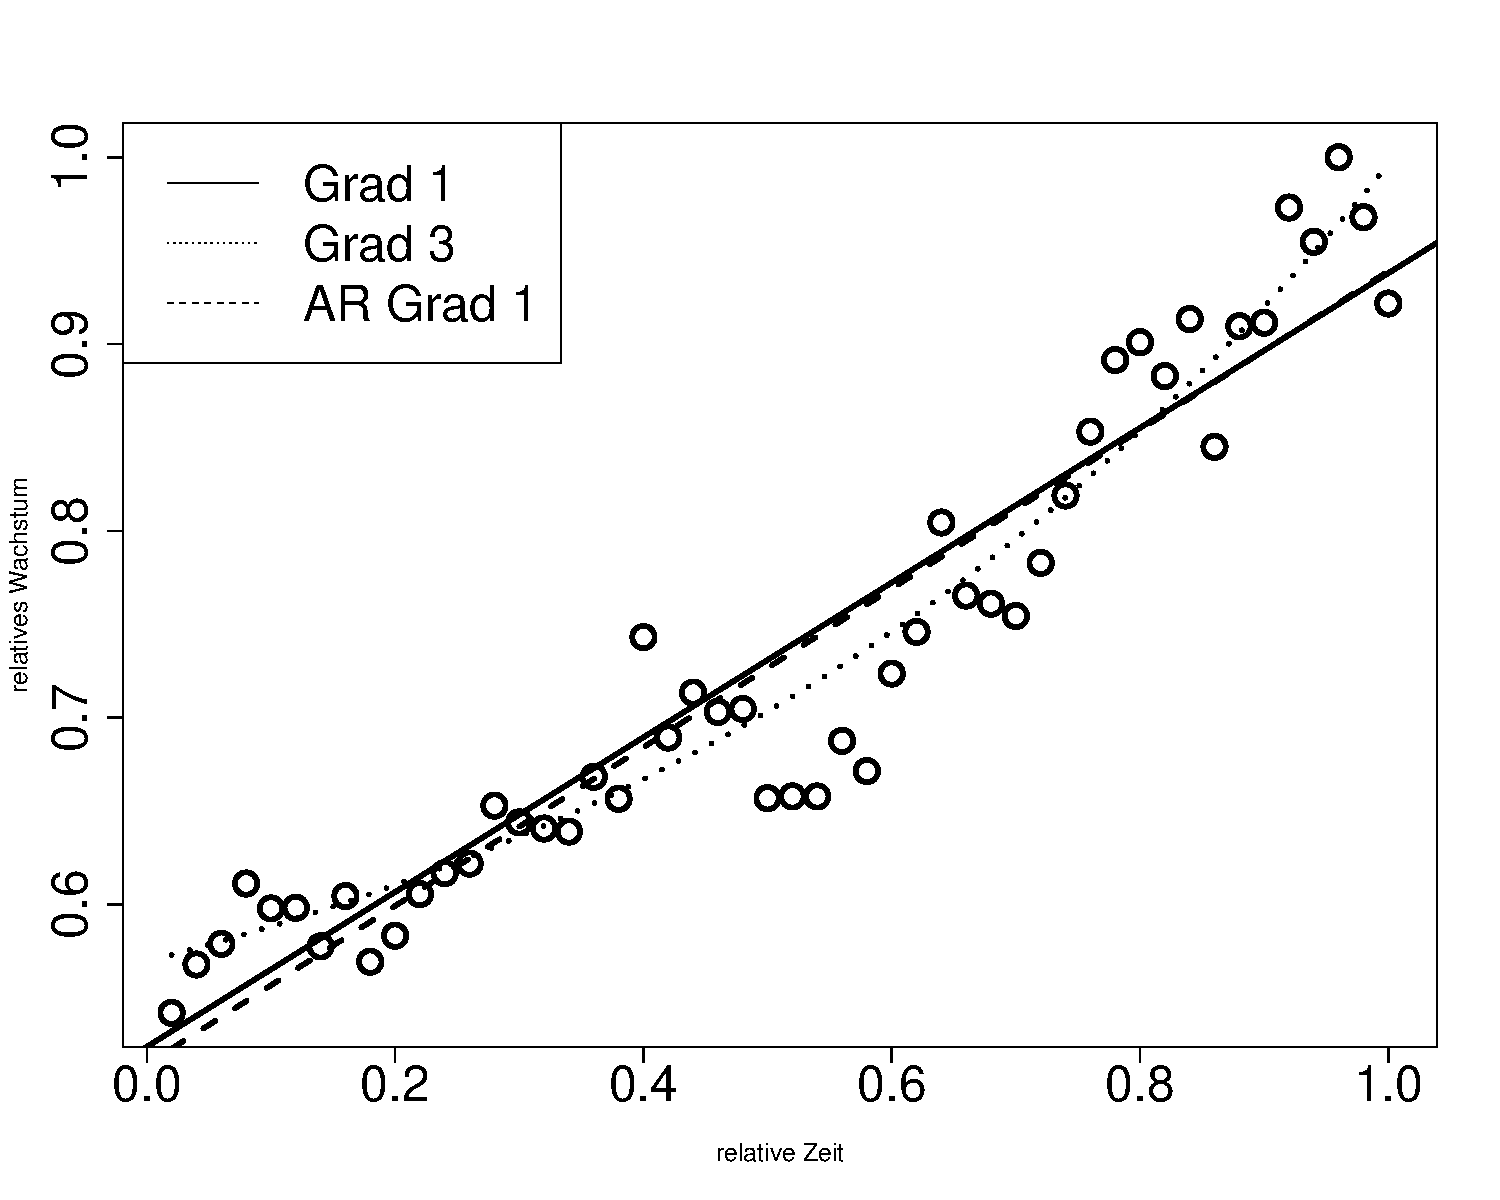
\includegraphics[width=0.5\textwidth]{Bsp-Reg-AR}
  \caption{Regression für AR(1)}
  \label{BSP-Reg-AR}
\end{figure}

Man sieht, dass auch in diesem Fall ein deutlicher Unterschied zwischen den beiden Regressionspolynomen besteht.

\end{Beispiel}




\subsection{Konfidenzbänder für AR(1)}
\label{Konfidenzbaender für AR(1)}
Im letzten Abschnitt wurde gezeigt, dass man einen Schätzer für $\beta$ und $\sigma^2$ bei korrelierten Daten erhalten kann, indem man beide Seiten mit der Kovarianzmatrix $\Upsilon$ multipliziert. 

Wie schon gezeigt, ist $e^{*} = (\Upsilon^{-1/2})e \sim \mathscr{N}_{n}(0,I)$. Die Fehler dieses abgeänderten Modells sind also wieder unabhängig verteilt. Das heißt, es können die Ergebnisse aus Kapitel \ref{Regression und Konfidenzbaender} angewendet und ein Konfidenzband $K^{*}$ bestimmt werden, sodass

\begin{align*}
\mathbb{P}(x^{*'} \beta \in K^{*}) = 1 - \alpha
\end{align*}

Da uns allerdings nicht $x^{*'} \beta$ interessiert, sondern $x' \beta$, muss Bedingung an die Menge in $\mathbb{P}()$ mit $\Upsilon^{1/2}$ multipliziert werden. Auf diese Art erhält man dann ein Konfidenzband für das ursprüngliches Modell \eqref{AR Modell}.

Nun betrachten wir, wie dies die Simulation aus Abschnitt \ref{Konfidenzbaenderauf auf einem Intervall für Regressionsmodell mit Polynomgestalt} beeinflusst. Es ändert sich nur die Simulation von $N$.

Im Speziellen wird die folgende Simulation verwendet, um konkret den Wert der kritischen Konstante $c$ bei abhängigen Daten zu bestimmen:

\begin{enumerate}
\item Simuliere $N \sim \mathscr{N}_{n}(0,(\Upsilon^{-1/2}X'\Upsilon^{-1/2}X)^{-1}) = (0,(X^{*'}X^{*})$ und $\hat{\sigma}/\sigma \sim \sqrt{\chi^2_v/v}$ mit $v=n-p-1$.
\item Berechnung von $K_{2h}(T;(X^{*'}X^{*})^{-1};(a,b))$.
\end{enumerate}

Die Berechnung von $K_{2h}(T,\cdot,(a,b))$ läuft analog zu Kapitel \ref{Konfidenzbaenderauf auf einem Intervall für Regressionsmodell mit Polynomgestalt}, da sich die Funktion $K_{2h}(T;\cdot;(a,b))$ nicht ändert.

\begin{Beispiel}
Jetzt wird das Beispiel aus dem ersten Kapitel fortgeführt, indem zu der Regression mit Grad Drei, dem Konfidenzband auf ganz $\mathbb{R}^{p}$, dem auf $A$ und dem auf $A$ für Polynome noch ein Konfidenzband auf $A$ für Polynome unter Berücksichtigung der AR(1)-Struktur bestimmt wird.

\begin{figure}[H] 
  \centering
     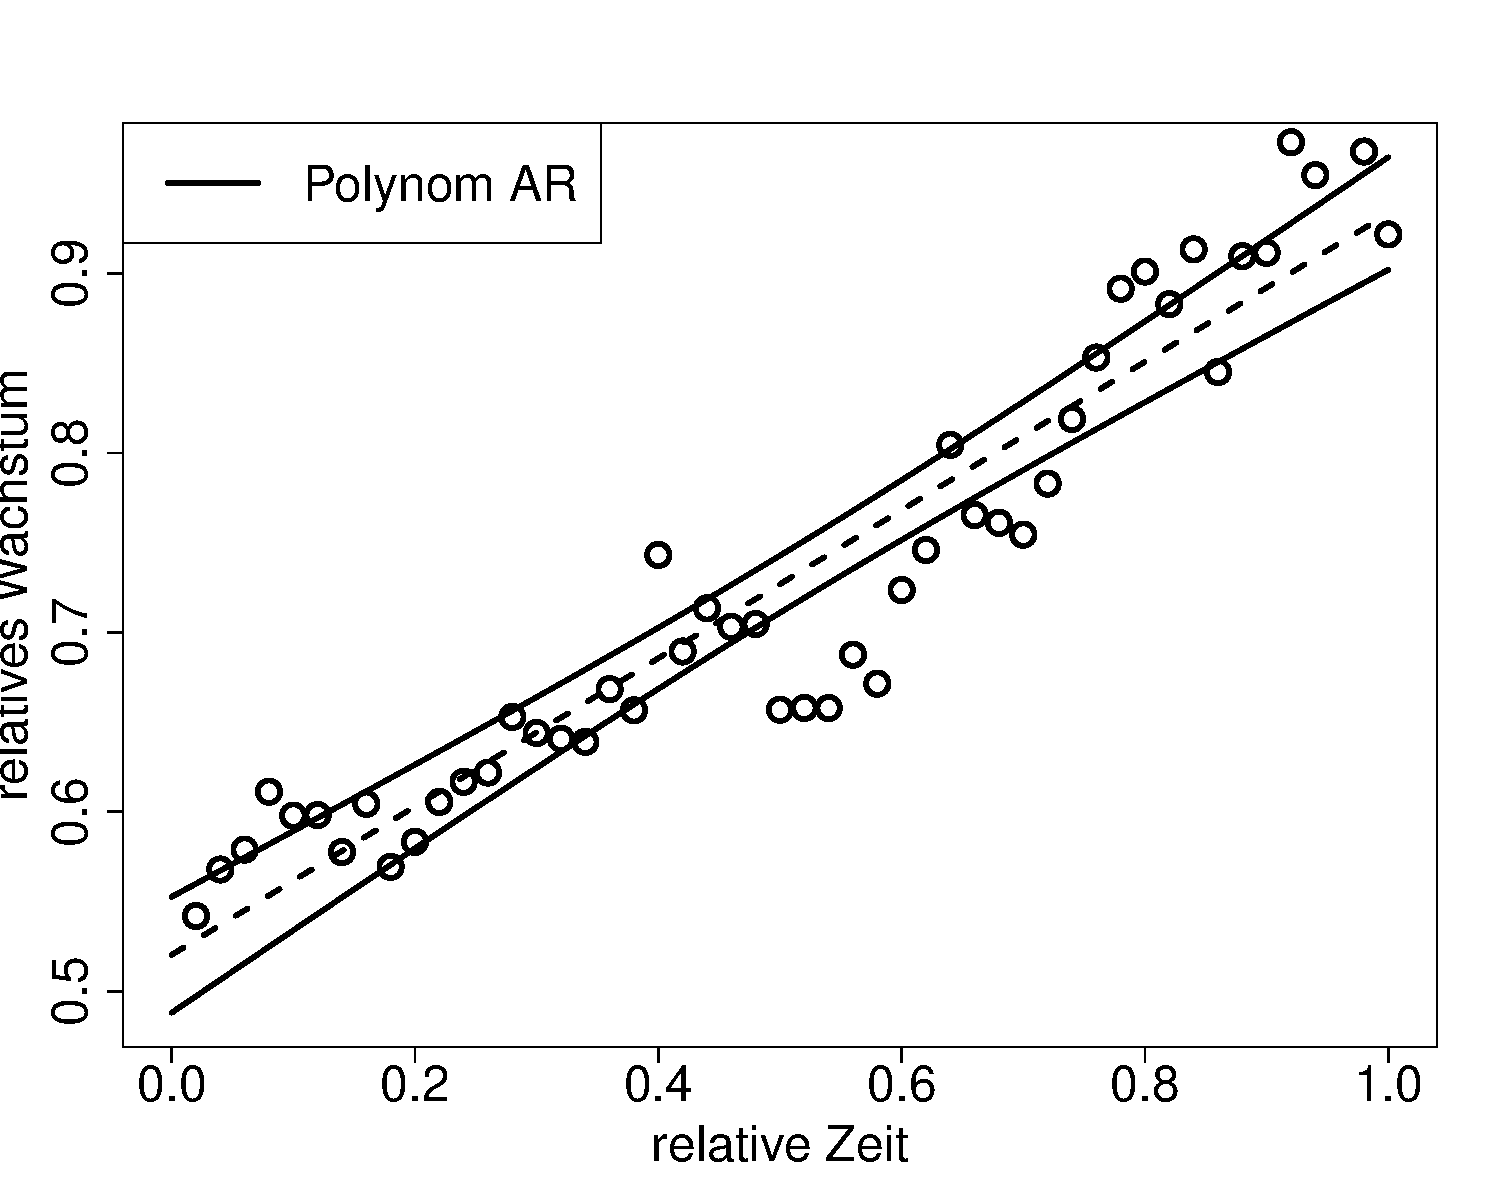
\includegraphics[width=0.5\textwidth]{Bsp-KB-poly-AR}
  \caption{Weiterführung des Beispiels durch Konfidenzband auf $A$ unter Berücksichtigung von Polynomstruktur und AR(1)-Struktur}
  \label{Bsp-KB-poly-AR}
\end{figure}

Man erhält als kritischen Wert für das Konfidenzband auf ganz $\mathbb{R}^{p}$ \cR , für das Konfidenzband auf $A$ \cA, für das Konfidenzband auf $A$ für Polynome \cAP ~und für das Konfidenzband auf $A$ für Polynome das die AR(1)-Struktur berücksichtigt \cAPAR . 

Vergleicht man die Regression mit Grad Drei und mit Grad Vier erhält man die Abbildung \ref{Bsp-KB-poly-hetero-AR}.

\begin{figure}[H] 
  \centering
     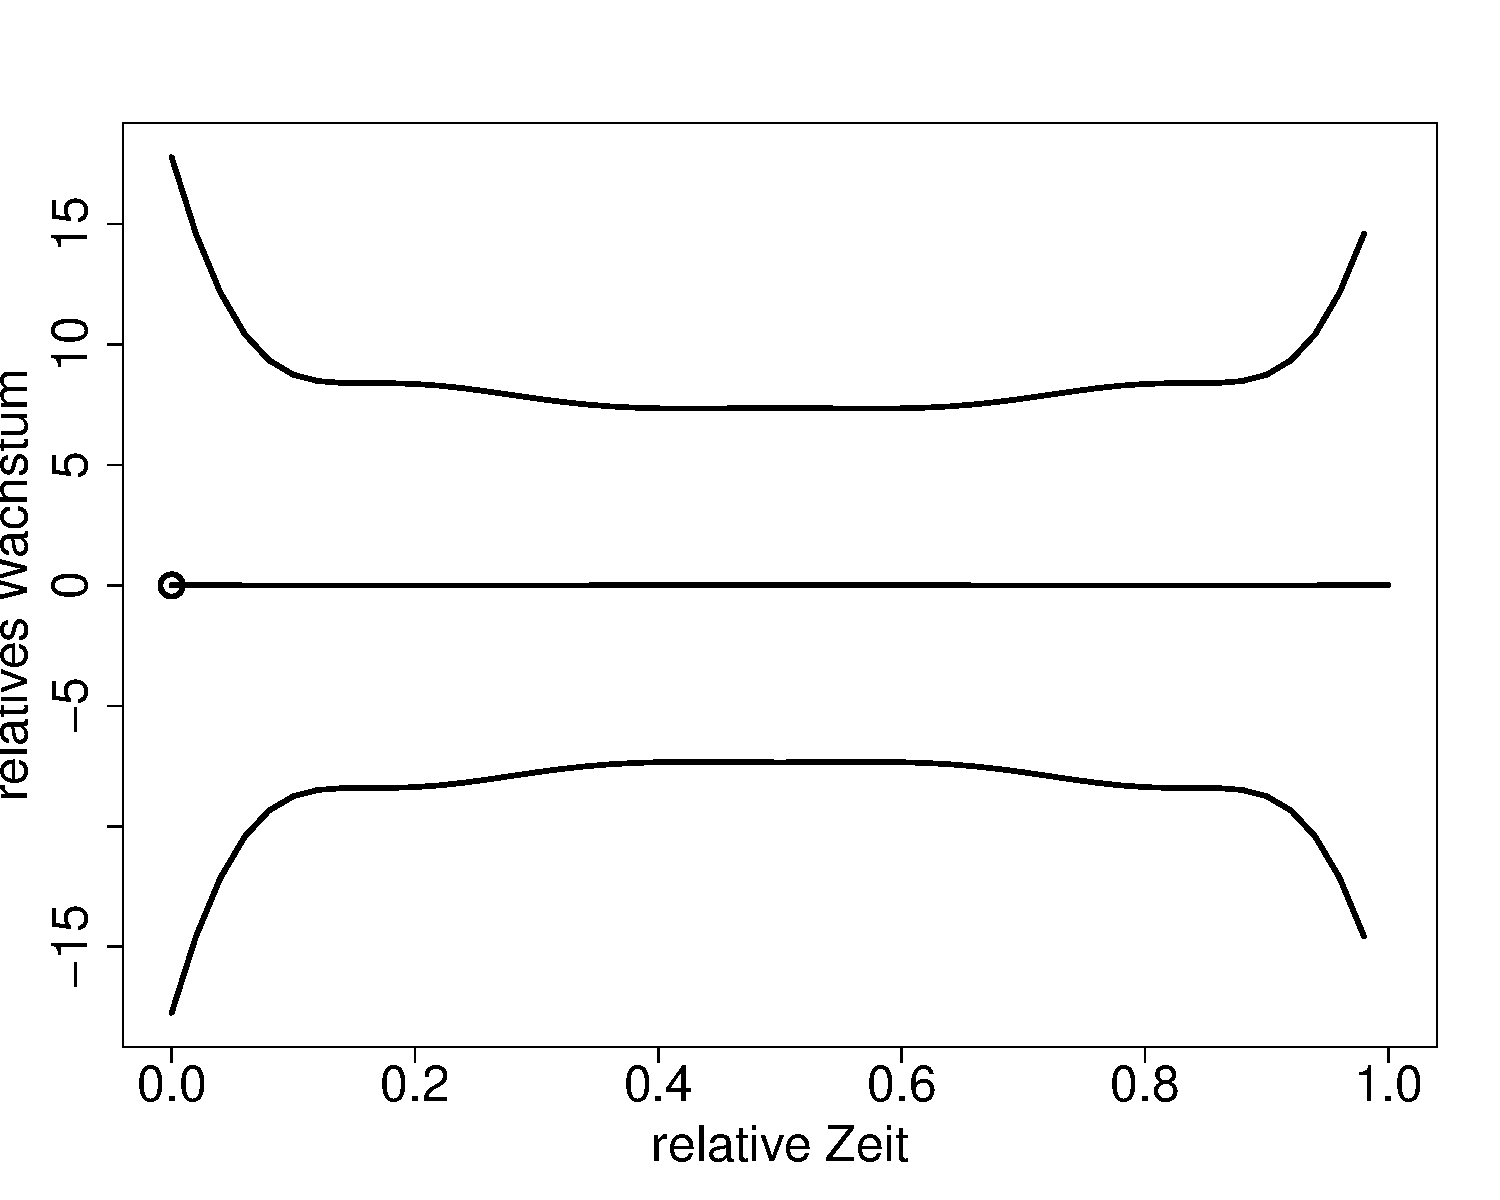
\includegraphics[width=0.5\textwidth]{Bsp-KB-poly-hetero-AR}
  \caption{Vergleich Regression Grad Drei und Grad Vier unter Berücksichtigung der Polynomstruktur und AR(1)-Struktur}
  \label{Bsp-KB-poly-hetero-AR}
\end{figure}

%Man sieht, dass das Konfidenzband weit von den Daten entfernt ist. Vermutlich liegt dies daran, dass $X'X$ in diesem Fall Eigenwerte nahe Null hat. Dadurch führt die Berechnung von $(X'X)^{-1}$ zu seltsamen Ergebnissen.

\end{Beispiel}





\newpage
\section{Datenbeschreibung und Resultate}
\label{Datenbeschreibung und Resultate}
In diesem Kapitel werden zuerst die Daten beschrieben, die als Motivation für die bisher erklärten Methoden dienen. Danach werden die Methoden auf die Daten angewendet. Zuerst werden die verschiedenen Methoden Konfidenzbänder zu bestimmen verglichen. Danach werden Polynommodelle von verschiedenem Grad miteinander verglichen. Die Daten entstammen der Arbeit von \cite{Rehfeldt10}.

Die zur Berechnung der Parameter $\beta$ und  $\sigma$ sowie der kritischen Werte $c_{\mathbb{R}}, c_{A}, c_{AP}$, und zum erzeugen der Abbildungen verwendeten R Skripte können unter 

\begin{center}
\textit{https://github.com/fake1884/KBminmaxpoly} 
\end{center}

eingesehen werden. Eine Übersicht über die verwendeten Skripte befindet sich in der dem R Paket beiliegenden \textit{README.md} Datei in oben genanntem Verzeichnis.

Dabei bezeichnet $c$ immer einen kritischen Wert für die Konstruktion von Konfidenzbändern und der Index bestimmt, um welchen kritischen Wert es sich handelt. Dabei steht $\mathbb{R}$ für ein Konfidenzband auf ganz $\mathbb{R}^{p}$, $A$ steht für ein Konfidenzband auf einer Region $A \subset \mathbb{R}^{p}$ und $AP$ steht für ein Konfidenzband auf einer Region $A \subset \mathbb{R}^{p}$ mit einem polynomiellen Regressionsmodell.

Es stellt sich in diesem Kapitel häufig die Frage, ob die Nullfunktion in einem bestimmten Konfidenzband enthalten ist. Diese Frage wurde immer durch hinschauen entschieden, da die Unterschiede recht groß sind. Sollte eine genauere Auswertung nötig sein, kann die Funktion \textit{Test.function} verwendet werden, die bei den Simulationen geprüft hat, wie oft das wahre Modell im Konfidenzband liegt.

\subsection{Datenbeschreibung}
Die Motivation dieser Arbeit ist, wie eine Stammzelle entscheidet, zu welcher Art Gewebe sie wird. Es wird vermutet, dass Stammzellen diese Entscheidung treffen, wenn sie gerade nicht wachsen. Deshalb wurden Stammzellen auf verschiedene Untergründe gesetzt und zu jeweils bestimmten äquidistanten Zeitpunkten unter einem Mikroskop fotografiert. Danach wurde ihre Fläche bestimmt. Mit Hilfe dieser Daten wird eine Regression mit der Zeit als unabhängige Variable durchgeführt. Es wird eine Polynomregression verwendet, da die Ableitungen von Polynomen gut zu berechnen sind und man so die kritischen Punkte des Regressionsgraphen einfach bestimmen kann.

Es geht darum, das beste Polynom-Modell für die Daten zu wählen. Ein Polynom-Modell ist durch den Grad des Polynoms eindeutig definiert. Das Problem ist also den besten Polynomgrad zu finden.

Um dieses Problem zu lösen, betrachtet man, ob sich die Polynome statistisch signifikant unterscheiden. Dazu schaut man die Differenz der Polynome an und berechnet für diese gleichmäßige Konfidenzbänder. Ist die Nullfuktion vollständig in diesem Konfidenzband enthalten, ist es nicht möglich eine Aussage über den Unterschied der Modelle zu machen. Liegt die Nullfunktion allerdings nicht vollständig im Konfidenzband so, ist der Unterschied signifikant.

Die konkrete Fragestellung meiner Bachelorarbeit ist, ob die Polynome, die man durch die Daten legt, sich signifikant unterscheiden.

Es gibt zwei verschieden Datensätze. Zum einen gibt es einen Datensatz mit Stammzellen, die auf eine Oberfläche mit einer Härte von 10 kPa gesetzt wurden. Zum anderen gibt es einen Datensatz aus Stammzellen, die auf eine Oberfläche von 30 kPa gesetzt wurden. 

Es handelt sich um Daten von 53 Stammzellen bei den 30 kPa Daten und um 51 Stammzellen bei den 10 kPa Daten. An jeder Stammzelle wurde 145 Mal die Größe gemessen. Da die Fläche der Stammzellen für jede einzelne Stammzelle stark schwankt, wird der Mittelwert der Flächen gebildet.

Plottet man nun das Mittel der relative Wachstüme $Y$ gegen die relative Zeit von Null bis Eins mit Schrittweite 1/Anzahl an Beobachtungen, entstehen die Abbildungen \ref{10kPa-data} und \ref{30kPa-data}. 

\begin{figure}[H] 
  \centering
     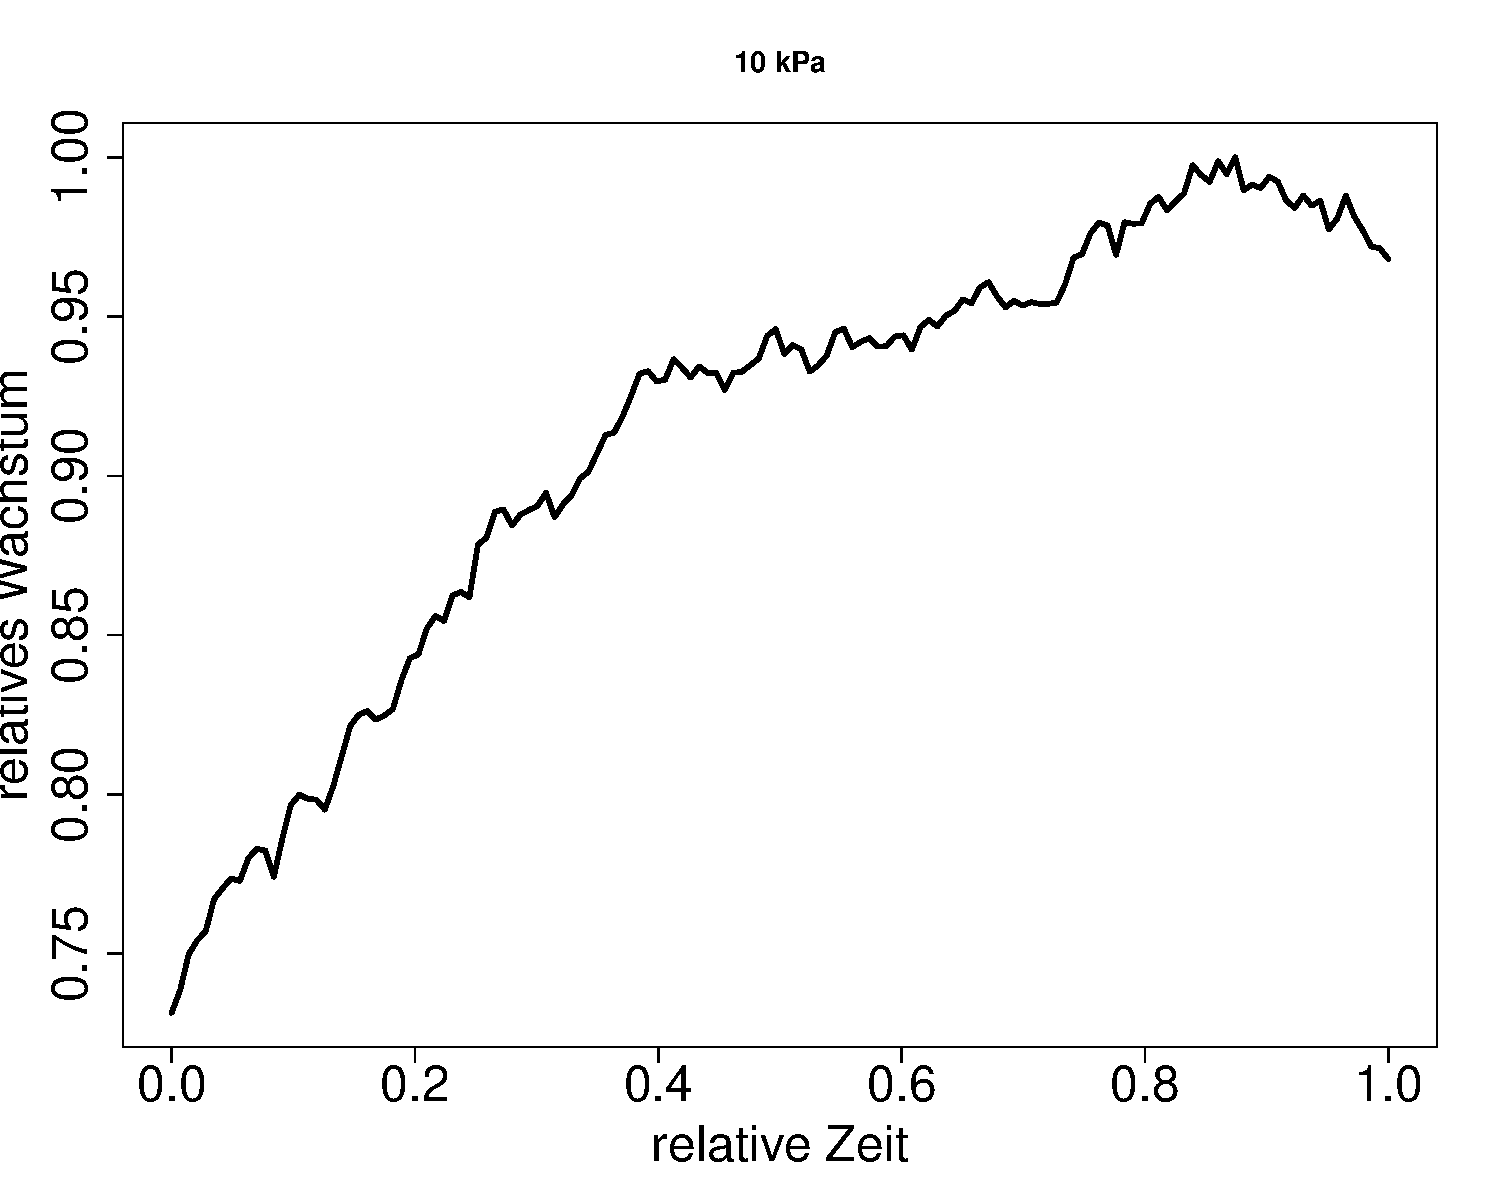
\includegraphics[width=0.5\textwidth]{10kPa-data.pdf}
  \caption{10 kPa Daten}
  \label{10kPa-data}
\end{figure}

\begin{figure}[H] 
  \centering
     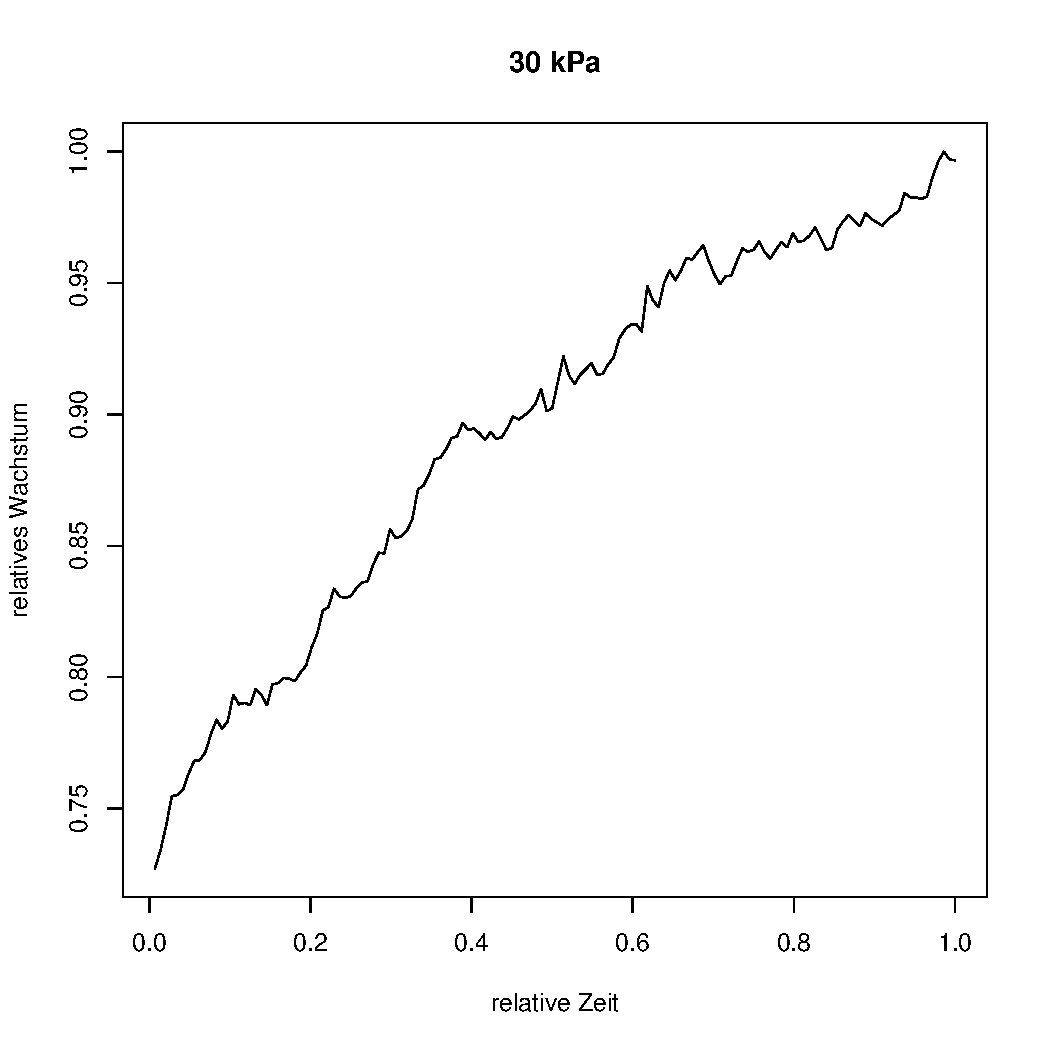
\includegraphics[width=0.5\textwidth]{30kPa-data.pdf}
  \caption{30 kPa Daten}
  \label{30kPa-data}
\end{figure}

Man sieht, dass die Stammzellen in beiden Fällen im Zeitverlauf wachsen. Dabei scheinen die 10 kPa Stammzellen im Zeitintervall [0.1,0.4] schneller zu wachsen, als die 30 kPa Stammzellen. Dafür flacht sich das Wachstum im späteren Zeitverlauf bei den 10 kPa Stammzellen im Vergleich zu den 30 kPa Stammzellen wieder etwas ab.



\subsection{Vergleich verschiedener Konfidenzbänder}
\label{Vergleich verschiedener Konfidenzbänder}
In diesem Abschnitt werden die drei Typen von Konfidenzbändern sowohl für 30 kPa als auch für 10 kPa Daten miteinander verglichen. 

Wir gehen an dieser Stelle davon aus, dass es zwischen den Daten eine Autokorrelationsbeziehung der Art AR(1) gibt. Das bedeutet, zwischen der mittleren Fläche der Stammzellen zum Zeitpunkt $i$ und $i-1$ gibt es folgende Beziehung

\begin{equation*}
y_i = \phi y_{i-1} + e_i
\end{equation*}

mit $e_i$ u.i.v., $\mathbb{E}(e_i)=0$ und $\mathbb{E}(e_i) = \sigma_e^2 < \infty$.

Also muss man die Ergebnisse aus Kapitel \ref{Regression und Konfidenzbänder für abhaengige Daten} anwenden. Das Regressionsmodell ist ein Polynom vom Grad Fünf. Das heißt, $X$ ist die $53 \times 5$ Matrix mit der $l$-ten Zeile von der Form 

\begin{equation*}
\tilde{x}_l = (1, x, x^2, x^3, x^4, x^5 ) \text{ mit } x \in \{0, 1/145, 2/145, \ldots, 144/145, 1 \}
\end{equation*}

Klarerweise ist dann $\beta = (1, \beta_1, \beta_2, \beta_3, \beta_4, \beta_5)$ der gesuchte Koeffizientenvektor und sein Schätzer ist $\hat{\beta} = (1, \hat{\beta_1}, \hat{\beta_2}, \hat{\beta_3}, \hat{\beta_4}, \hat{\beta_5})$. Analoges gilt für $\sigma$ und $\widehat{\sigma^2}$.

Insgesamt gehen wir also von dem folgenden Regressionsmodell aus, wobei die oben eingeführten Bezeichnungen benutzt werden:

\begin{equation*}
Y = X \beta + e
\end{equation*}

mit $e \sim \mathscr{N}_{53}(0, \sigma^2 \Upsilon)$. Dabei ist $\Upsilon$ die von dem zugrunde liegendem AR(1)-Prozess erzeugte Korrelationsmatrix \eqref{Upsilon}

\begin{equation*}
\Upsilon = 
\left[
   \begin{array}{cccccc}
     1 				& \phi 			& \phi^2	& \cdots	& \phi^{n-2}	& \phi^{n-1} 	\\
     \phi 			& 1		 		& \phi 		& \cdots	& \phi^{n-3}	& \phi^{n-2} 	\\
     \phi^2 		& \phi 			& 1		 	& \ddots	& \vdots		& \vdots 		\\
     \vdots		 	& \vdots	 	& \ddots	& \ddots	& \phi			& \phi^{2} 	\\
     \phi^{n-2} 	& \phi^{n-3}	& \cdots 	& \phi		& 1				& \phi 		\\
     \phi^{n-1} 	& \phi^{n-2} 	& \cdots	& \phi^{2}	& \phi			& 1  
   \end{array}
\right]
\end{equation*}

die wir bereits aus Kapitel \ref{Regression für AR(1)} kennen. 

Die Matrix $\Upsilon$ wird durch den Parameter $\phi$ bereits vollständig charakterisiert. Der Schätzer für $\phi$ wird mit $\hat{\phi}$ bezeichnet.

Bei den beiden Simulationen für $c_{A}$ und $c_{AP}$ werden jeweils 250 Iterationen durchgeführt.

Bei den Simulationen auf $A$ für das Modell mit Polynomgestalt wird ein Gridsearch für das Maximum mit Feinheit 145, also der Anzahl an Messungen durchgeführt.

Führt man diese Regression durch, erhält man die Schätzer für die 30 kPa Daten 

\begin{eqnarray*}
\hat{\beta} &=& (0.7287814 ;  0.7345406 ; -2.1593520 ;  5.2097479 ; -5.9029071 ;  2.3863759) \\
\widehat{\sigma^2} &=& 0.009266163 \\
\hat{\phi} &=& 0.9039573 
\end{eqnarray*}
Als kritische Parameter erhält man $c_{\mathbb{R}} = 3.604075, c_{A} = 3.505922$ und $ c_{AP} = 2.902647 $. 

Setzt man dasselbe Modell wie oben für die 30 kPa Daten für die 10 kPa Daten, nur mit an, erhält man die Werte 

\begin{eqnarray*}
\hat{\beta} &=& (0.7372386;   0.4218583 ;  1.8729639 ; -7.6991653 ;  9.7892837 ; -4.1541509) \\
\widehat{\sigma^2} &=& 0.007545373 \\
\hat{\phi} &=& 0.8225374 
\end{eqnarray*}

Als kritische Parameter erhält man $c_{\mathbb{R}} = 3.604075, c_{A} = 3.550114, c_{AP} = 2.848484 $. 

Anhand der kritischen Werte sieht man bereits, dass die Interferenz bei dem Konfidenzband auf $A$ für das Polynommodell eindeutig besser ist. Das heißt, der Wert ist kleiner und somit das Konfidenzband schmaler.

Zeichnet man die Regressionsmodelle und die Konfidenzbänder jeweils in eine Abbildung erhält man die beiden Abbildungen \ref{10kPa-method} und \ref{30kPa-method}.

\begin{figure}[H] 
  \centering
     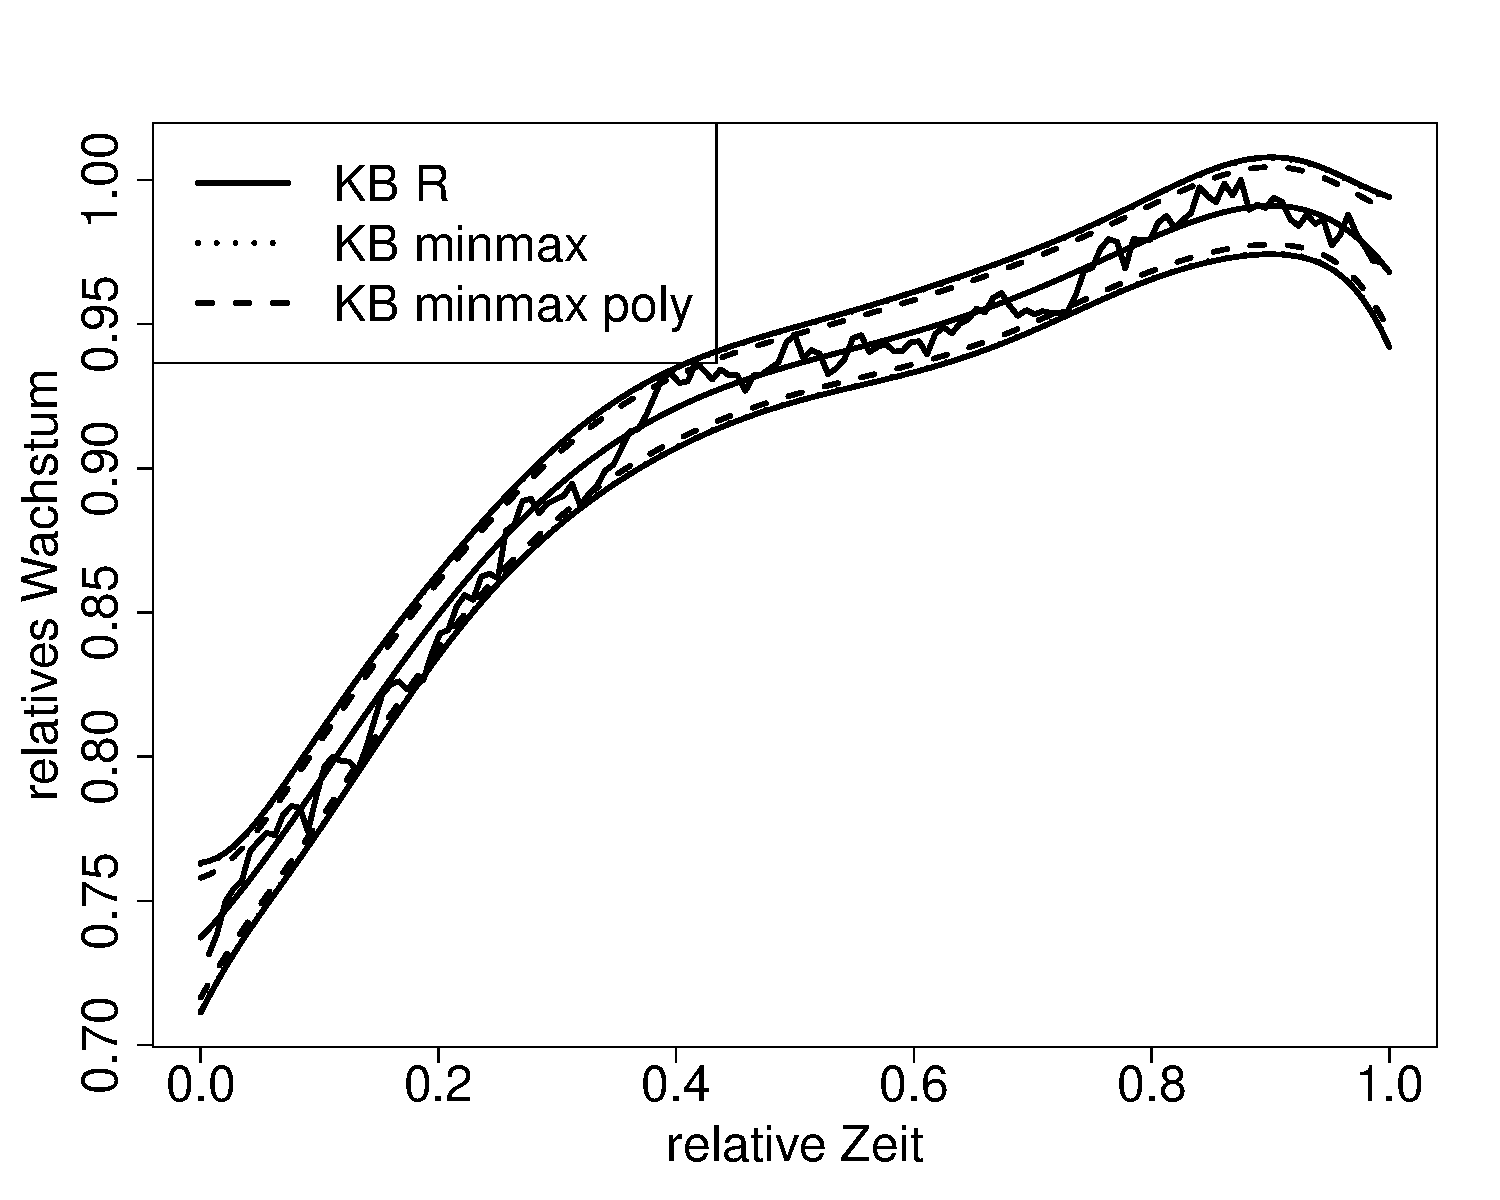
\includegraphics[width=0.65\textwidth]{10kPa-method.pdf}
  \caption{Vergleich von Konfidenzbändern 10 kPa}
  \label{10kPa-method}
\end{figure}

\begin{figure}[H] 
  \centering
     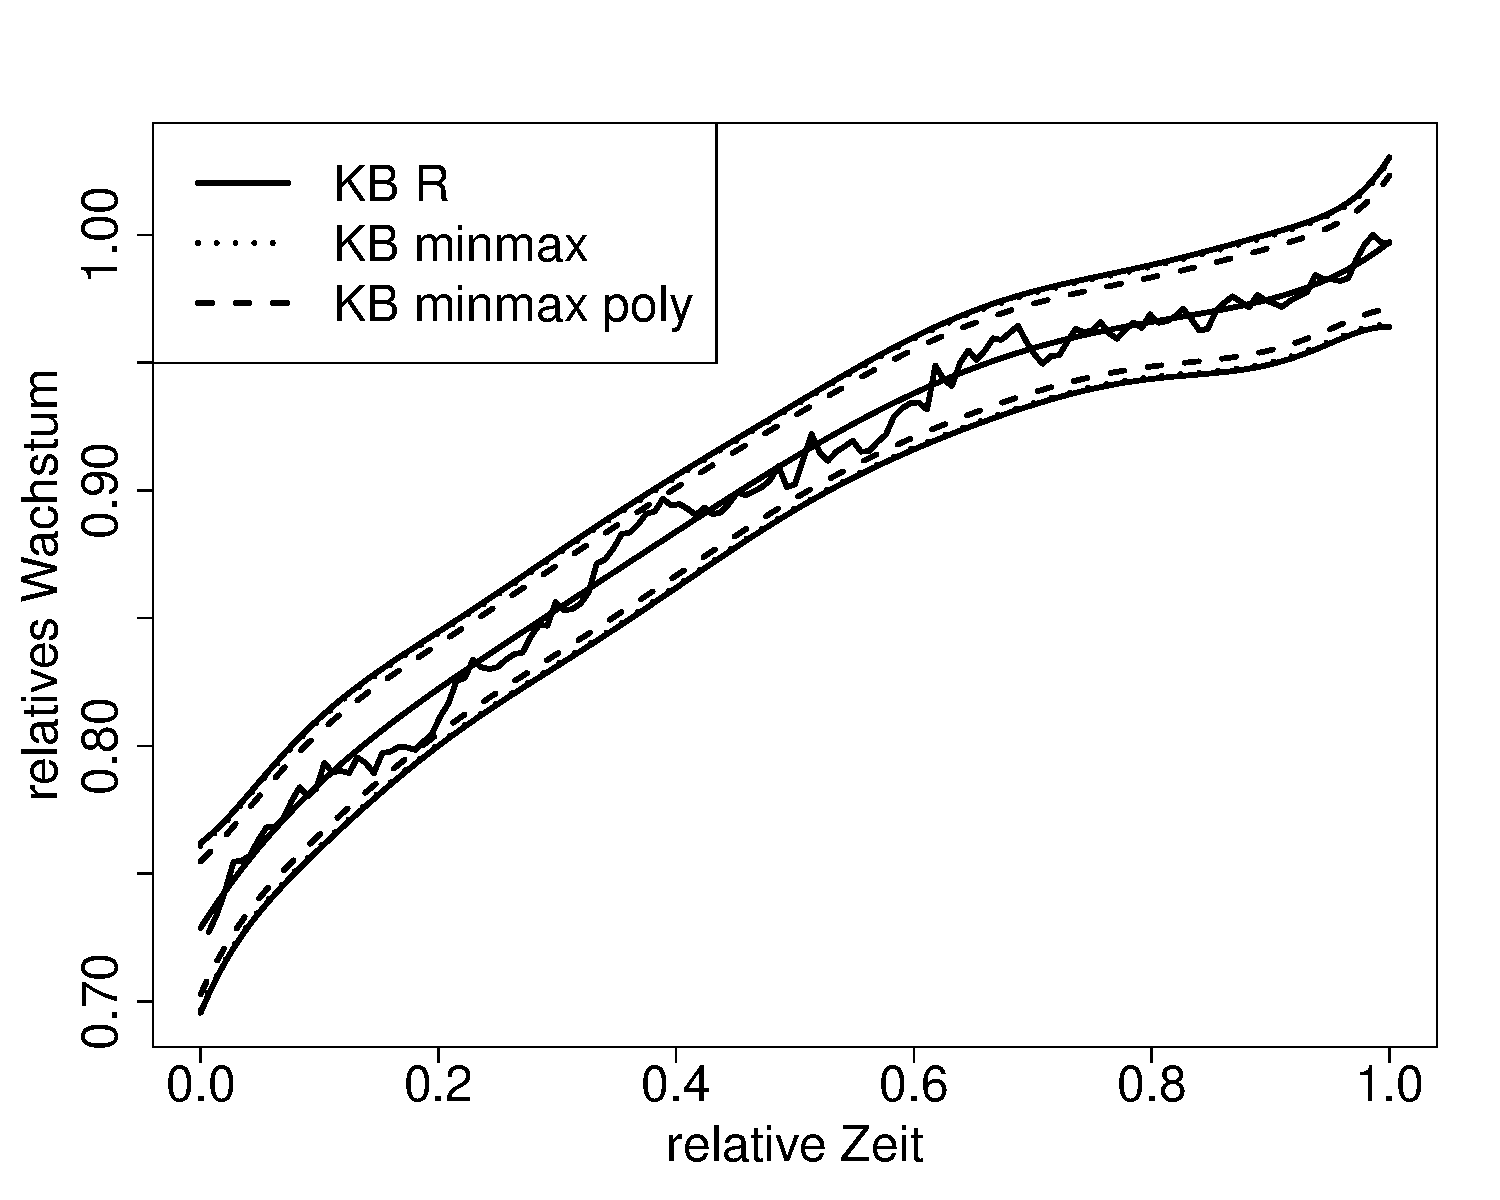
\includegraphics[width=0.65\textwidth]{30kPa-method.pdf}
  \caption{Vergleich von Konfidenzbändern 30 kPa}
  \label{30kPa-method}
\end{figure} 

Man sieht, dass  das Konfidenzband auf $A = [0,1] \subset \mathbb{R}^{p}$, das die Polynomstruktur berücksichtigt, erkennbar schmaler ist. Zwischen den anderen beiden Konfidenzbänder ist kein Unterschied erkennbar.




\subsection{Vergleich von polynomen Regressionsmodellen mit  Grad Vier, Fünf und Sechs}
Ziel dieses Abschnittes ist es zu testen, ob Polynomregressionen von verschiedenem Grad für die beiden Stammzelldatensätze sich statistisch signifikant unterscheiden.

Das heißt, wir führen Regressionen mit einer Designmatrix $X$ bei der die $l$-te Zeile von $X$ durch $\tilde{x}_l = (1, x, x^2, x^3, x^4)$ gegeben ist durch. Danach führen wir analoge Regressionen für Grad Fünf und Sechs durch.

Dazu wird zuerst die Regression durchgeführt, bevor die Testhypothese formalisiert wird. Als Regressionsmodell wird das Regressionsmodell aus Kapitel \ref{Regression und Konfidenzbänder für abhaengige Daten} 

\begin{equation*}
Y = X \beta + e
\end{equation*}

mit $e \sim \mathscr{N}_n(0, \sigma^2 \Upsilon)$ verwendet. Dabei ist $\Upsilon$ die bekannte von einem AR(1) Prozess erzeugte Korrelationsmatrix, die nur von dem unbekannten Parameter $\phi$ abhängt.

Führen wir für die Regressionen durch erhalten wir für die 10 kPa Daten die folgenden Werte. Dabei steht der Index für den Grad des zugehörigen Polynommodells

\begin{eqnarray*}
\hat{\beta_{4}} &=& (0.7314 ; 0.8401 ; -1.5883 ; 1.8877 ; -0.9029) \\
\hat{\sigma_{4}} &=& 0.4943004 \\
\hat{\phi_{4}} &=& 0.9999575 \\
\cline{2-3}
\hat{\beta_{5}} &=& (0.7372 ; 0.4219 ; 1.8730 ; -7.6992 ; 9.7893 ; -4.1542) \\
\hat{\sigma_{5}} &=& 0.007545373 \\
\hat{\phi_{5}} &=& 0.8225374 \\
\cline{2-3}
\hat{\beta_{6}} &=& (0.7352 ; 0.6265 ; -0.6151 ; 3.0831 ; -11.1962 ; 14.6223 ; -6.2906)  \\
\hat{\sigma_{6}} &=& 0.007205863 \\
\hat{\phi_{6}} &=& 0.8065796
\end{eqnarray*}

und für die 30 kPa Daten die Werte:

\begin{eqnarray*}
\hat{\beta_{4}} &=&  0.7311  0.5245 -0.3546  0.0390  0.0546  \\
\hat{\sigma_{4}} &=& 0.009576459 \\
\hat{\phi_{4}} &=& 0.9090669 \\
\cline{2-3}
\hat{\beta_{5}} &=&   0.7288   0.7345  -2.1594   5.2097  -5.9029   2.3864 \\
\hat{\sigma_{5}} &=& 0.009266163 \\
\hat{\phi_{5}} &=& 0.9039573 \\
\cline{2-3}
\hat{\beta_{6}} &=&   0.7273   0.9495  -4.7664  16.2343 -26.7566  20.5211  -5.9124  \\
\hat{\sigma_{6}} &=& 0.01673707 \\
\hat{\phi_{6}} &=&  0.9701881
\end{eqnarray*}

Plottet man die drei Regressionsmodelle in je eine Abbildung für die beiden Datensätze entstehen die beiden Abbildungen \ref{10kPa-Polynomregressionen} und \ref{30kPa-Polynomregressionen}:

\begin{figure}[H] 
  \centering
     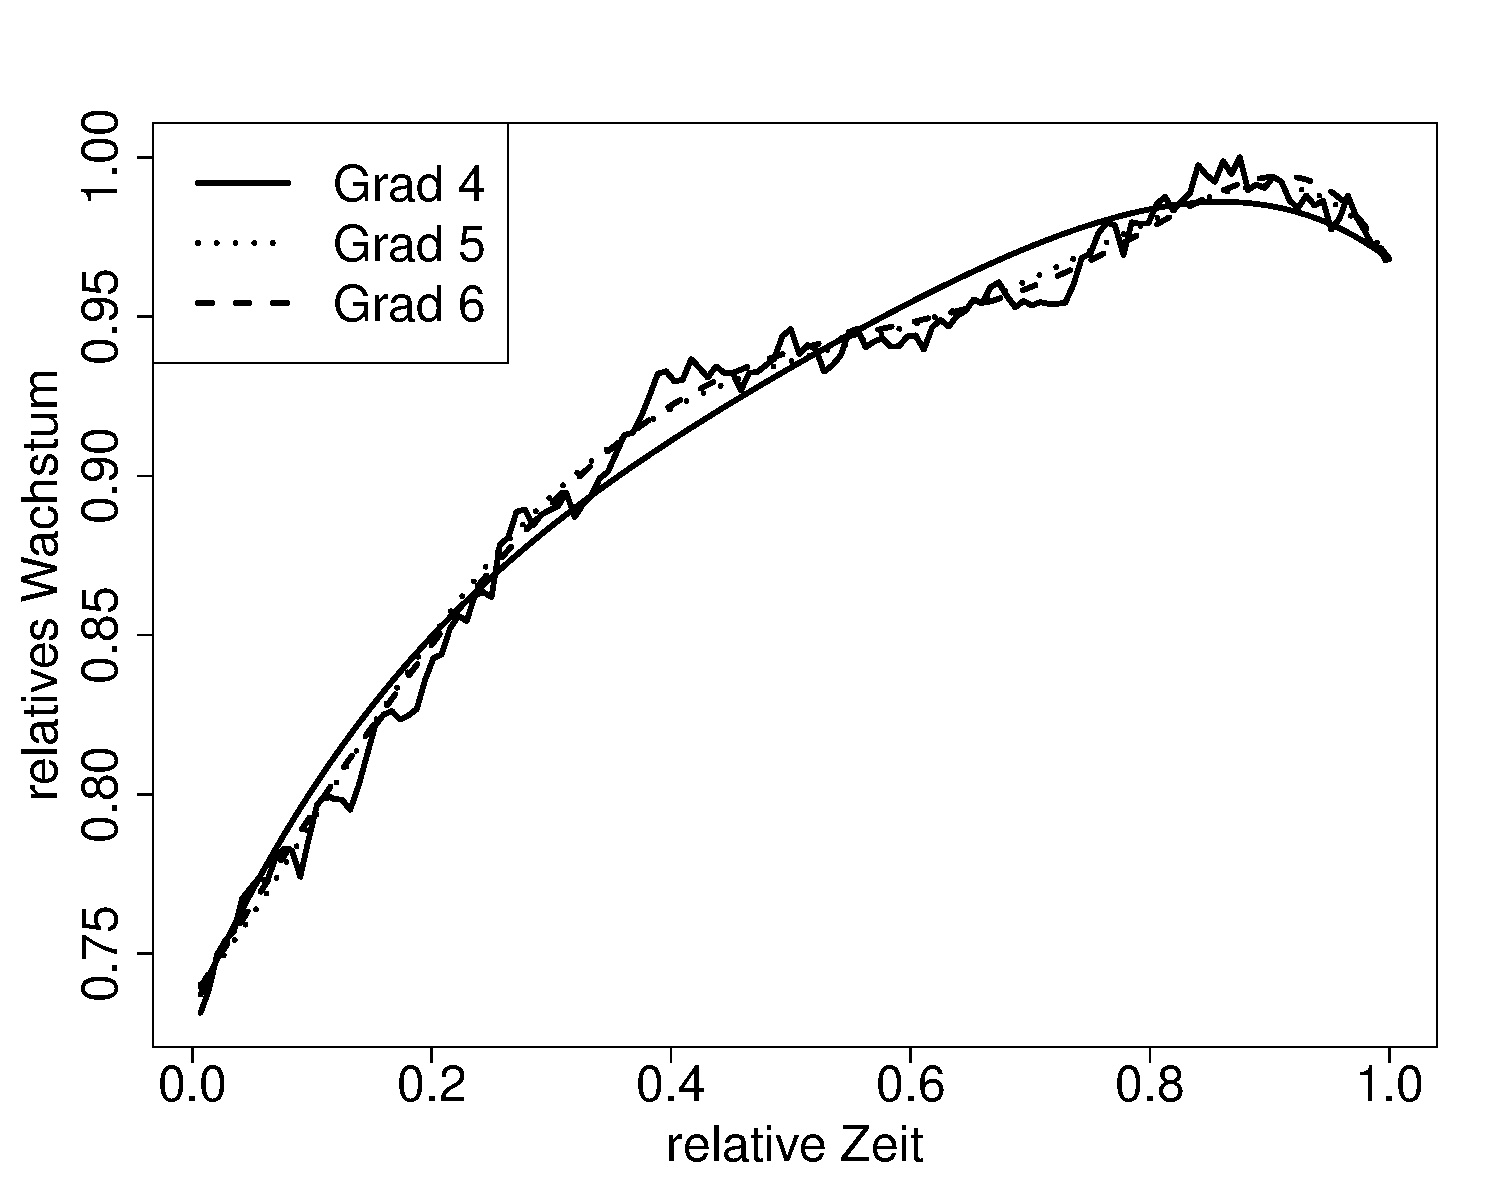
\includegraphics[width=0.65\textwidth]{10kPa-poly.pdf}
  \caption{10 kPa Verschiedene Polynomgrade}
  \label{10kPa-Polynomregressionen}
\end{figure}


\begin{figure}[H] 
  \centering
     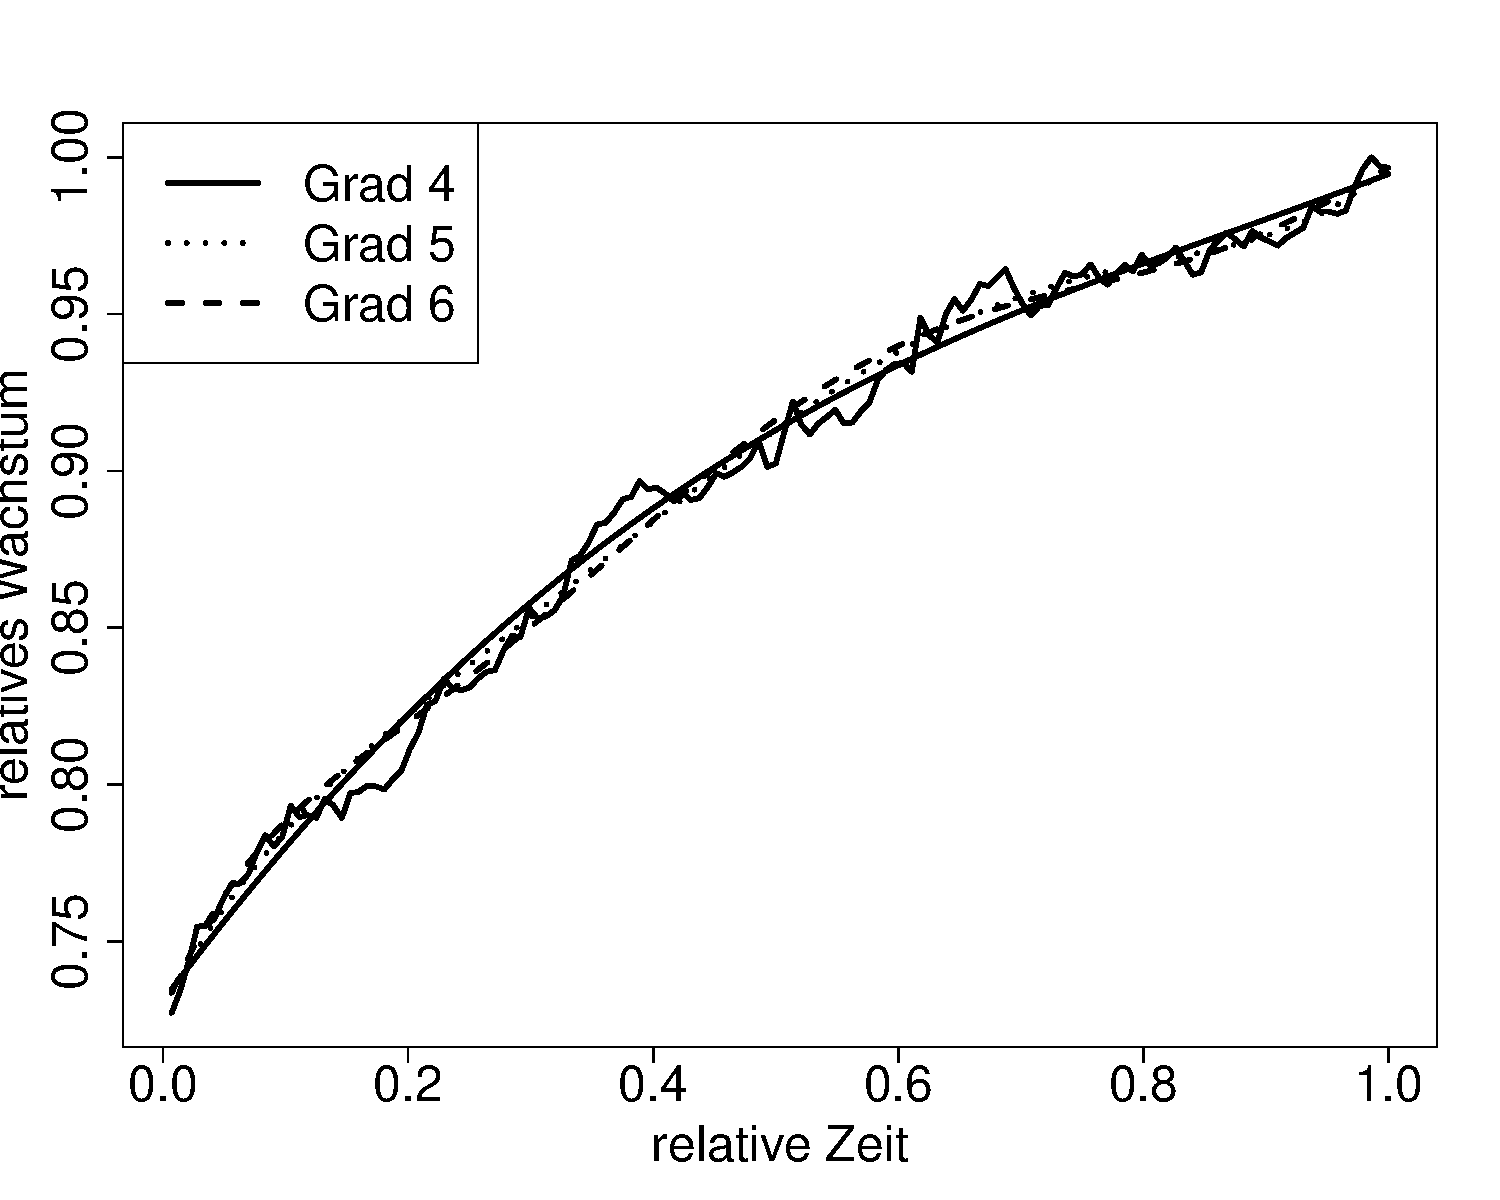
\includegraphics[width=0.65\textwidth]{30kPa-poly.pdf}
  \caption{30 kPa Verschiedene Polynomgrade}
  \label{30kPa-Polynomregressionen}
\end{figure}

Man sieht, dass sich die Regressionsmodelle für die 10 kPa Daten relativ stark unterscheiden, während die Regressionsmodelle bei den 30 kPa Daten fast gleich sind.

Als nächstes testen wir, ob sich die Polynomregressionen von Grad Vier und Grad Fünf unter statistischer Unsicherheit gleich sind. Das heißt, wir testen die Hypothese

\begin{equation*}
H_0 : \beta_{4} = \beta_{5} \textbf{ vs. } \beta_4 \neq \beta_{5}
\end{equation*}

Dazu benutzen wir die Konfidenzbandmethode aus Kapitel \ref{Vergleich von zwei Regressionsmodellen} beziehungsweise ihre Abwandlung aus Abschnitt \ref{Konfidenzbaender für AR(1)}.

Zeichnen wir die Differenz von $\hat{\beta_4}$ und $\hat{\beta_5}$ mit dem zugehörigen Konfidenzband in je eine Abbildung für die beiden Datensätze erhalten wir die beiden Abbildungen \ref{10kPa-Regmod-4-5} und \ref{30kPa-Regmod-4-5}.

\begin{figure}[H] 
  \centering
     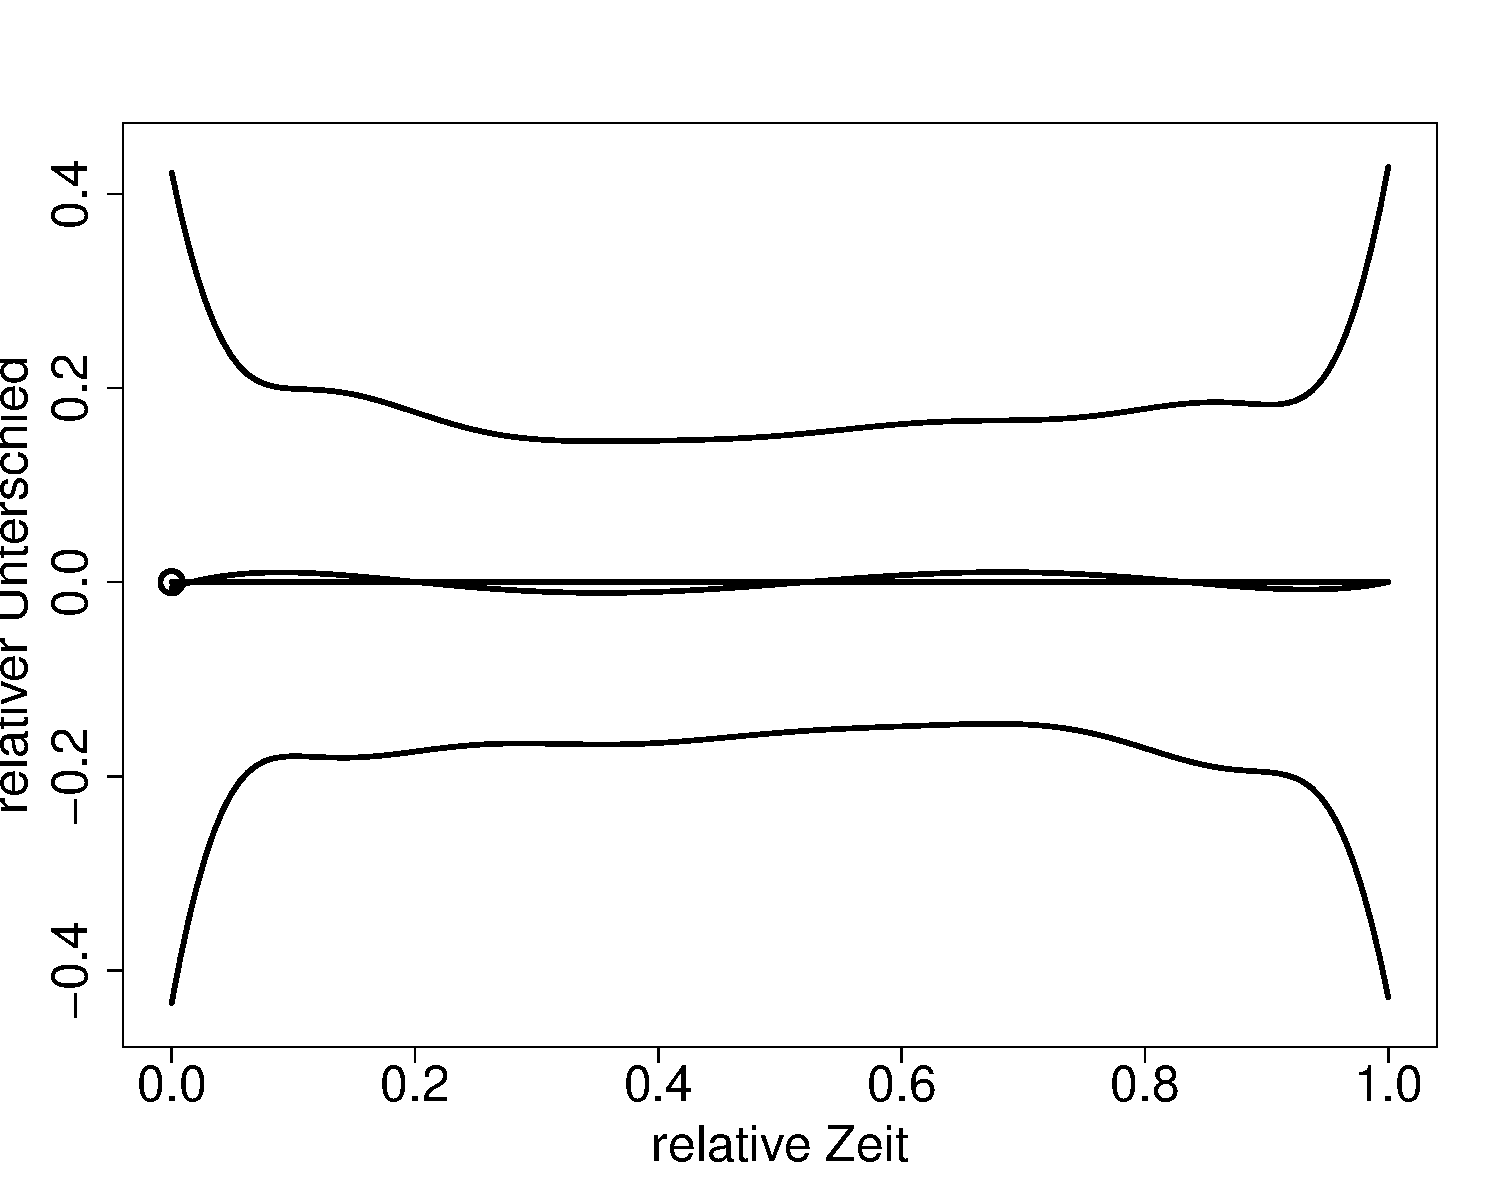
\includegraphics[width=0.5\textwidth]{10kPa-poly-KB-4-5.pdf}
  \caption{10 kPa Vergleich von Regressionsmodellen mit Grad Vier versus Grad Fünf}
  \label{10kPa-Regmod-4-5}
\end{figure}

\begin{figure}[H] 
  \centering
     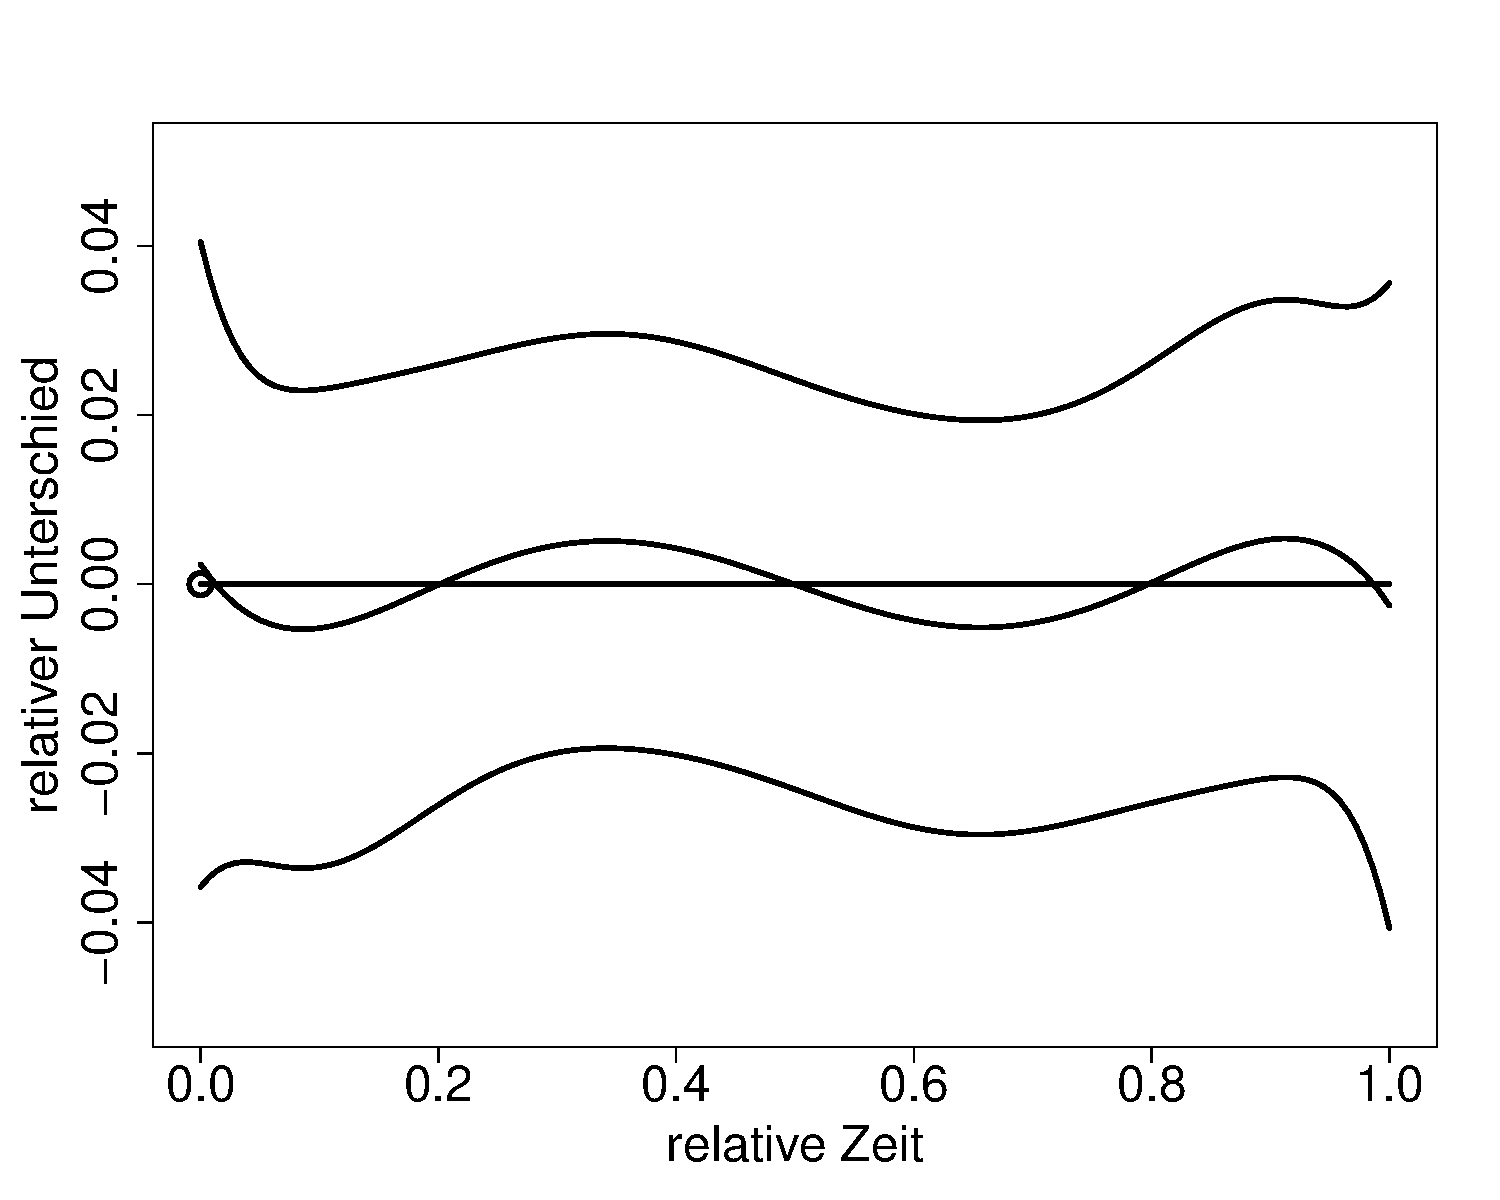
\includegraphics[width=0.5\textwidth]{30kPa-poly-KB-4-5.pdf}
  \caption{30 kPa Vergleich von Regressionsmodellen mit Grad Vier versus Fünf}
  \label{30kPa-Regmod-4-5}
\end{figure}

Wie man sieht, ist in im Fall der 10 kPa Daten die Nullfunktion eindeutig vollständig im Konfidenzband enthalten und wir können die Nullhypothese nicht ablehnen.

Bei den 30 kPa Daten ist die Nullhypothese auch knapp ganz im Konfidenzband enthalten und wir können die Nullhypothese wieder nicht ablehnen.

In den folgenden Vier Abbildungen testen wir die analogen Hypothesen

\begin{eqnarray*}
& H_0 : \beta_4 = \beta_6 & \textbf{ vs. } H_1 : \beta_4 \neq \beta_6 \\
& H_0 : \beta_5 = \beta_6 & \textbf{ vs. } H_1 \beta_5 \neq \beta_6
\end{eqnarray*} 

für die 10 kPa beziehungsweise 30 kPa Daten. Für die Hypothese Grad Vier versus Grad Sechs erhält man die Abbildungen \ref{10kPa-Regmod-4-6} und \ref{30kPa-Regmod-4-6}

\begin{figure}[H] 
  \centering
     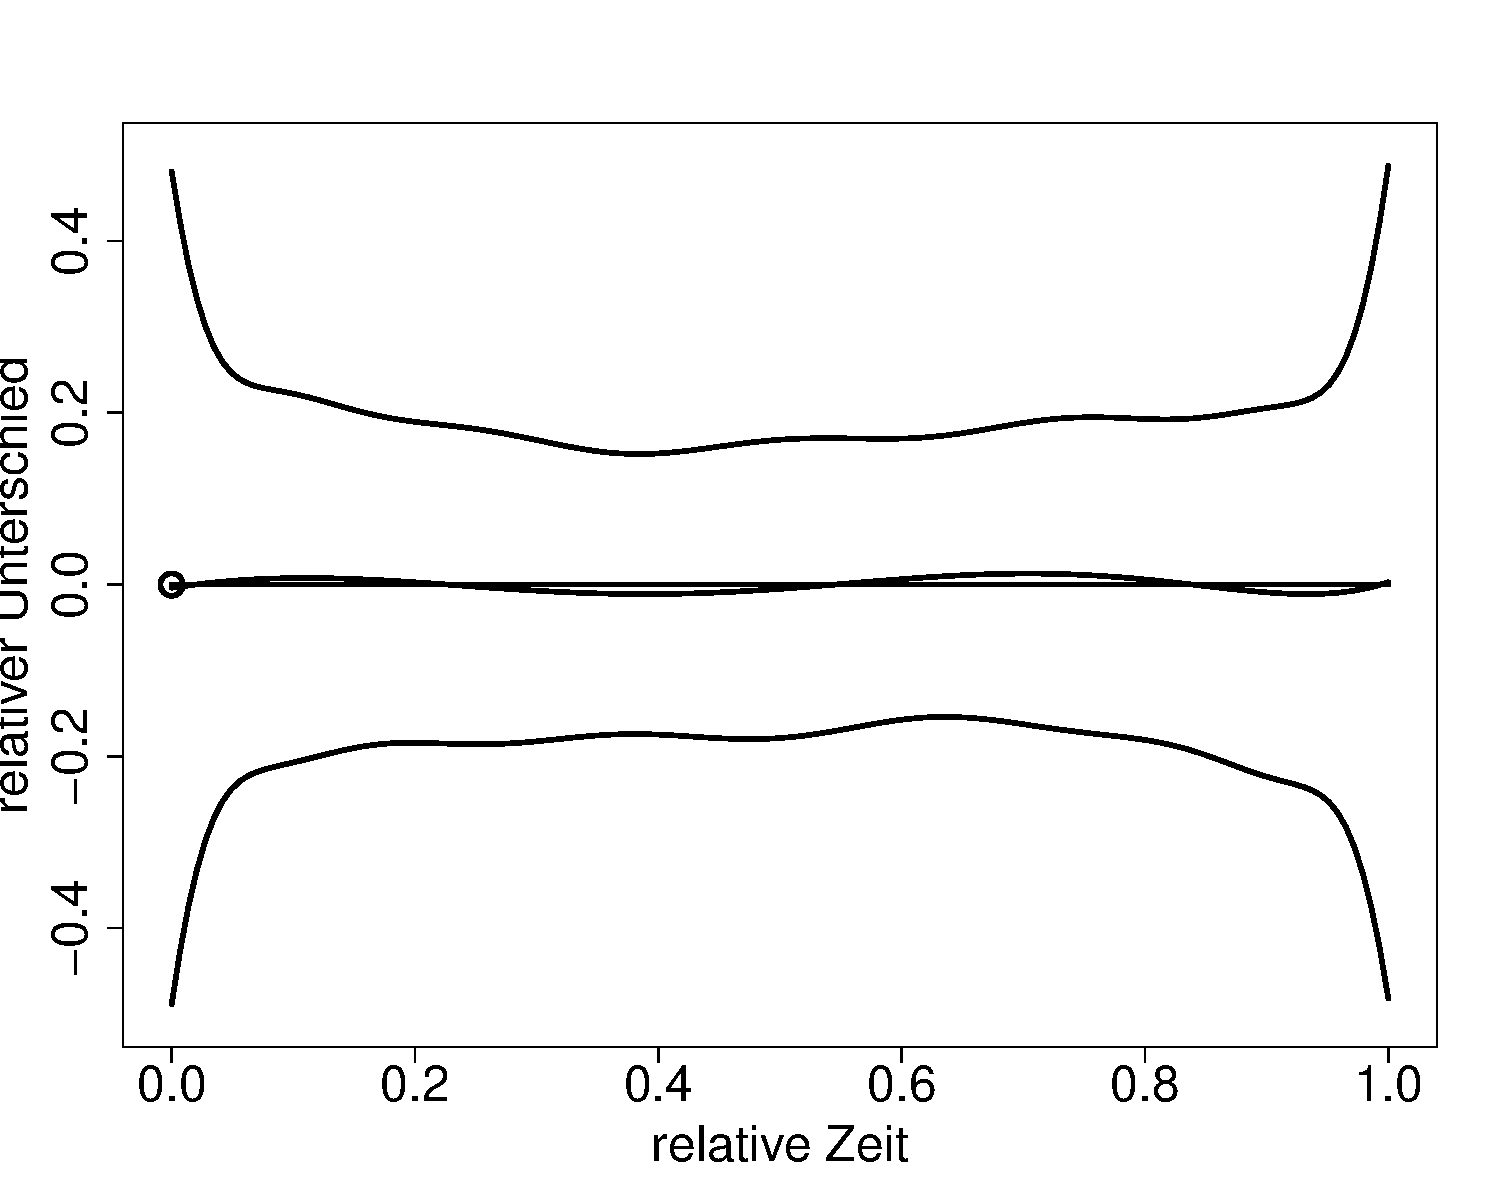
\includegraphics[width=0.5\textwidth]{10kPa-poly-KB-4-6.pdf}
  \caption{10 kPa Vergleich von Regressionsmodellen mit Grad Vier versus Sechs}
  \label{10kPa-Regmod-4-6}
\end{figure}

\begin{figure}[H] 
  \centering
     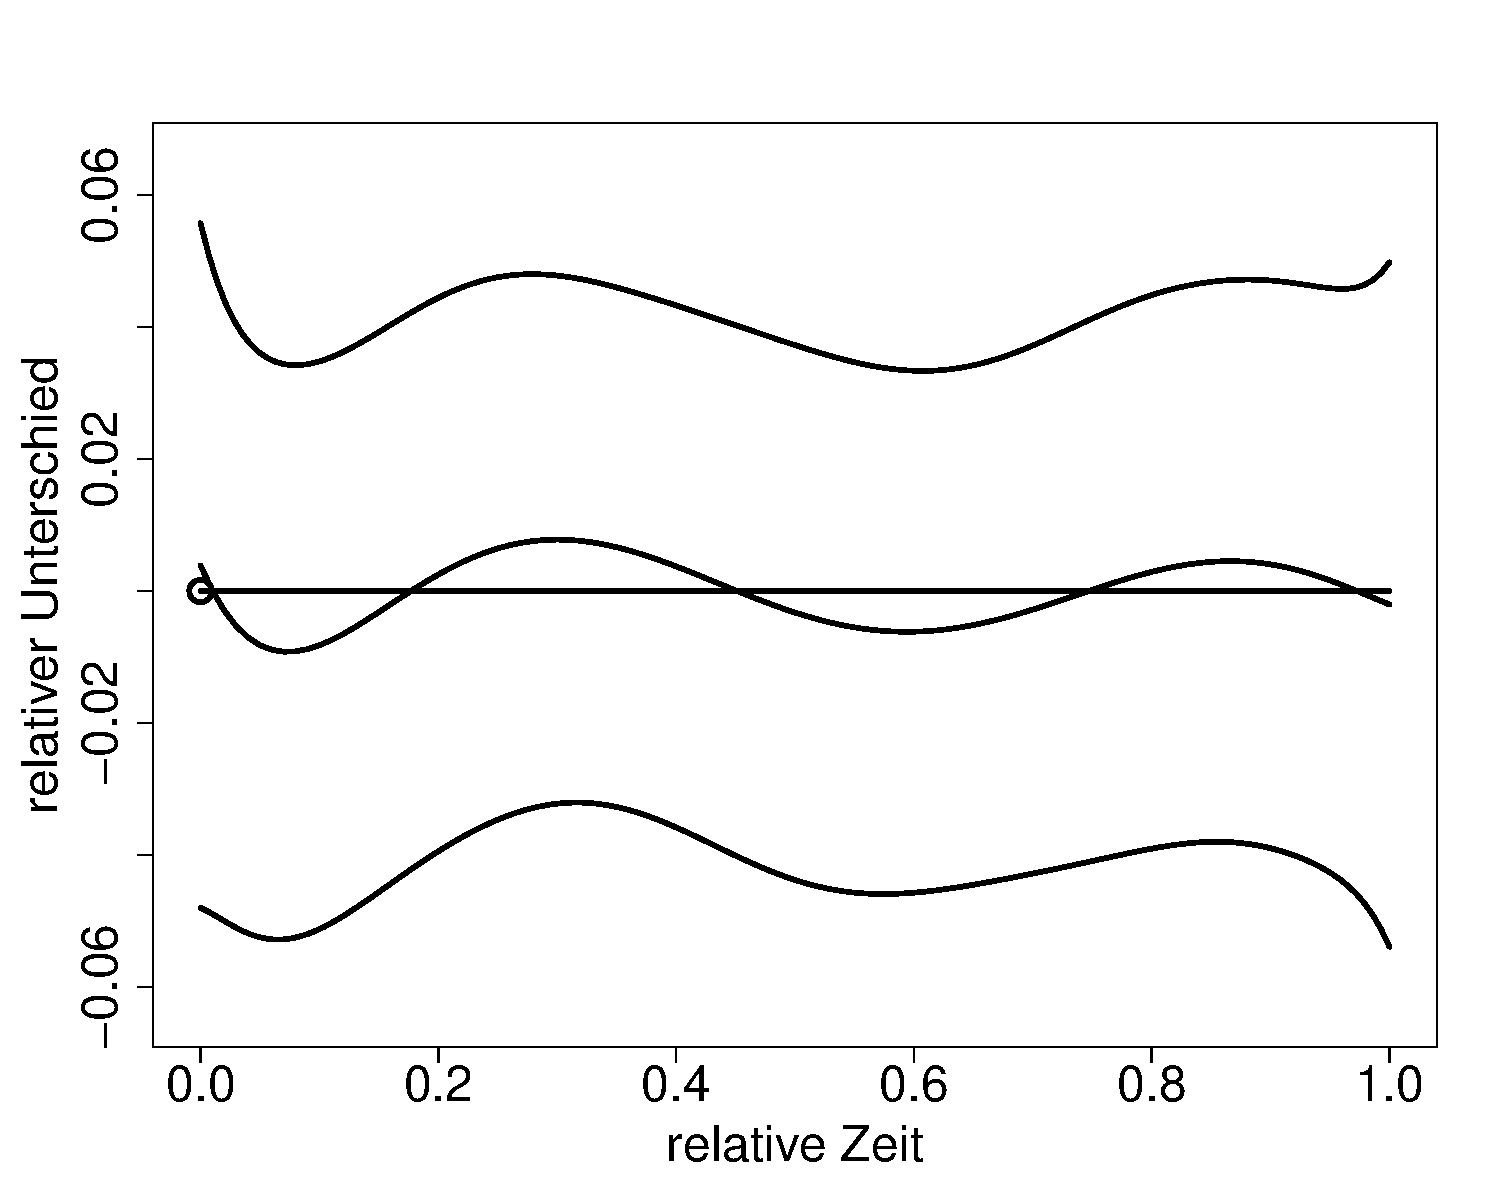
\includegraphics[width=0.5\textwidth]{30kPa-poly-KB-4-6.pdf}
  \caption{30 kPa Vergleich von Regressionsmodellen mit Grad Vier versus Sechs}
  \label{30kPa-Regmod-4-6}
\end{figure}

Man sieht, dass sich der Trend aus den beiden vorherigen Abbildungen wiederholt. Bei den 10 kPa Daten gibt es keinen Zweifel, dass die Nullhypothese nicht abgelehnt werden kann. Bei den 30 kPa Daten kann die Nullhypothese auch eindeutig nicht abgelehnt werden.

Für die Hypothese Grad Fünf versus Grad Sechs erhält man die Abbildungen \ref{10kPa-Regmod-5-6} und \ref{30kPa-Regmod-5-6}.

\begin{figure}[H] 
  \centering
     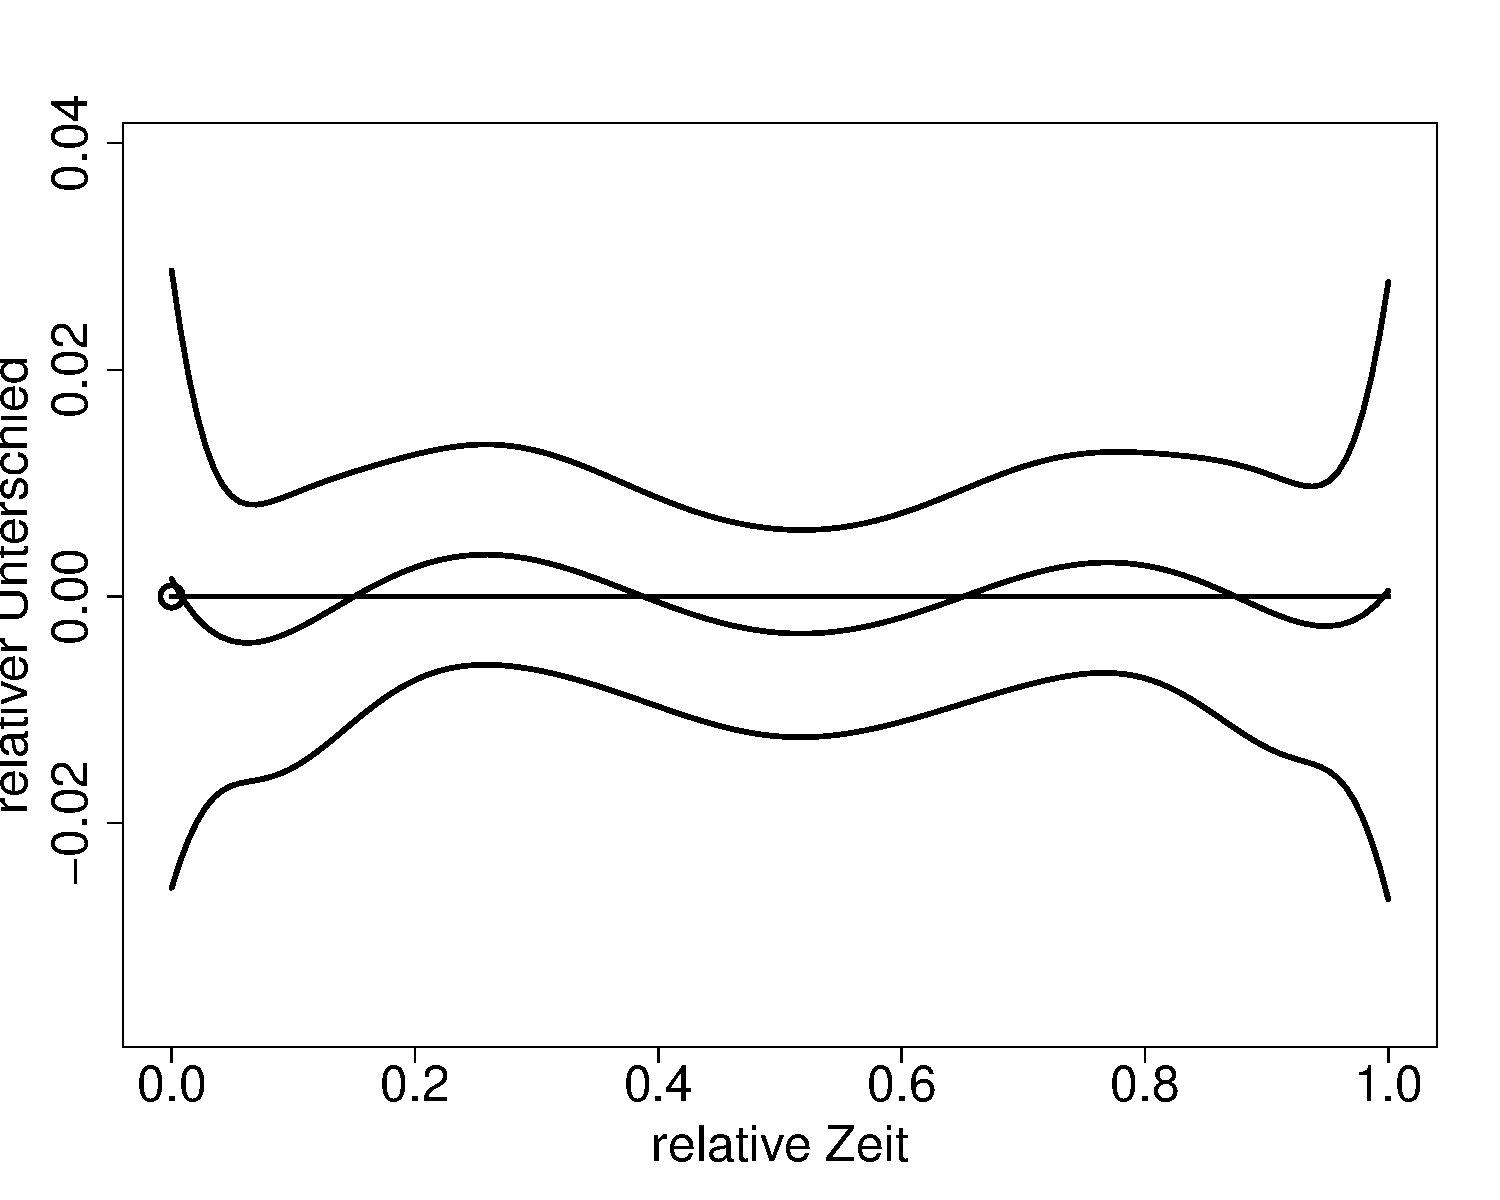
\includegraphics[width=0.5\textwidth]{30kPa-poly-KB-5-6.pdf}
  \caption{10 kPa Vergleich von Regressionsmodellen Grad Fünf versus Grad Sechs}
  \label{10kPa-Regmod-5-6}
\end{figure}

\begin{figure}[H] 
  \centering
     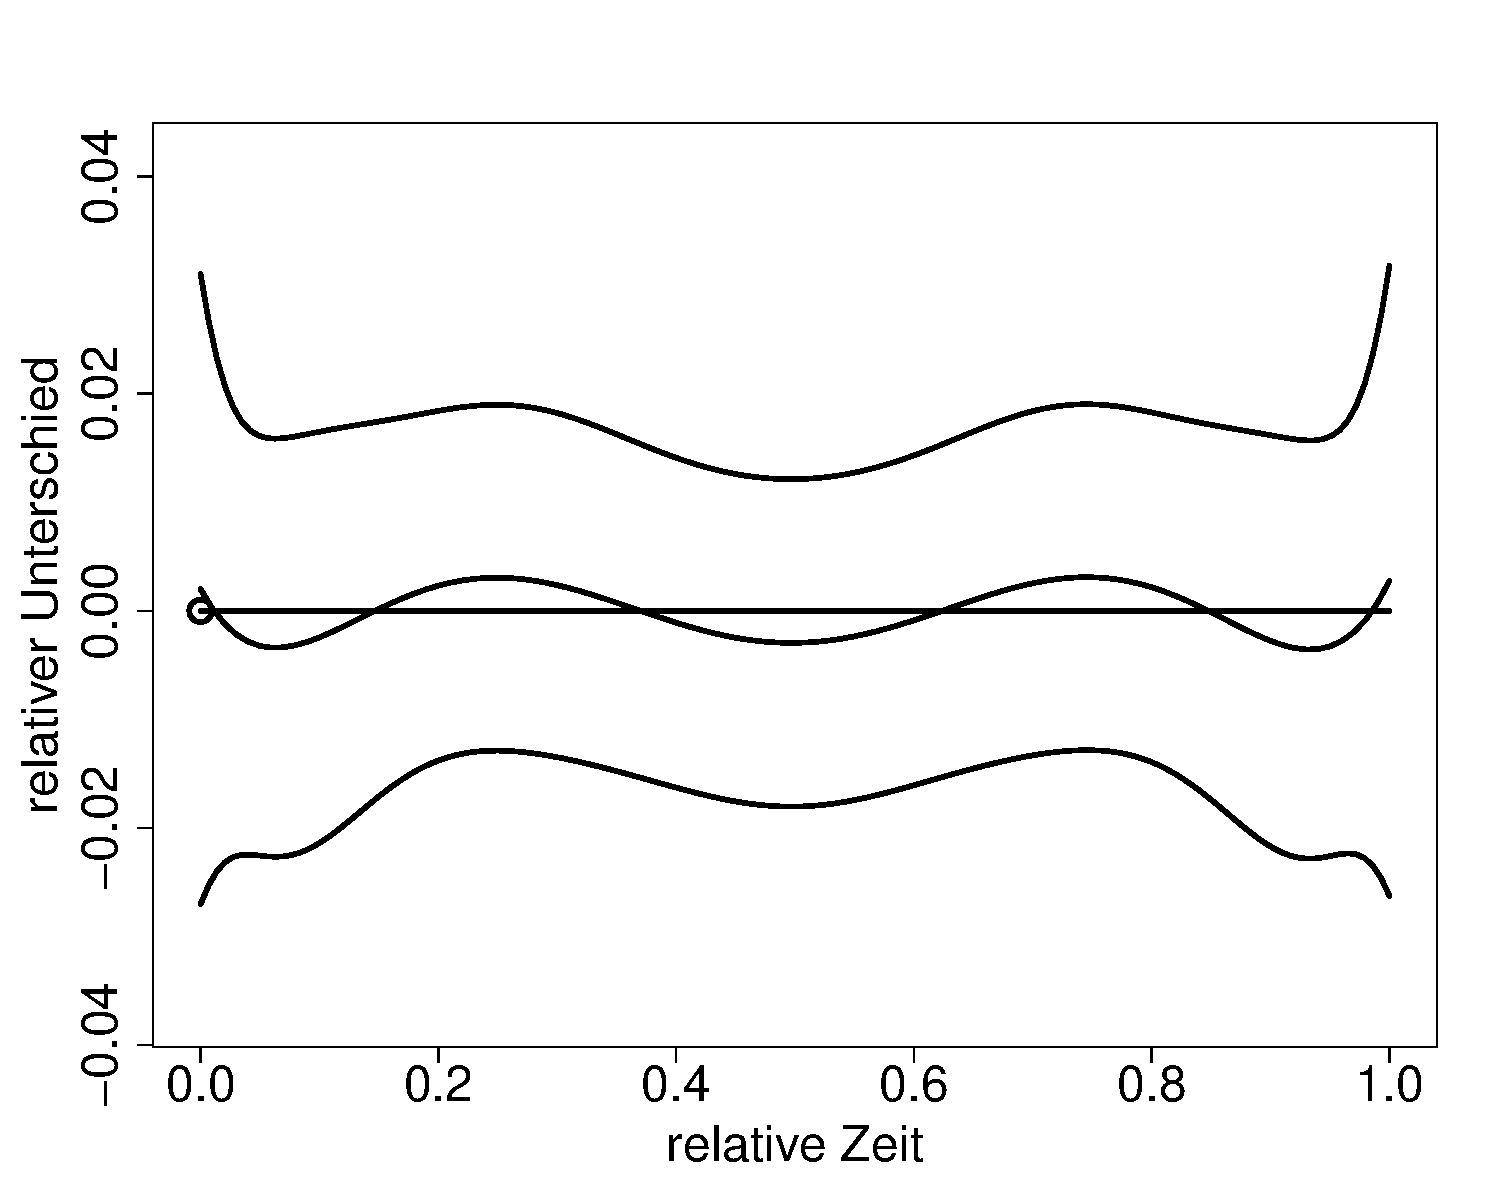
\includegraphics[width=0.5\textwidth]{10kPa-poly-KB-5-6.pdf}
  \caption{30 kPa Vergleich von Regressionsmodellen Grad Fünf versus Grad Sechs}
  \label{30kPa-Regmod-5-6}
\end{figure}

Man sieht, dass wieder in beiden Fällen die Nullhypothese nicht abgelehnt werden kann.


\subsection{Vergleich von 10 kPa und 30 kPa Daten}
Ziel dieses Abschnittes ist es die folgende Hypothese zu testen:

\begin{equation*}
H_0 : \beta_{10 kPa} = \beta_{30 kPa} \textbf{ vs. } H_1 : \beta_{10 kPa} \neq \beta_{30 kPa}
\end{equation*}

Dabei ist $\beta_{10 kPa}$ der Koeffizientenvektor einer Polynomregression vom Grad Fünf und $\beta_{30 kPa}$ der Koffizientenvektor einer Polynomregression vom gleichen Grad. 

Weiterhin gehen wir davon aus, dass dem Regressionsmodell vom Grad Fünf ein AR(1) Prozess zugrunde liegt. Außerdem verwenden wir die Methode aus Kapitel \ref{Vergleich von zwei Regressionsmodellen}, das heißt wir gehen davon aus, dass beide Prozesse das gleiche $\phi$ und $\sigma$ besitzen.

Zuerst plotten wir die beiden Datensätze mit den Regressionspolynomen in dieselbe Abbildung, um einen Überblick über ihre Ähnlichkeit zu bekommen. Dabei entsteht die Abbildung \ref{Vergleich-10-30}.


\begin{figure}[H] 
  \centering
     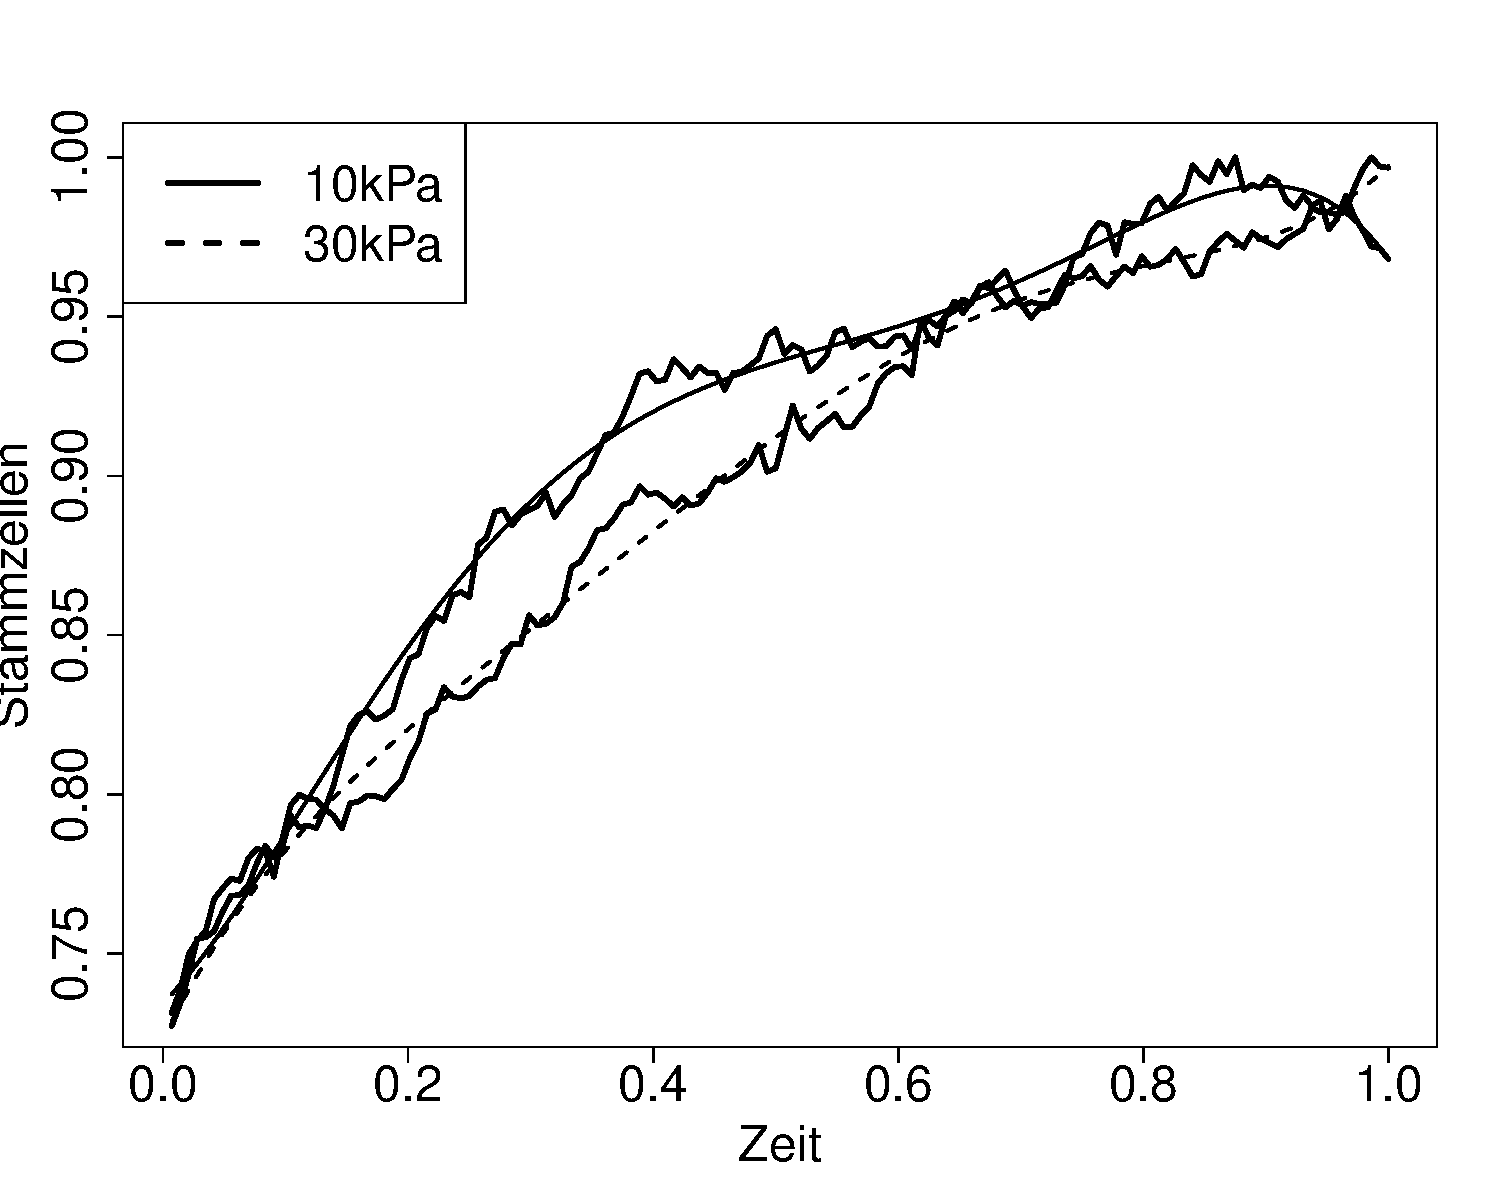
\includegraphics[width=0.65\textwidth]{Vergleich-10vs30-poly5}
  \caption{Vergleich von Regressionsmodellen}
  \label{Vergleich-10-30}
\end{figure}

Als Parameter bei der Regression erhält man für die 10 kPa Daten:

\begin{eqnarray*}
\hat{\beta} &=& (0.7343828 ;  0.3972789 ; 2.0659657 ; -8.1435038 ; 10.2153513 ; -4.3014467)  \\
\widehat{\sigma^2} &=& 0.007545373 \\
\hat{\phi} &=& 0.8225374
\end{eqnarray*}

und für die 30 kPa Daten:

\begin{eqnarray*}
\hat{\beta} &=& (0.7235374 ; 0.7708670 ; -2.3022522 ; 5.4896056 ; -6.1555617 ; 2.4709908) \\
\widehat{\sigma^2} &=& 0.009266164 \\
\hat{\phi} &=& 0.9039573
\end{eqnarray*}

Dies sind genau die selben Regressionsdaten aus Kapitel \ref{Vergleich verschiedener Konfidenzbänder}, allerdings diesmal mit einer anderen Fragestellung im Hintergrund.

Als nächstes wird die Differenz der Regressionsmodelle mit einem Konfidenzband in eine Abbildung geplottet. Dabei wird zur Erzeugung des kritischen Parameters die Methode für Konfidenzbänder auf einem Intervall, falls das Modell Polynomgestalt hat, angewendet.

\begin{figure}[H] 
  \centering
     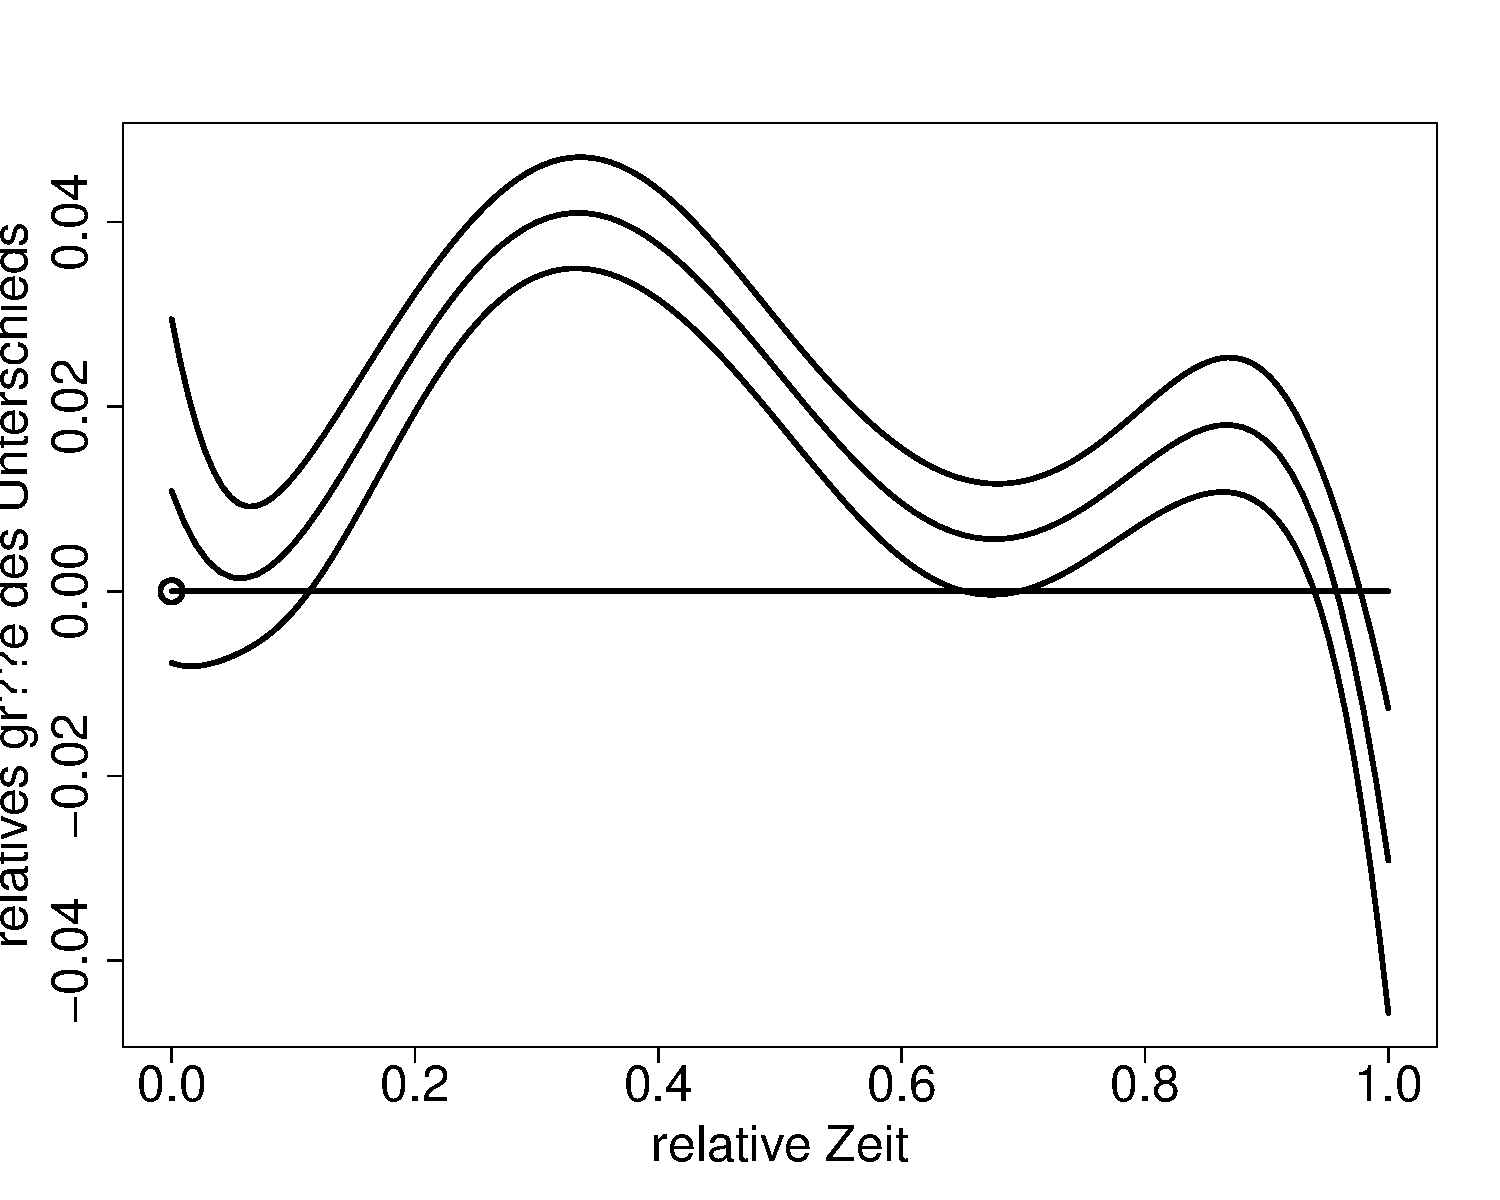
\includegraphics[width=0.5\textwidth]{Vergleich-10vs30kPa-poly5-KB}
  \caption{Vergleich von 10 kPa und 30 kPa Daten}
  \label{fig:10}
\end{figure}

Man sieht, dass die Nullfunktion nicht komplett im Konfidenzband enthalten ist. Man kann die Nullhypothese also verwerfen. Es gibt einen statistisch signifikanten Unterschied zwischen den beiden Regressionsmodellen.


\subsection{Einen Teil eines Regressionsmodells überprüfen}
Ziel dieses Abschnittes ist es, zu prüfen, ob bei den Stammzelldaten die ersten Koeffizienten des Koeffizientenvektors signifikant von Null verschieden sind.

Dazu führen wir für sowohl für die 10 kPa als auch für die 30 kPa Stammzelldaten je zwei Polynomregressionen durch. Wir legen dabei wieder eine Zeitreihe von der AR(1) Art zugrunde.

Dabei erhalten wir für die 10 kPa Daten die Werte:

\begin{eqnarray*}
\hat{\beta_{5}} &=&  (0.7373 ; 0.4219 ; 1.8730 ; -7.6992 ; 9.7893 ; -4.1542)  \\
\hat{\sigma_{5}^2} &=& 0.007545373 \\
\hat{\phi_{5}} &=& 0.8225374 \\
\hat{\beta_{6}} &=& (0.7352 ; 0.6265 ; -0.6151 ; 3.0831 ; -11.1962 ; 14.6223 ; -6.2906)  \\
\hat{\sigma_{6}^2} &=& 0.007205863 \\
\hat{\phi_{6}} &=& 0.8065796
\end{eqnarray*}

und für die 30 kPa Daten die Werte:

\begin{eqnarray*}
\hat{\beta_{5}} &=& (0.7288 ; 0.7345 ; -2.1594 ; 5.2097 ; -5.9029 ; 2.3864)  \\
\hat{\sigma_{5}^2} &=& 0.009266163 \\
\hat{\phi_{5}} &=& 0.9039573 \\
\hat{\beta_{6}} &=& (0.7273 ; 0.9495 ; -4.7664 ; 16.2343 ; -26.7566 ; 20.5211 ; -5.9124)  \\
\hat{\sigma_{6}^2} &=& 0.01673707 \\
\hat{\phi_{6}} &=& 0.9701881
\end{eqnarray*}

Um die Hypothese angeben zu können, definieren wir 

\begin{equation*}
\beta_{i} := (\beta_{i,1}, \beta_{i,2}, \ldots, \beta_{i,i}) \text{ für i=5,6 }
\end{equation*}

Damit können wir die folgenden Test durchführen.

\begin{eqnarray*}
&H_0 : \beta_{5,5} = 0 &\textbf{ vs. } H_1 : \beta_{5,5} \neq 0 \\
&H_0 : \beta_{6,6} = 0 &\textbf{ vs. } H_1 : \beta_{6,6} \neq 0 \\
&H_0 : (\beta_{6,5}, \beta_{6,6}) = (0,0) &\textbf{ vs. } H_1 : (\beta_{6,5}, \beta_{6,6}) \neq (0,0)
\end{eqnarray*}

Dazu verwendet man die Methode aus Abschnitt \ref{Teil eines Regressionsmodells überpruefen, wenn das Modell Polynomgestalt hat}. Wir verwerfen also die Nullhypothese, wenn die Konfidenzbänder $x_2' \cdot 0$ nicht vollkommen enthalten. 

Dabei ist in unserem Fall $x_2' \in \{0, 1/145, 2/145, \ldots, 144/145, 1 \}.$ 

In den Abbildungen \ref{10kPa Grad 5} und \ref{30kPa Grad 5} ist $x_2' \beta_{5,5}$ mit zugehörigem Konfidenzband eingezeichnet.

\begin{figure}[H] 
  \centering
     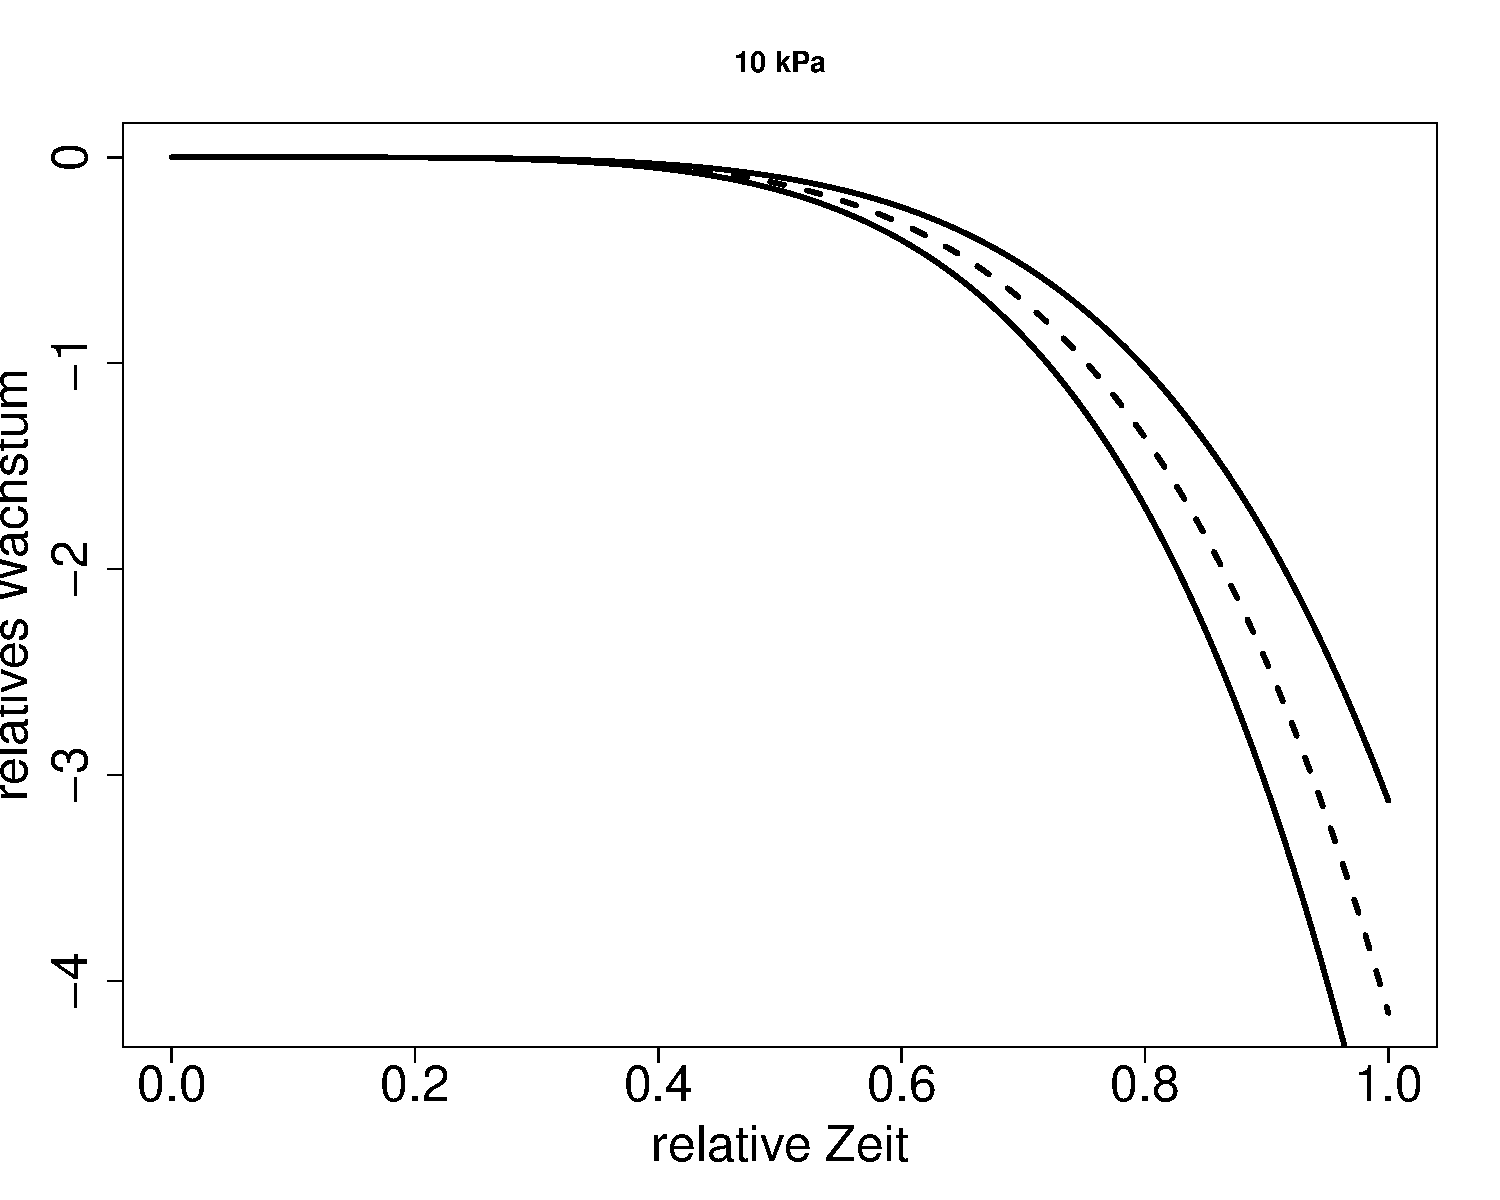
\includegraphics[width=0.5\textwidth]{10kPa-Grad-5-KB}
  \caption{10 kPa, Grad 5}
  \label{10kPa Grad 5}
\end{figure}

\begin{figure}[H] 
  \centering
     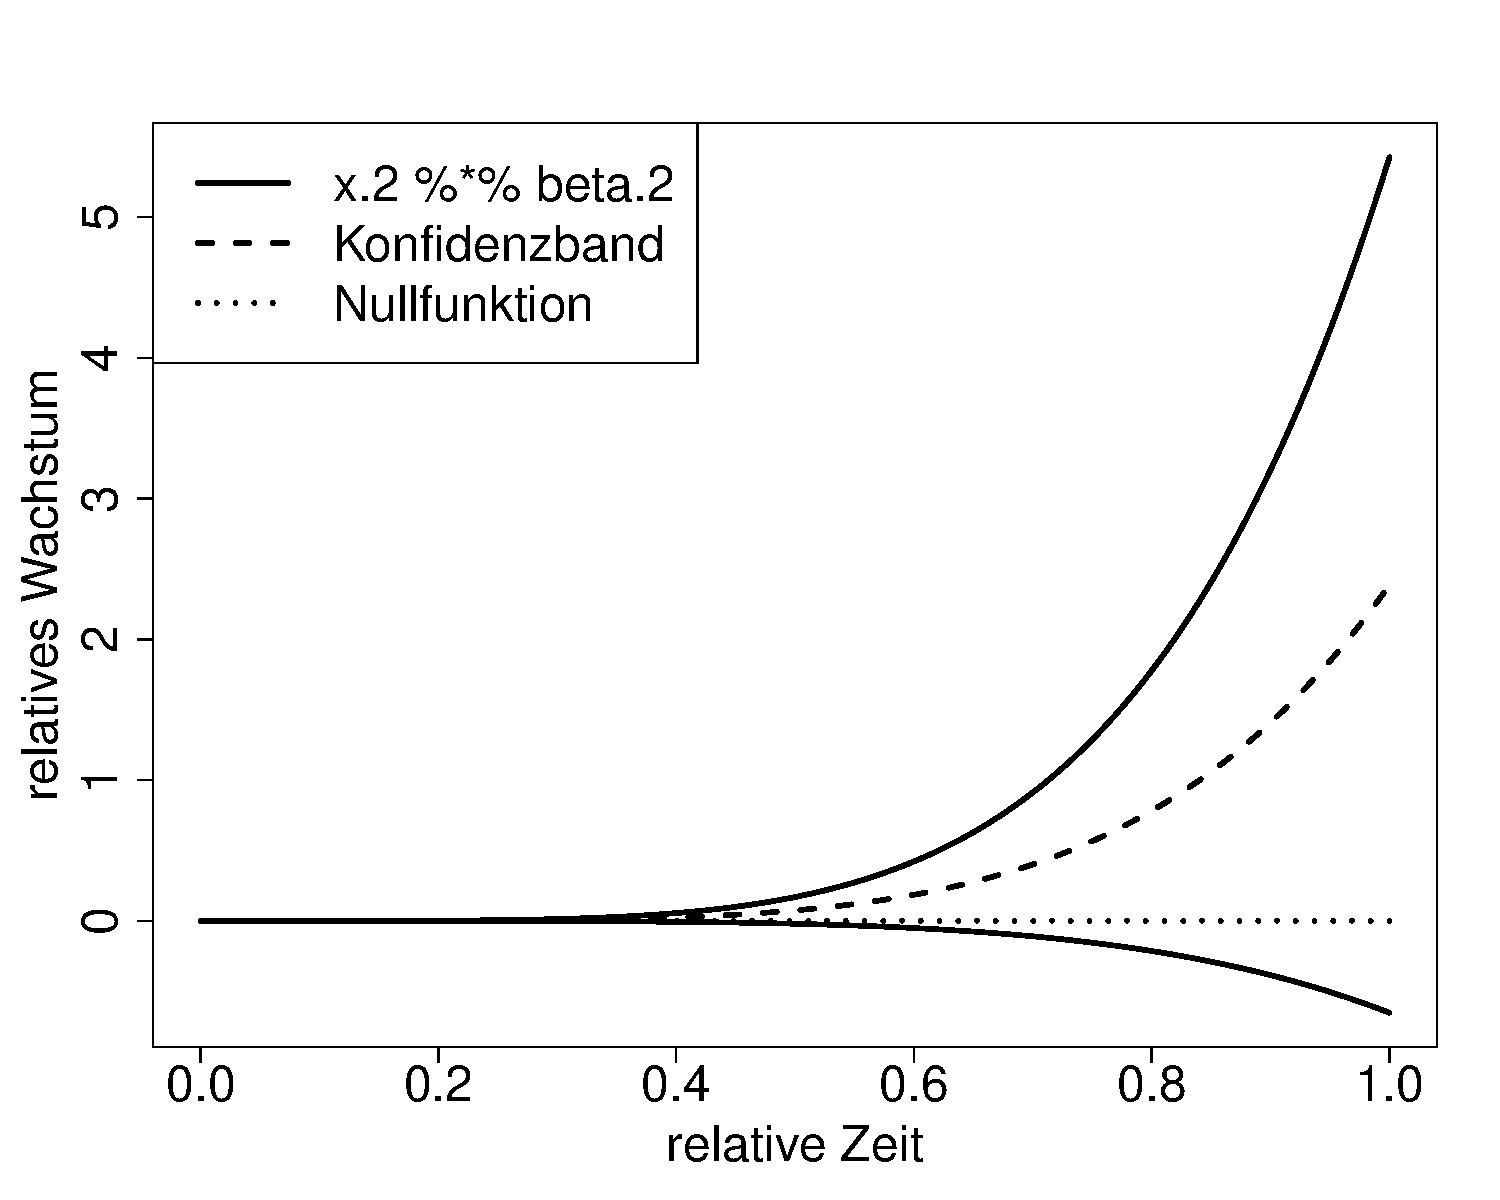
\includegraphics[width=0.5\textwidth]{30kPa-Grad-5-KB}
  \caption{30 kPa, Grad 5}
  \label{30kPa Grad 5}
\end{figure}

Man sieht deutlich, dass in beiden Fällen die Nullfunktion nicht vollständig im Konfidenzband enthalten ist. Wir können die Nullhypothese $H_0$ also verwerfen und haben einen Anhaltspunkt, davon auszugehen, dass $\beta_{5,5}$ in einem der beiden Fälle Null ist.

Die nächsten Abbildungen \ref{10kPa Grad 6.1} und \ref{30kPa Grad 6.1} geben  die Überprüfung von $\beta_{6,6}$ für die beiden Sätze an Stammzelldaten wieder.

\begin{figure}[H] 
  \centering
     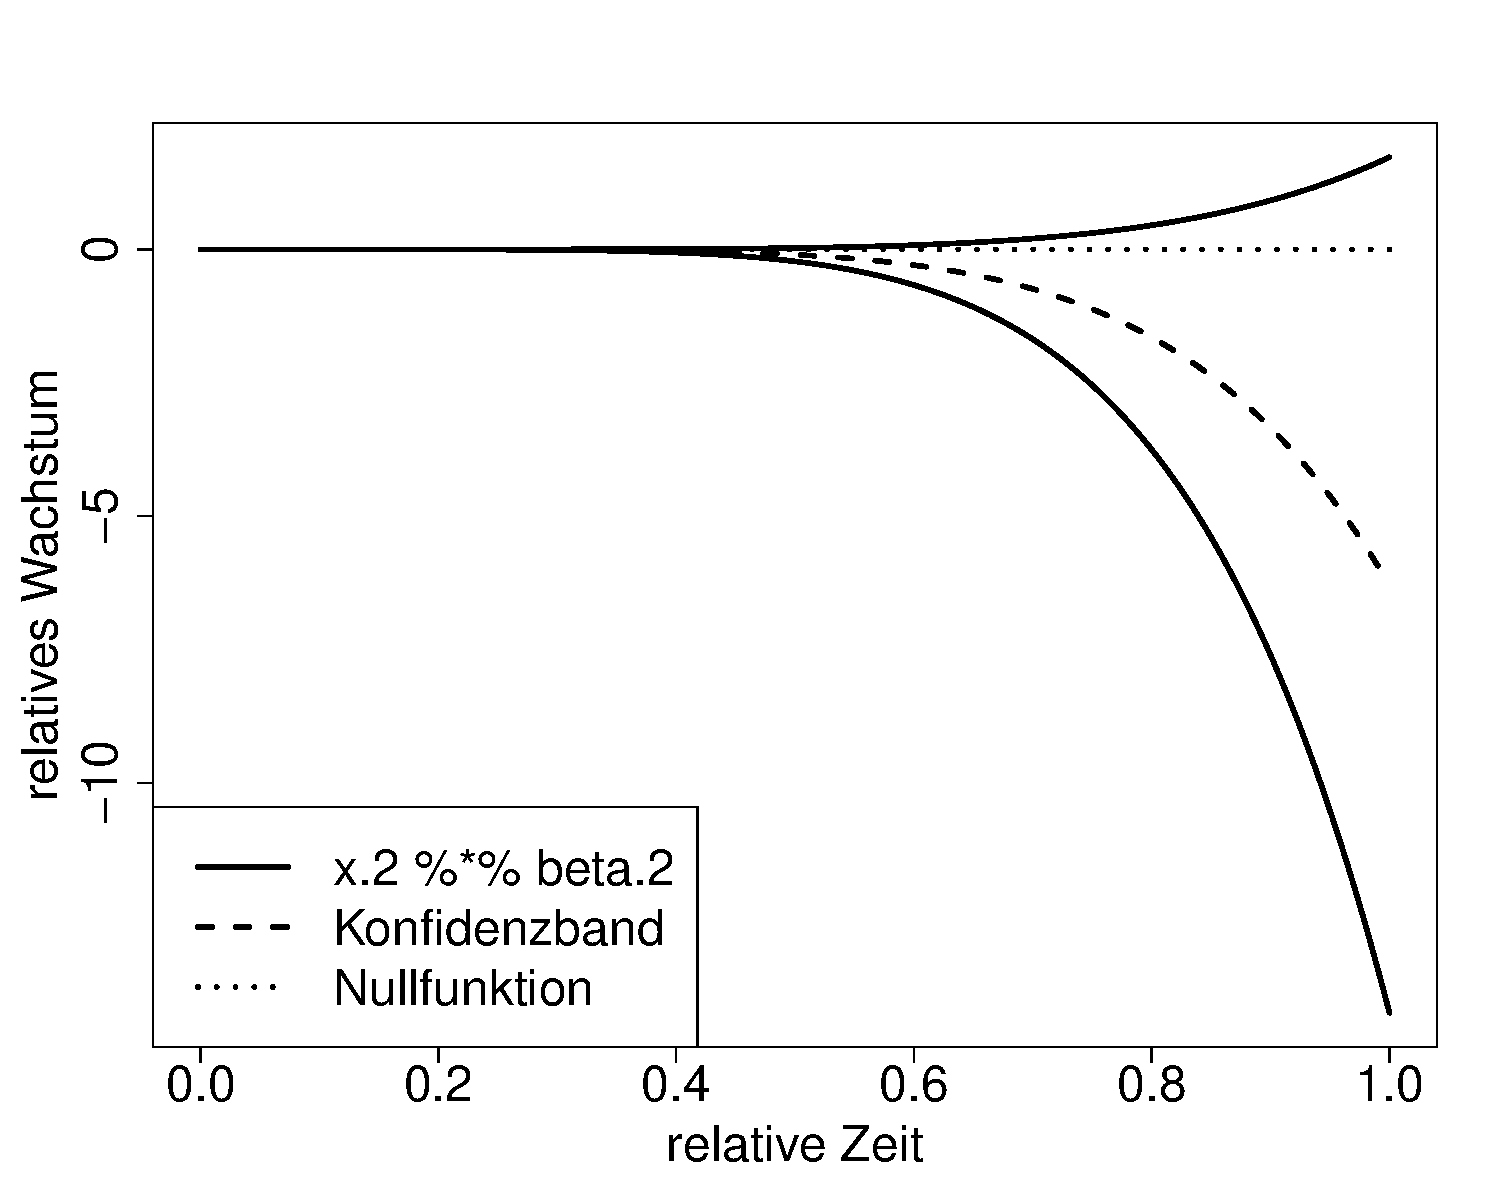
\includegraphics[width=0.5\textwidth]{10kPa-Grad-6-1-KB}
  \caption{10kPa, Grad 6, Test auf Grad Sechs}
  \label{10kPa Grad 6.1}
\end{figure}

\begin{figure}[H] 
  \centering
     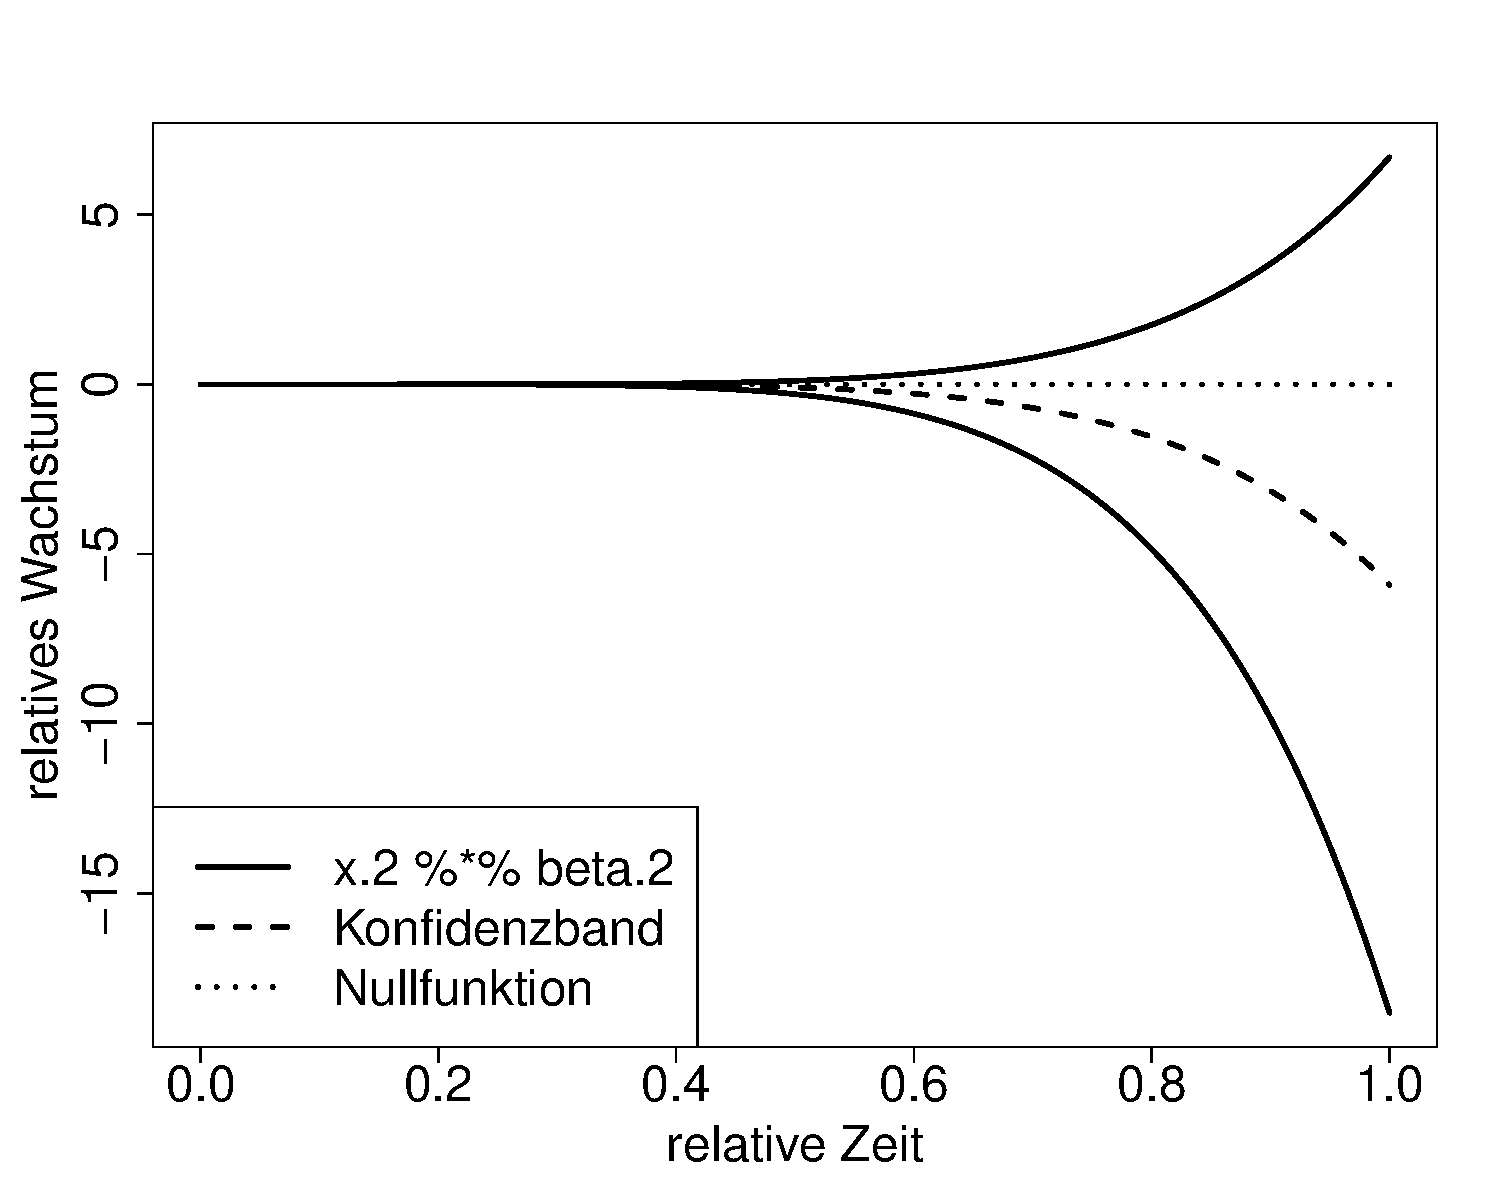
\includegraphics[width=0.5\textwidth]{30kPa-Grad-6-1-KB}
  \caption{30kPa Grad 6, Test auf Grad Sechs}
  \label{30kPa Grad 6.1}
\end{figure}

Man sieht, dass für die 10 kPa Daten die Nullfunktion wieder nicht ganz in dem Konfidenzband enthalten ist.

Bei den 30 kPa Daten ist dies jedoch der Fall. Damit kann die Nullhypothese abgelehnt werden und in diesem Fall gilt $\beta_{6,6} \neq 0$.

Betrachten wir zum Schluss den Test, ob $(\beta_{6,5}, \beta_{6,6}) = (0,0)$.

\begin{figure}[H] 
  \centering
     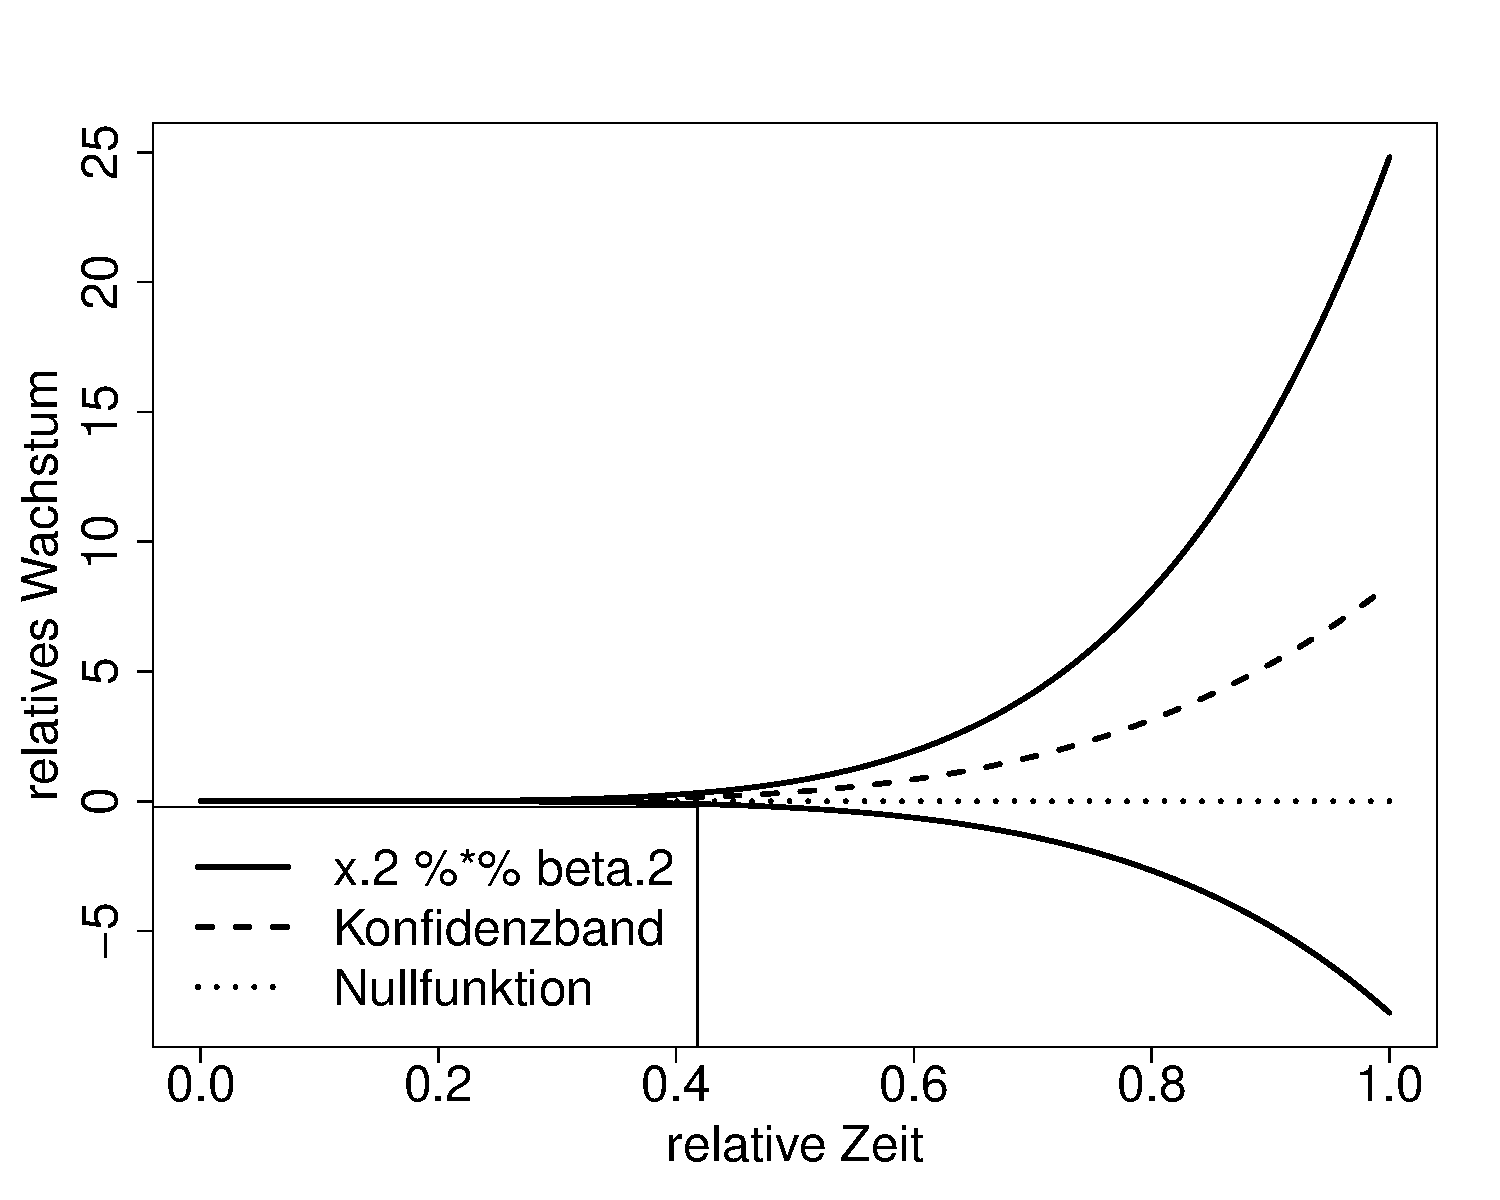
\includegraphics[width=0.5\textwidth]{10kPa-Grad-6-2-KB}
  \caption{10 kPa, Grad 6, Test auf Grad Fünf}
  \label{10kPa Grad 6.2}
\end{figure}

\begin{figure}[H] 
  \centering
     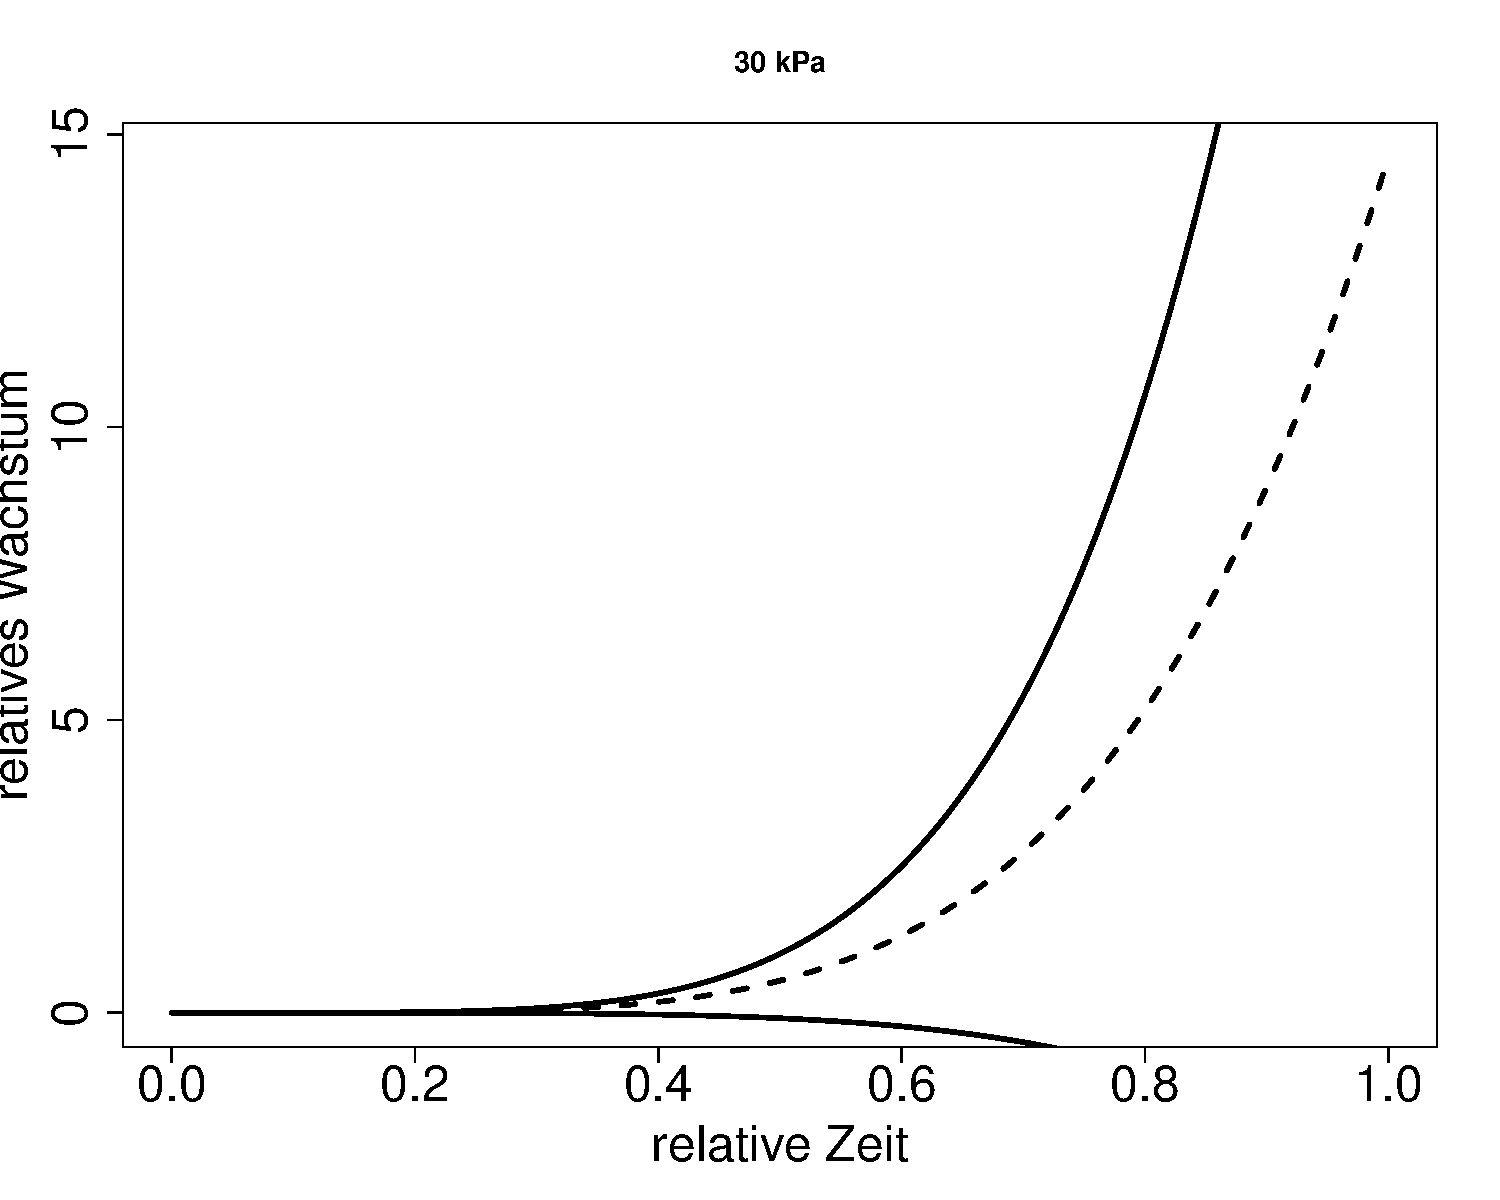
\includegraphics[width=0.5\textwidth]{30kPa-Grad-6-2-KB}
  \caption{30 kPa, Grad 6, , Test auf Grad Fünf}
  \label{30kPa Grad 6.2}
\end{figure}

Auch hier sieht man, dass für die 10 kPa Daten die Nullfunktion wieder nicht ganz in dem Konfidenzband enthalten ist. Deshalb kann auch in diesem Fall $H_0$ nicht verworfen werden.

Bei den 30 kPa Daten ist dies jedoch der Fall. Damit kann die Nullhypothese abgelehnt werden und in diesem Fall gilt $\beta_{6,6} \neq 0$.



\newpage
\section*{Fazit}
In dieser Bachelorarbeit haben wir Methoden behandelt, um Regressionsmodelle zu vergleichen. Dazu wurde eine Verbesserung des normalerweise verwendeten F-Tests mittles auf Konfidenzbändern basierender Methoden nach \cite{Liu64} betrachtet.

Dabei wurden die Methoden in \cite{Liu64} auf den Fall von abhängigen Daten mit einer Abhängigkeitsstruktur der Art AR(1) verallgemeinert.

Insbesondere für Regressionsmodelle mit Polynomgestalt auf einem Polyeder waren die durchgeführten Tests aussagekräftig, die diese speziellen Anforderungen an den Test berücksichtigt haben. Dies sieht man daran, dass sich kleinere kritische Konstanten für die Konfidenzbänder ergeben haben. 

Allerdings ist die Rechenzeit gerade für diese Methode sehr lang, da eine Monte-Carlo Simulation durchgeführt werden muss. Diese lange Rechenzeit hat sich auch negativ auf die Ergebnisse der simulationsweisen Bestimmung der Überdeckungswahrscheinlichkeiten ausgewirkt.

Die Methode Konfidenzbänder auf ganz $\mathbb{R}^p$ zu bestimmen war schneller und lieferte zum Teil bessere Überdeckungswahrscheinlichkeiten.

Die in dieser Ausarbeitung verwendeten R und C++ Codes sind in dem Paket KBminmaxpoly auf der Seite 

\begin{center}
\textit{https://github.com/fake1884/KBminmaxpoly} 
\end{center}

gefunden werden.





\nocite{Hsu41}

\newpage
\printbibliography


\newpage
\section*{Selbstständigkeitserklärung}
\addcontentsline{toc}{section}{Selbstständigkeitserklärung}
Hiermit bestätige ich, dass ich die vorliegende Arbeit selbstständig, nur mit Hilfe meiner Betreuer und ohne Benutzung anderer als der angegebenen Hilfsmittel angefertigt habe. Die aus fremden Quellen (einschließlich elektronischer Quellen) direkt oder indirekt übernommenen Gedanken sind ausnahmslos als solche kenntlich gemacht. Die Arbeit ist in gleicher oder ähnlicher Form oder auszugsweise im Rahmen einer anderen Prüfung noch nicht vorgelegt worden.
\\ \\ \\ \\
\parbox{5cm}{\centering Göttingen, }
%\hrule \strut \centering\footnotesize Ort, Datum} 
\hfill\parbox{4cm}{\hrule \strut \centering  \footnotesize Henning Hause}
\end{document}